% =====================================================================
%  BÁO CÁO ĐỒ ÁN TỐT NGHIỆP — Hệ thống quản lý bãi giữ xe thông minh
%  Trường Đại học Công nghệ Thông tin (UIT) — ĐHQG-HCM
%  Engine: XeLaTeX   |   Build: latexmk -xelatex main.tex  (xem PLAN.md)
%  Cấu trúc: main.tex -> preamble.tex + frontmatter/ + chapters/ + appendices/
% =====================================================================
\documentclass[13pt,a4paper,oneside]{report}

% ---------- Thông tin đề tài (chỉnh ở đây, dùng lại toàn báo cáo) ----------
\newcommand{\ThesisTitleVi}{Nghiên cứu và xây dựng hệ thống quản lý bãi giữ xe thông minh ứng dụng thị giác máy tính và Edge AI}
\newcommand{\ThesisTitleEn}{Research and Development of a Smart Parking Management System Using Computer Vision and Edge AI}
\newcommand{\ThesisTitleShort}{Hệ Thống Bãi Giữ Xe Thông Minh}   % dùng cho header
\newcommand{\Supervisor}{ThS. Phan Đình Duy}
\newcommand{\StudentA}{Nguyễn Minh Nhật}
\newcommand{\StudentAId}{25410104}
\newcommand{\StudentB}{Lê Quang Hoài Đức}
\newcommand{\StudentBId}{25410034}
\newcommand{\AcademicYear}{2025 -- 2026}
\newcommand{\DefenseDate}{Thành phố Hồ Chí Minh, tháng 9 năm 2026}

% =====================================================================
%  preamble.tex — gói, font, header/footer, định dạng tiêu đề
%  Bám định dạng file mẫu (Nhom_6-CS340...): Times, header 2 bên,
%  Chương N. / N.M. / N.M.K., hình/bảng đánh số toàn cục, IEEE refs.
% =====================================================================

% ---------- Ngôn ngữ & font (XeLaTeX) ----------
\usepackage{fontspec}
\usepackage[vietnamese]{babel}     % tự dịch: Hình, Bảng, Chương, Mục lục, Danh sách hình vẽ...
% Font chính: Times New Roman (có sẵn trên macOS/Windows, đủ glyph tiếng Việt).
% Linux: cài msttcorefonts hoặc đổi sang "Liberation Serif" / "TeX Gyre Termes".
\setmainfont{Times New Roman}
\setmonofont{Menlo}[Scale=0.85]   % đường dẫn, tên file, tên biến
% \setmainfont{TeX Gyre Termes}    % <- fallback đa nền tảng (cần gói tex-gyre)

% ---------- Trình bày trang ----------
\usepackage[a4paper,left=3cm,right=2cm,top=2.5cm,bottom=2.5cm]{geometry}
\usepackage{setspace}
\onehalfspacing
\usepackage{indentfirst}           % thụt lề dòng đầu mỗi đoạn (chuẩn VN)
\setlength{\parindent}{1cm}

% ---------- TikZ (UML diagrams: ER, sequence, use case, class — Ch7) ----------
\usepackage{tikz}
\usetikzlibrary{positioning,shapes.geometric,arrows.meta,fit,calc}

% ---------- Đồ họa, bảng, màu ----------
\usepackage{graphicx}
\graphicspath{{figures/}}
% Quy ước ảnh: MỌI \includegraphics viết KHÔNG ĐUÔI, ví dụ
%   
\includegraphics[width=0.8\textwidth]{eda_class_distribution}
% XeLaTeX bắt .pdf (vector, nét khi in), pandoc bắt .png (nhúng được vào .docx).
% Thứ tự ưu tiên dưới đây quyết định điều đó cho phía XeLaTeX.
\DeclareGraphicsExtensions{.pdf,.png,.jpg}
\usepackage{booktabs}
\usepackage{multirow}
\usepackage{array}
\usepackage{longtable}
\usepackage{xcolor}
\definecolor{uitblue}{RGB}{0,84,159}
\usepackage[font=small,labelfont=bf]{caption}
\usepackage{enumitem}
\usepackage{amsmath,amssymb}
\usepackage{siunitx}               % số & đơn vị, dấu phẩy thập phân theo quy ước VN
\sisetup{output-decimal-marker={,}, group-separator={.}, group-minimum-digits=4}

% ---------- Hình/bảng đánh số THEO CHƯƠNG (Hình 3.1, Bảng 3.1) như BieuMau ----------
\counterwithin{figure}{chapter}
\counterwithin{table}{chapter}
\renewcommand{\thefigure}{\thechapter.\arabic{figure}}
\renewcommand{\thetable}{\thechapter.\arabic{table}}

% ---------- Header / footer 2 bên (fancyhdr) ----------
\usepackage{fancyhdr}
\pagestyle{fancy}
\fancyhf{}
\fancyhead[L]{\small UIT -- Đồ án tốt nghiệp}
\fancyhead[R]{\small \ThesisTitleShort{} -- \StudentA{} \& \StudentB}
\fancyfoot[C]{\thepage}
\renewcommand{\headrulewidth}{0.4pt}
\renewcommand{\footrulewidth}{0pt}
% Trang mở đầu chương cũng giữ header giống file mẫu:
\fancypagestyle{plain}{%
  \fancyhf{}%
  \fancyhead[L]{\small UIT -- Đồ án tốt nghiệp}%
  \fancyhead[R]{\small \ThesisTitleShort{} -- \StudentA{} \& \StudentB}%
  \fancyfoot[C]{\thepage}%
  \renewcommand{\headrulewidth}{0.4pt}%
}

% ---------- Định dạng tiêu đề: chương ngắt trang, tên IN HOA ----------
\usepackage{titlesec}
\titleformat{\chapter}[hang]
  {\normalfont\fontsize{14}{17}\bfseries}
  {\chaptertitlename\ \thechapter.}{0.6em}{\MakeUppercase}
\titlespacing*{\chapter}{0pt}{0pt}{20pt}
\titlelabel{\thetitle.\quad}       % dấu chấm sau số mục: "1.1.", "1.1.1."

% ---------- Thư mục tài liệu tham khảo IEEE ----------
\usepackage[backend=biber,style=ieee,sorting=nyt]{biblatex}
\DeclareSourcemap{\maps[datatype=bibtex]{\map{\step[fieldsource=langid, final]\step[fieldset=keywords, origfieldval]}}}
\addbibresource{refs.bib}

% ---------- Liên kết ----------
\usepackage[hidelinks]{hyperref}

% ---------- Tiện ích soạn thảo: đánh dấu phần CHƯA VIẾT ----------
% Dùng \wip{ghi chú} để chèn ghi chú "đang làm" nổi bật (dễ tìm khi rà soát).
\newcommand{\wip}[1]{\textcolor{red}{\textbf{[TODO: #1]}}}
% Dùng \ph{...} cho số liệu placeholder cần thay bằng kết quả thật.
\newcommand{\ph}[1]{\textcolor{orange}{\underline{#1}}}


\begin{document}

% ============================ FRONT MATTER ============================
% ---------- Trang bìa (bám mẫu file Nhom_6) ----------
\begin{titlepage}
\thispagestyle{empty}
\centering

{\large ĐẠI HỌC QUỐC GIA THÀNH PHỐ HỒ CHÍ MINH\par}
{\large TRƯỜNG ĐẠI HỌC CÔNG NGHỆ THÔNG TIN\par}

\vspace{0.6cm}
% Logo (tùy chọn): đặt file figures/logo-uit.png rồi bỏ chú thích dòng dưới.
% \includegraphics[width=3cm]{logo-uit.png}\par

\vspace{1.8cm}
{\Large\bfseries\MakeUppercase{\ThesisTitleVi}\par}

\vspace{0.5cm}
{\itshape \ThesisTitleEn\par}

\vspace{1.6cm}
{\large Báo cáo đồ án tốt nghiệp\par}
{\large Ngành: [Kỹ thuật Máy tính / ... — điền ngành]\par}

\vspace{1.4cm}
\begin{flushleft}\hspace{2.5cm}
\begin{tabular}{@{}ll@{}}
\textbf{Giảng viên hướng dẫn:} & \Supervisor \\[4pt]
\textbf{Nhóm thực hiện:} & \\
 & \StudentA{} -- \StudentAId \\
 & \StudentB{} -- \StudentBId \\[4pt]
\textbf{Niên học:} & \AcademicYear \\
\end{tabular}
\end{flushleft}

\vfill
{\large \DefenseDate\par}

\end{titlepage}


\pagenumbering{roman}
\setcounter{page}{1}

% ---------- Tóm tắt nội dung (bám mẫu: heading canh giữa + Từ khóa) ----------
\chapter*{Tóm tắt nội dung}
\addcontentsline{toc}{chapter}{Tóm tắt nội dung}

Đề tài
xây dựng hệ thống quản lý bãi giữ xe thông minh nhận diện phương tiện bằng thị giác máy
tính, thiết kế độc lập nền tảng và ưu tiên thiết bị biên (Edge AI) nhằm giảm phụ thuộc
máy chủ và bảo vệ dữ liệu cá nhân theo Luật Bảo vệ dữ liệu cá nhân.

Hệ thống thực hiện năm bước suy luận trên cùng khung ảnh: phát hiện xe, phân loại loại
xe và kiểu dáng, phát hiện biển số, nhận màu nền biển và đọc ký tự (OCR), với bảng ký
tự OCR mở rộng 37 ký tự. Nghiệp vụ gồm cơ sở dữ liệu, logic vào
ra, đối chiếu chống gian lận, tính phí và dashboard; toàn bộ pipeline xuất ONNX để dùng
chung một bộ mã trên máy tính lẫn Raspberry Pi 5.

Phát hiện biển đạt mAP@0,5 bằng 0,983 sau khử trùng lặp gần; OCR đọc đúng cả biển
91,9\% trên tập ảnh camera cổng, 80,2\% và 56,6\% trên hai tập độc lập; phân loại loại
xe 98,66\% (ResNet18) và kiểu dáng 90,07\% (MobileNetV3-Small). Trên Raspberry Pi 5, độ
trễ đầu cuối trung vị 0,464 giây mỗi lượt xe, dưới ngưỡng hai giây, kết quả khớp tuyệt
đối máy tính trên toàn bộ ảnh cổng thử nghiệm.
       % Tóm tắt nội dung + Từ khóa

\tableofcontents
\listoffigures
\listoftables

% ============================ MAIN MATTER ============================
\cleardoublepage
\pagenumbering{arabic}
\setcounter{page}{1}

% =====================================================================
%  CHƯƠNG 1. GIỚI THIỆU                           | Phụ trách: Cả 2
%  Ngân sách: mục tiêu 5 trang, trần 6,0 trang
%  Nguồn: docs/DCDATN_25410104_NguyenMinhNhat_25410034_LeQuangHoaiDuc.pdf,
%         README.md, src/ml/pipeline/onnx_pipeline.py (mô tả pipeline)
% =====================================================================
\chapter{Giới Thiệu}
\label{ch:gioithieu}

\section{Bối Cảnh và Động Lực}

Nhu cầu quản lý bãi giữ xe tại Việt Nam tăng nhanh theo mật độ phương tiện cá nhân.
Phần lớn bãi xe vẫn vận hành thủ công hoặc bằng thẻ từ: nhân viên kiểm tra thẻ hoặc biển số bằng mắt, ghi chép giấy và thu
phí trực tiếp. Cách làm này tốn nhân lực ở cổng, dễ sai sót khi đối chiếu xe vào ra,
không lưu bằng chứng hình ảnh khi tranh chấp và không tạo ra dữ liệu vận hành để thống
kê lưu lượng, doanh thu hay phát hiện bất thường.

Thị giác máy tính và các mô hình phát hiện đối tượng hiện đại cho phép tự động hóa
khâu nhận diện tại cổng, thay quy trình thẻ từ bằng luồng chụp ảnh, phân tích và ghi
nhận tức thì. Mỗi lượt xe trở thành một bản ghi có thời gian, biển số, loại xe và ảnh
toàn cảnh, mở ra khả năng thống kê và phân tích lưu thông.

Xu hướng đưa suy luận xuống thiết bị biên ngày càng rõ trong các hệ thống bãi xe thông
minh~\autocite{pradhan2025iotparking,arukonda2026smartparking,rani2024ips}. Truyền video
từ camera cổng lên máy chủ hoặc cloud có ba nhược điểm: độ trễ tăng khi đường truyền
nghẽn, chi phí máy chủ và băng thông tăng theo số lượng bãi xe, và ảnh phương tiện cùng
biển số liên tục ra ngoài mạng nội bộ. Nhược điểm cuối đáng lưu ý khi Luật Bảo vệ dữ liệu
cá nhân (hiệu lực 01/01/2026) xếp biển số và ảnh nhận dạng vào dữ liệu cá nhân cần kiểm
soát truy cập và hạn chế lưu trữ~\autocite{vn2025lutbvdlcn}. Suy luận tại biên xử lý ngay
tại chỗ, chỉ ghi thông tin thiết yếu vào cơ sở dữ liệu, không truyền video thô ra ngoài.

Các kỹ thuật tối ưu như lượng tử hóa (quantization) và chuyển sang định dạng ONNX đã
thu hẹp khoảng cách hiệu năng giữa thiết bị biên và máy
chủ~\autocite{mdpi2026sbcbenchmark,sonnara2025lightedge}. Raspberry Pi 5 với CPU ARM
Cortex-A76 đủ sức chạy các mô hình phát hiện cỡ nano ở tốc độ chấp nhận được sau khi
xuất ONNX. Đề tài đặt trọng tâm vào việc chạy trọn vẹn một hệ thống quản lý bãi xe
trên một thiết bị biên đơn lẻ, thay vì chỉ dừng ở khâu nhận dạng.

\section{Vấn Đề Đặt Ra}

\textbf{Đặc thù biển số Việt Nam.}
Ô tô dùng biển một hàng, xe máy dùng biển hai hàng, đòi hỏi bước tách dòng trước khi
đọc ký tự; biển hai hàng gần như không xuất hiện trong dữ liệu quốc tế nên các pipeline
ALPR thông dụng xử lý sai hoặc bỏ sót. Seri MĐ và TĐ của xe máy điện lại chứa ký tự
``Đ'' nằm ngoài bảng ký tự của các engine OCR tiếng
Anh~\autocite{tran2025vietnamlpr,le2023motorcycleplate}, nên không thể tái sử dụng trực
tiếp mô hình huấn luyện cho biển số nước ngoài.

\textbf{Thiếu dữ liệu phù hợp.}
Chưa có bộ dữ liệu bãi xe Việt Nam nào gán nhãn đồng thời cho biển số, loại xe và màu
nền biển; các bộ quốc tế như CCPD hay UFPR-ALPR chỉ có vùng biển và ký tự. Phần lớn ảnh
công khai trong nước chụp ở điều kiện ánh sáng tốt, không đại diện cho cổng bãi xe thực
tế với ngược sáng, mưa hay đêm tối. Ghép nhiều nguồn không đồng nhất đòi hỏi làm sạch,
chuẩn hóa nhãn và kiểm soát rò rỉ giữa tập huấn luyện và kiểm tra.

\textbf{Ràng buộc tài nguyên thiết bị biên.}
Thiết bị biên có RAM hạn chế và không có GPU rời, buộc mô hình phải nhỏ và được tối ưu
mới đạt độ trễ chấp nhận được~\autocite{mdpi2026sbcbenchmark,sonnara2025lightedge}.
Pipeline gọi năm bước suy luận liên tiếp trên cùng một khung ảnh nên độ trễ tích lũy
theo chiều dài pipeline; đạt mục tiêu dưới hai giây trên Raspberry Pi 5 đòi hỏi chọn cẩn
thận kích thước mô hình, độ phân giải đầu vào và định dạng tối ưu cho từng bước.

\textbf{Thiếu hệ thống end-to-end có nghiệp vụ.}
Phần lớn công trình dừng ở nhận dạng biển số, không xử lý phiên gửi xe, đối chiếu chống
gian lận và tính phí, nên khoảng cách tới một sản phẩm vận hành được vẫn còn lớn. Một
bãi xe thật cần phân biệt xe vào và xe ra trên cùng biển số, phát hiện biển số vào không
khớp biển số ra (xe hoán đổi biển), áp biểu phí theo nhóm phương tiện, lưu ảnh toàn cảnh
làm bằng chứng và có giao diện tra cứu thời gian thực.

\section{Câu Hỏi Nghiên Cứu}
\label{sec:cauhoi}

Từ các vấn đề trên, câu hỏi nghiên cứu trung tâm được phát biểu như sau: \emph{làm thế
nào để xây dựng một hệ thống quản lý bãi giữ xe tự động hóa khâu nhận diện phương tiện
Việt Nam, vận hành hoàn chỉnh trên thiết bị biên giá rẻ chỉ dùng CPU, đạt độ chính xác
và tốc độ đáp ứng yêu cầu thực tế, đồng thời tuân thủ quy định bảo vệ dữ liệu cá nhân?}
Câu hỏi này được cụ thể hóa thành bốn câu hỏi thành phần:

\begin{enumerate}[leftmargin=*, label=\textbf{CH\arabic*.}]
  \item \textbf{Độ tin cậy.} Hệ thống xác định thông tin phương tiện (biển số, loại xe) từ ảnh cổng chính xác đến đâu, và các thuật toán nghiệp vụ (đối chiếu phiên, tính phí) xử lý thế nào khi mô hình nhận dạng sai?
  \item \textbf{Tối ưu tài nguyên.} Trên phần cứng chỉ có CPU, cần cân bằng độ chính xác, độ trễ và điện năng ra sao để mỗi lượt xe xử lý dưới hai giây?
  \item \textbf{Phương pháp dữ liệu.} Khi chưa thu được dữ liệu thực địa, việc kết hợp các bộ dữ liệu công khai có đủ đại diện để huấn luyện và đánh giá không, và cần kiểm soát gì để tránh đánh giá thiên lệch?
  \item \textbf{Bảo mật và riêng tư.} Cơ chế lưu trữ và tra cứu biển số, ảnh phương tiện cần thiết kế thế nào để không rò rỉ dữ liệu cá nhân, đáp ứng Luật Bảo vệ dữ liệu cá nhân?
\end{enumerate}

\section{Mục Tiêu, Phạm Vi và Tiêu Chí Thành Công}

\subsection{Mục Tiêu Tổng Quát}

Mục tiêu tổng quát là xây dựng một hệ thống quản lý bãi giữ xe thông minh, tự động nhận
diện biển số, loại xe và màu nền biển, thiết kế độc lập nền tảng và ưu tiên triển khai
trên thiết bị biên. Hệ thống gồm cả phần suy luận thị giác máy tính lẫn nghiệp vụ quản
lý vào ra, tính phí và dashboard thống kê, chạy được trên máy chủ, PC và thiết bị biên
với cùng một bộ mã nguồn.

\subsection{Mục Tiêu Cụ Thể}

Năm mục tiêu cụ thể theo đề cương:

\textbf{Mục tiêu 1: Mô đun nhận diện biển số.}
Phát hiện vùng biển số và đọc ký tự (OCR) cho cả biển một hàng của ô tô và biển hai
hàng của xe máy, xử lý đúng ký tự ``Đ'' trong seri biển xe máy điện.

\textbf{Mục tiêu 2: Phân loại phương tiện và nhận màu nền biển.}
Phân loại phương tiện theo bốn lớp (ô tô, xe máy, xe tải, xe buýt) và nhận màu nền biển
(trắng, vàng, xanh, đỏ) để phân nhóm xe cá nhân, kinh doanh và cơ quan nhà nước theo
quy định về biển số của Bộ Công an.

\textbf{Mục tiêu 3: Cơ sở dữ liệu và logic quản lý vào ra.}
Ghi nhận thời gian vào ra, đối chiếu biển số để phát hiện gian lận, lưu ảnh toàn cảnh
làm bằng chứng và tính phí tự động theo nhóm phương tiện.

\textbf{Mục tiêu 4: Dashboard quản lý và thống kê.}
Theo dõi xe ra vào theo thời gian thực, tra cứu phương tiện trong bãi, thống kê theo
loại xe, màu biển, lưu lượng theo giờ và doanh thu.

\textbf{Mục tiêu 5: Thiết kế khả chuyển và tối ưu cho thiết bị biên.}
Thiết kế kiến trúc độc lập nền tảng, tối ưu và đóng gói mô hình bằng ONNX, minh họa khả
năng chạy trên thiết bị biên bằng Raspberry Pi 5.

\subsection{Đối Tượng và Phạm Vi Nghiên Cứu}

Đối tượng nghiên cứu gồm ba nhóm: biển số và phương tiện Việt Nam tại cổng bãi xe (biển
một hàng của ô tô, biển hai hàng của xe máy, bốn màu nền biển); các mô hình thị giác máy
tính cho phát hiện, đọc ký tự và phân loại đủ nhẹ để chạy trên thiết bị biên; và nghiệp
vụ quản lý bãi xe.

Đề tài giới hạn trong mô hình cổng bãi xe, tức phương tiện dừng tại cổng để xử lý thay
vì di chuyển tốc độ cao (free-flow). Phương tiện trọng tâm là xe máy và ô tô, chiếm tỷ
trọng áp đảo tại các bãi xe đô thị Việt Nam; mô hình phân loại vẫn hướng tới đủ bốn lớp
nhưng đánh giá sâu tập trung vào hai lớp chính. Đề tài không xử lý nhận diện dòng xe tốc
độ cao, chưa phân tích nhiều camera đồng thời và không tích hợp kiểm soát cơ học như
barrier hay đèn tín hiệu.

Dữ liệu huấn luyện kết hợp các bộ công khai có nguồn gốc Việt Nam với phần tự gán nhãn
bổ sung. Hệ thống được minh họa trên một thiết bị biên duy nhất là Raspberry Pi 5.

\subsection{Tiêu Chí Thành Công}

Hai tiêu chí thành công định lượng theo cam kết đề cương:

\begin{itemize}
  \item Độ chính xác đọc biển số đạt trên \SI{90}{\percent} trong điều kiện tiêu chuẩn
        (cổng bãi xe, ánh sáng đủ, xe dừng hoặc tốc độ thấp).
  \item Độ trễ end-to-end dưới \SI{2}{giây} mỗi lượt xe khi chạy trên Raspberry Pi 5.
\end{itemize}

\section{Đóng Góp của Đề Tài}
\label{sec:donggop}

\textbf{Pipeline nhận diện năm thành phần;}
phát hiện xe, phân loại loại xe và kiểu dáng, phát hiện biển số, nhận màu nền biển và
đọc ký tự, chạy thành một luồng trên cùng một khung ảnh (Hình~\ref{fig:pipeline}); cùng
một bộ mã suy luận chạy trên cả máy tính lẫn thiết bị biên.

\textbf{Xử lý ký tự ``Đ''.}
Đề tài mở bảng ký tự lên 37 ký tự và sửa các điểm trong tiền xử lý cùng suy luận từng
làm mất ký tự này, nhờ đó đọc đúng biển seri MĐ và TĐ của xe máy điện. Đây là điểm khác
biệt so với các engine OCR tiếng Anh được dùng lại trực tiếp mà không điều chỉnh bảng
ký tự.

\textbf{Hệ thống quản lý bãi xe.}
Hệ thống không chỉ nhận dạng mà còn có phiên gửi xe, đối chiếu chống gian lận, tính phí
theo nhóm xe, phân quyền người dùng và tự động xóa dữ liệu theo Luật Bảo vệ dữ liệu cá
nhân, điều mà phần lớn công trình học thuật về ALPR không đề cập.

% Nguồn hình: pipeline-example.png minh họa trên một ảnh camera cổng thật;
% sơ đồ khối tương ứng ở figures/pipeline.tex (dựng theo onnx_pipeline.py run()).
\begin{figure}[htbp]\centering
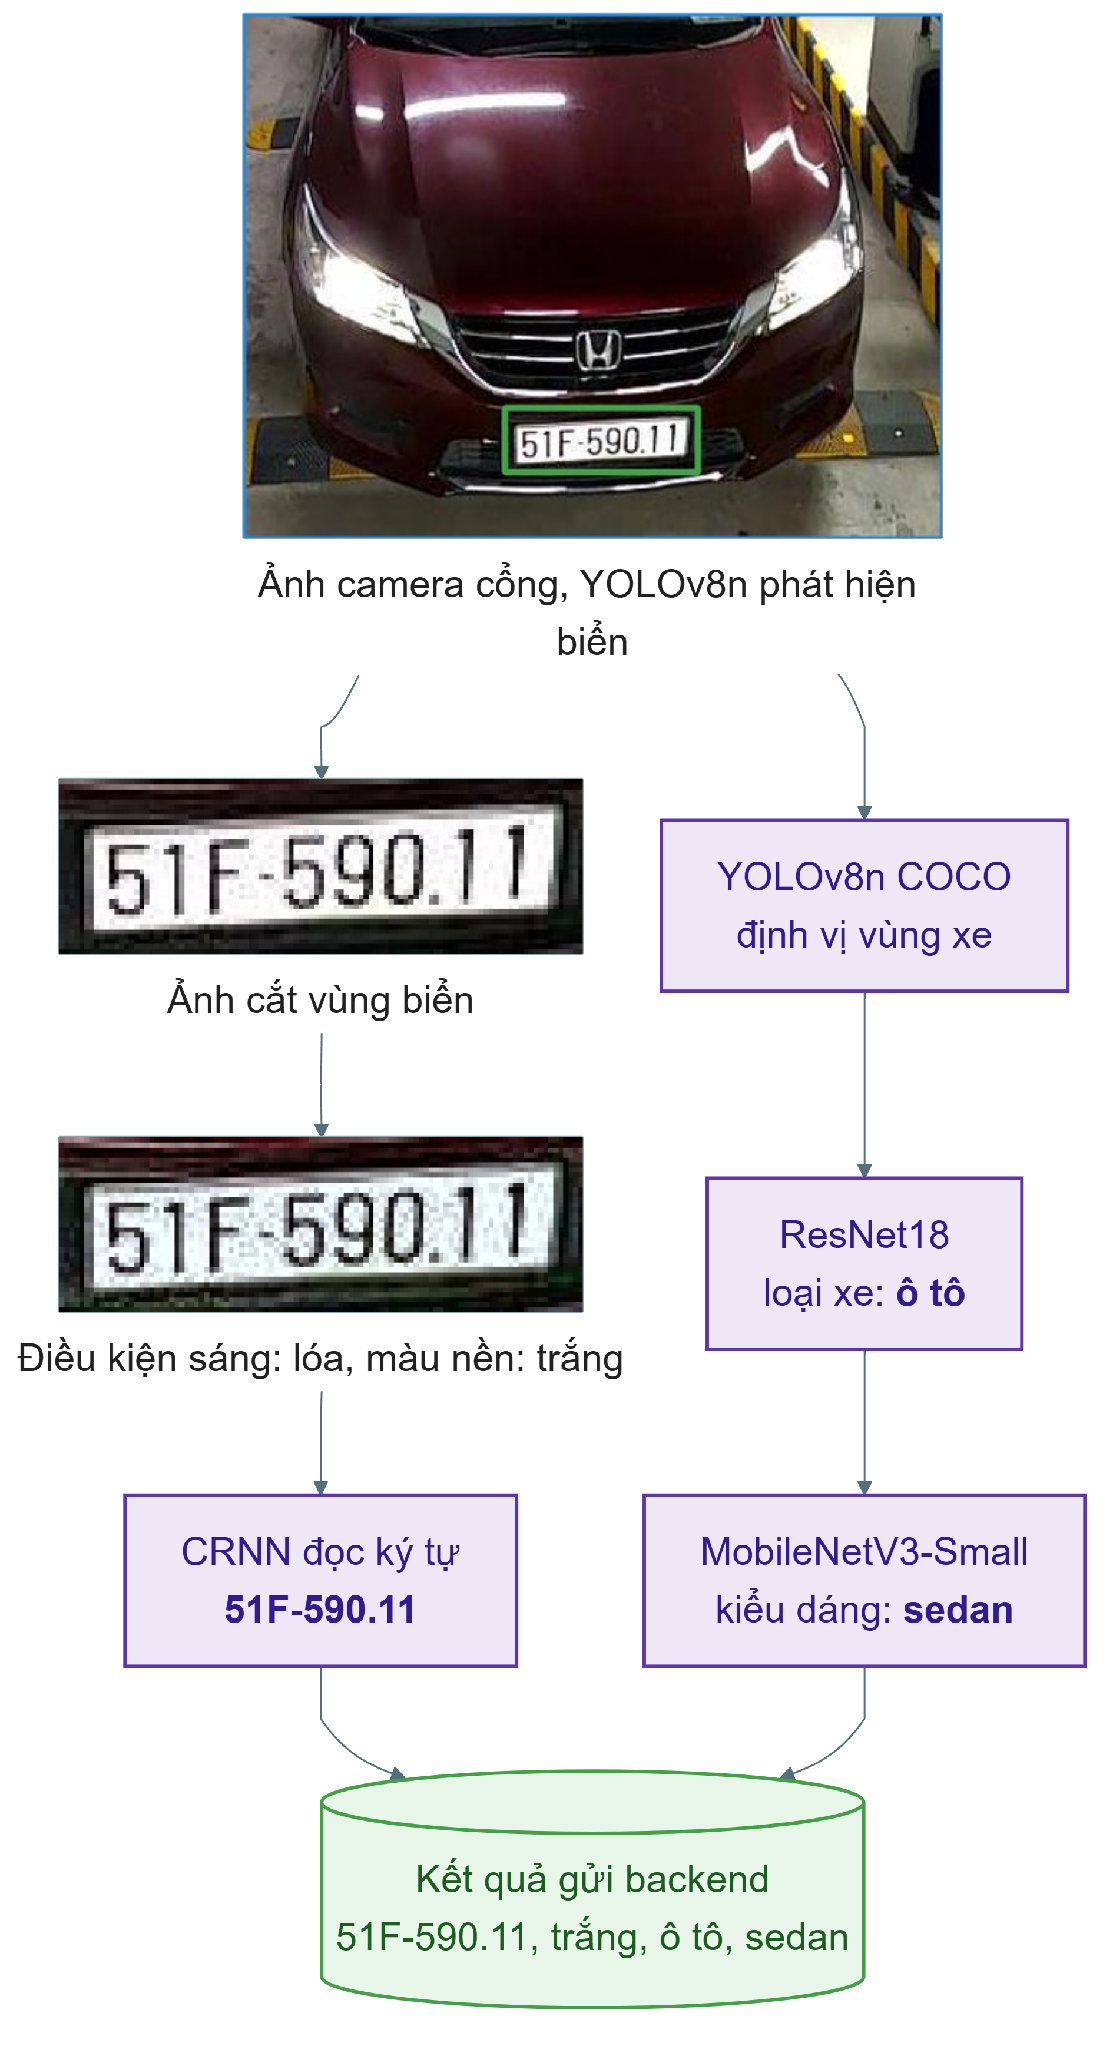
\includegraphics[width=0.5\textwidth]{pipeline-example.png}
\caption{Pipeline nhận diện minh họa trên một ảnh camera cổng thật: nhánh biển số (phát hiện biển, nhận màu nền, đọc ký tự) và nhánh xe (định vị vùng xe, phân loại loại xe bằng ResNet18, phân loại kiểu dáng bằng MobileNetV3-Small).}

\label{fig:pipeline}
\end{figure}

\section{Cấu Trúc Báo Cáo}

Chương~\ref{ch:lienquan} khảo sát các công trình liên quan và định vị khoảng trống của
đề tài. Chương~\ref{ch:dulieu} trình bày quy định biển số và dữ liệu.
Chương~\ref{ch:phathien}, \ref{ch:ocr} và \ref{ch:phanloai} lần lượt trình bày phát hiện
biển số, nhận dạng ký tự cùng màu nền biển, và phân loại phương tiện.
Chương~\ref{ch:hethong} mô tả hệ thống quản lý bãi xe, Chương~\ref{ch:trienkhai} đánh
giá triển khai trên Raspberry Pi 5, Chương~\ref{ch:ketluan} tổng kết và nêu hướng phát
triển.
      % Chương 1: Giới thiệu
% =====================================================================
%  CHƯƠNG 2. TỔNG QUAN CÔNG TRÌNH LIÊN QUAN       | Phụ trách: Cả 2
%  Ngân sách: mục tiêu 8 trang, trần 9 trang
%  Nguồn: docs/research/2026-07-18-yolo-architecture.md            (2.1),
%         docs/research/khao-sat-he-thong-alpr.md                  (2.2, 2.3),
%         docs/research/2026-07-19-similar-parking-systems.md      (2.4, 2.5)
% =====================================================================
\chapter{Tổng Quan Công Trình Liên Quan}
\label{ch:lienquan}

\section{Phát Hiện Đối Tượng và Họ Kiến Trúc YOLO}

\subsection{Đối Lập Một Giai Đoạn và Hai Giai Đoạn}

Các phương pháp phát hiện đối tượng (object detection) hai giai đoạn (two-stage) sinh
tập vùng đề xuất (region proposal) rồi phân loại và tinh chỉnh tọa độ từng vùng. Faster
R-CNN vẫn xử lý tuần tự theo vùng đề xuất nên chỉ đạt khoảng năm FPS trên GPU cùng
thời~\autocite{ren2015fasterrcnn}. Ngược lại, họ YOLO (You Only Look
Once) đưa phát hiện về một bài toán regression duy nhất: ảnh chia lưới, mạng dự đoán
trực tiếp bounding box và lớp trong một lần forward pass. YOLOv1 đạt 45 FPS với mAP gần
gấp đôi các detector real-time cùng thời, đánh đổi một phần độ chính xác định vị để lấy
tốc độ~\autocite{redmon2016yolo}. Đánh đổi này phù hợp ràng buộc thời gian thực trên CPU
không GPU: một detector hai giai đoạn chạy hai lần liên tiếp cho phát hiện xe rồi biển số
sẽ cộng dồn độ trễ tới mức khó đạt mục tiêu dưới hai giây.

\subsection{Kiến Trúc YOLOv8}
\label{sec:yolov8}

YOLOv8 đánh dấu bước chuyển kiến trúc quan trọng: bỏ hoàn toàn anchor box (anchor-free),
tách head detection thành hai nhánh song song (decoupled head) cho box regression và
class score, và dùng Task-Aligned Assigner khi gán nhãn huấn luyện. Backbone dùng block
C2f thay cho C3 của YOLOv5 để tái sử dụng đặc trưng phong phú hơn; neck PAN-FPN fuse
feature ba tỷ lệ. Mỗi anchor point regress bốn khoảng cách cạnh qua Distribution Focal
Loss (DFL) với 16 bin xác suất rời rạc thay vì một scalar, cải thiện định vị vật thể nhỏ
và mờ; điểm class sau sigmoid chính là confidence, không có nhánh objectness riêng. Sau
giải mã DFL, Non-Maximum Suppression (NMS) lọc các detection trùng lặp, là bước hậu xử lý
tuần tự nằm ngoài graph tensor, thêm độ trễ và phức tạp hóa xuất
ONNX~\autocite{jocher2023yolov8,terven2023comprehensive}.

\subsection{YOLO26: Thiết Kế Hướng Đến Edge và Xuất Mô Hình}
\label{sec:yolo26}

YOLO26, ra mắt tháng 1/2026 với paper arXiv công bố tháng 6/2026, được Ultralytics định
vị là thế hệ hiện tại cho deploy CPU và edge. Bốn thay đổi kiến trúc chính so với YOLOv8
được xác nhận từ abstract arXiv và docs chính
thức~\autocite{jocher2026yolo26,chakrabarty2026yolo26nmsfree}:

\begin{itemize}
  \item \textbf{NMS-free end-to-end:} dual-head cho phép train theo cách gán one-to-many thông thường nhưng export và chạy bằng head one-to-one xuất detection cuối trực tiếp, không cần bước NMS, đơn giản hóa graph ONNX và giảm latency deploy.
  \item \textbf{Bỏ DFL:} head không còn softmax 16-bin cho mỗi cạnh box, nên head nhẹ hơn và graph export INT8 đơn giản hơn vì loại op Softmax vốn khó lượng tử hóa trên NPU và DSP~\autocite{chakrabarty2026yolo26nmsfree}.
  \item \textbf{MuSGD:} optimizer lai SGD và Muon lấy cảm hứng từ huấn luyện mô hình ngôn ngữ lớn, cải thiện hội tụ.
  \item \textbf{Progressive Loss và STAL:} Progressive Loss dịch trọng tâm supervision về head one-to-one; STAL (Small-Target-Aware Label Assignment) đảm bảo độ phủ positive cho vật thể nhỏ, nhắm trực tiếp vào bài toán biển số nhỏ trong khung ảnh bãi đỗ.
\end{itemize}

Trên COCO val với input 640, YOLO26n đạt 40,9 mAP ở 38,9 ms CPU ONNX (Intel Xeon), còn
YOLOv8n đạt 37,3 mAP ở 80,4 ms cùng điều kiện.

Đề tài so sánh trực tiếp YOLOv8n và YOLO26n trên dữ liệu biển số Việt Nam ở
Chương~\ref{ch:phathien}.

\section{Nhận Dạng Biển Số Xe Tự Động}

\subsection{Kiến Trúc Ba Tầng trong ALPR}

Nhận dạng biển số xe tự động (Automatic License Plate Recognition, ALPR) thường gồm ba
tầng: phát hiện vùng biển, chuẩn hóa và tách dòng, rồi đọc ký tự bằng OCR hoặc theo hướng
OCR-as-detection (dùng detector YOLO phát hiện từng ký tự). Al-batat và cộng sự công bố
một pipeline ALPR mã nguồn mở đánh giá trên năm bộ dữ liệu nhiều khu vực (Mỹ, EU, Đài
Loan, Brazil), đạt 90,3\% ở cấp ký tự trung bình; khi đo từng tầng riêng, phát hiện xe
đạt 99,71\% precision và nhận dạng ký tự tách riêng đạt 99,68\%, cho thấy khoảng cách lớn
giữa kết quả từng tầng và kết quả toàn
pipeline~\autocite{albatat2022endtoend,redalb2022alprcode}.

Bằng chứng định lượng rõ nhất cho lợi ích kiến trúc đa tầng là so sánh trực tiếp của
Safran và cộng sự: đa tầng đạt 96,1\% trong khi single-stage chỉ 83,9\% trên cùng dữ liệu
và điều kiện, chênh hơn 12 điểm phần trăm~\autocite{safran2024multistage}. Hệ thống này
còn tích hợp web dashboard trực quan hóa trạng thái chiếm chỗ và luồng xe thời gian thực,
một trong số ít công trình kết hợp cả ALPR và dashboard.

Moussaoui và cộng sự dùng YOLOv8 kết hợp EasyOCR với tiền xử lý k-means, thresholding và
morphology, đạt 99\% phát hiện và 98\% ký tự trên tập nhỏ 270
ảnh~\autocite{moussaoui2024yolov8ocr}.

\subsection{Bộ Dữ Liệu Quốc Tế và Giới Hạn với Biển Số Việt Nam}

Các benchmark quốc tế cung cấp nền tảng so sánh nhưng không phản ánh đặc thù biển số Việt
Nam. CCPD (Chinese City Parking Dataset) gồm khoảng 290 nghìn ảnh chụp tại bãi xe Bắc
Kinh với đa dạng điều kiện ánh sáng, góc nghiêng và thời tiết, là benchmark bãi xe lớn
nhất tìm được~\autocite{xu2018ccpd}. UFPR-ALPR gồm 4500 ảnh từ 150 phương tiện tại Brazil
ở độ phân giải 1920×1080, xe và camera đều chuyển động, có gán nhãn vị trí từng ký
tự~\autocite{laroca2018ufpr}. Cả hai chỉ có biển một hàng của nước ngoài, không
có biển hai hàng và ký tự ``Đ'' của Việt Nam, nên không thể so sánh số tuyệt đối với đề
tài.

\section{Nghiên Cứu trên Biển Số Việt Nam}

\subsection{Các Công Trình Nhận Dạng Biển Số Việt Nam}

Trong nước, một số công trình xử lý trực tiếp bối cảnh gần với đề tài. Tran và Bui triển
khai SSD-MobileNetV2 phát hiện vùng biển kết hợp YOLOv8-nano nhận dạng ký tự trên
Raspberry Pi 4 Model B với camera 8 MP, đạt độ chính xác trung bình 95,68\% với thời gian
0,478 giây mỗi ảnh~\autocite{tran2025vietnamlpr}. Đây là một trong số ít công trình trong
nước đo cả độ chính xác lẫn thời gian trên phần cứng biên (số liệu thứ cấp, chưa tiếp cận
được bản đầy đủ), nhưng dừng ở khâu nhận dạng, không có quản lý phiên hay tính phí.

Dang và cộng sự đề xuất YOLO phát hiện xe, WPOD-NET trích vùng biển (xử lý tốt biển xiên
góc), rồi CRNN huấn luyện đồng thời với CTC loss và attention để đọc ký tự, đạt Word Error
Rate 0,014 trên dữ liệu tự thu tại bãi đỗ trong nhà ở Việt
Nam~\autocite{dang2024vietnamcrnn}. Ngữ cảnh sát bài toán của đề tài, nhưng cỡ tập test và
protocol đo không được công bố nên khó đánh giá độ tin cậy.

Với biển xe máy, Le và cộng sự đề xuất YOLOv8 ba tầng (phát hiện xe máy, phát hiện biển
trong bbox xe máy, nhận dạng biển), đạt mAP 93\% sau 300 epoch, cung cấp baseline trực
tiếp cho biển hai hàng, loại khó nhất trong bối cảnh đề tài~\autocite{le2023motorcycleplate}.
Các hướng khác gồm nhận dạng đa góc nhìn trên bộ PTITPlates~\autocite{trananh2023multiangle},
cuộc thi nhận dạng biển xe máy UIT MAPR 2018 với 3000 ảnh chụp tại bãi giữ
xe~\autocite{mapr2018challenge}, và dự án mã nguồn mở mrzaizai2k dùng KNN cùng OpenCV cho
cả biển một và hai hàng~\autocite{mrzaizai2k2025vnplate}.

\subsection{Đặc Điểm Chung và Khoảng Hở của Các Công Trình Việt Nam}

Tổng hợp cho thấy hai điểm chung: phần lớn dừng ở khâu nhận dạng biển số, không mở rộng
sang quản lý phiên hay tính phí; và không công trình nào đo hiệu năng trên Raspberry Pi 5
hoặc phần cứng tương đương trong điều kiện thực tế cổng bãi xe.

\section{Hệ Thống Quản Lý Bãi Giữ Xe}

\subsection{Các Hệ Thống Đại Diện}

Pradhan và cộng sự xây dựng bãi xe IoT trên Raspberry Pi 4 quản lý bốn camera, chạy YOLO
cùng Tesseract OCR với tiền xử lý OpenCV, tích hợp cảm biến IR và ESP32 cho mỗi ô đỗ, ghi
thời gian vào ra, tính phí động theo giờ cao và thấp điểm, theo dõi trạng thái chiếm chỗ.
Trên 100 test case: khớp biển tổng thể 88,9\%; theo điều kiện 95\% ban ngày, 90\% ánh
sáng yếu, 93\% góc 45°; sai số theo dõi chiếm chỗ dưới 5\% so với đếm thủ
công~\autocite{pradhan2025iotparking}. Đây là công trình tích hợp trọn vẹn nhất về thiết bị
biên, ALPR, phiên và tính phí, nhưng mỗi ô đỗ cần một ESP32 và cảm biến IR nên chi phí
phần cứng cao.

Ammar và cộng sự triển khai pipeline năm tầng tại cổng campus trên Jetson Xavier AGX:
YOLOv4 phát hiện xe và biển từ RTSP stream, Xception phân loại 196 đời xe, YOLOv4 nhận
dạng ký tự, DeepSORT theo dõi đa khung hình kèm voting, tối ưu bằng TensorRT, đạt 17,1 FPS
trung bình. Voting qua nhiều frame tăng độ chính xác biển đầy đủ từ 29\% (một frame) lên
69\% (tối đa 35 frame); độ phân giải camera quyết định kết quả: 80\% ở 1080p, 72\% ở
720p, chỉ 23\% ở 480p. Khoảng cách giữa validation cấp ký tự (99,8\%) và thực tế toàn
pipeline (74\%) cho thấy cần báo cáo cả hai cấp độ đo~\autocite{ammar2023multistage}.

Rani và cộng sự xây dựng hệ thống có quản lý vào ra và tính phí: module vào ghi biển và
timestamp, module ra tính phí theo thời lượng và sinh QR code động cho thanh toán không
tiếp xúc, đạt 97,11\% LPR khi không tính khoảng trắng và 91,91\% khi tính cả khoảng
trắng, minh họa mức phụ thuộc của kết quả vào quy tắc chuẩn hóa
chuỗi~\autocite{rani2024ips}. Arukonda và cộng sự dùng YOLOv8 kết hợp EasyOCR và Tesseract
với bước validate định dạng biển theo quy tắc quốc gia, đạt 98,5\% detect, latency 50 ms
mỗi frame (phần cứng không nêu), nhưng backend chỉ ghi log Excel chứ không có cơ sở dữ
liệu thực~\autocite{arukonda2026smartparking}.

\subsection{So Sánh Các Hệ Thống Bãi Giữ Xe}

Bảng~\ref{tab:parking-compare} so sánh các hệ thống trên theo chức năng và nền tảng triển
khai.

\begin{table}[htbp]
\centering
\caption{So sánh các hệ thống quản lý bãi giữ xe tiêu biểu.}

\footnotesize Nguồn: tổng hợp từ \autocite{pradhan2025iotparking,ammar2023multistage,safran2024multistage,rani2024ips,arukonda2026smartparking,platerecognizer2026alpr,openalpr2016benchmarks}.
\label{tab:parking-compare}
\begin{tabular}{p{3.0cm} p{2.4cm} p{1.9cm} p{1.7cm} p{1.4cm} p{1.5cm}}
\hline
\textbf{Hệ thống} & \textbf{Nền tảng} & \textbf{Phát hiện biển} & \textbf{Quản lý session} & \textbf{Dashboard} & \textbf{Màu biển} \\
\hline
Pradhan 2025~\autocite{pradhan2025iotparking}
  & Raspberry Pi 4
  & 88,9\% (n=100)
  & Có (tính phí động)
  & Không
  & Không \\
Ammar 2023~\autocite{ammar2023multistage}
  & Jetson Xavier AGX
  & 74\% (video)
  & Không
  & Không
  & Không \\
Safran 2024~\autocite{safran2024multistage}
  & Server
  & 96,1\%
  & Không
  & Có (web)
  & Không \\
Rani 2024~\autocite{rani2024ips}
  & PC
  & 97,1\%
  & Có (QR thanh toán)
  & Không
  & Không \\
Arukonda 2026~\autocite{arukonda2026smartparking}
  & Không rõ
  & 98,5\%
  & Không
  & Không
  & Không \\
Plate Recognizer~\autocite{platerecognizer2026alpr}
  & SDK on-prem (Pi, Jetson)
  & Không công bố
  & Có (ParkPow)
  & Có (ParkPow)
  & Màu xe \\
Rekor Scout~\autocite{openalpr2016benchmarks}
  & Server và edge agent
  & Không công bố
  & Không
  & Có (cloud)
  & Màu xe \\
\textbf{Đề tài này}
  & \textbf{Raspberry Pi 5}
  & \textbf{Mục tiêu >90\%}
  & \textbf{Có (CSDL, tính phí)}
  & \textbf{Có (React)}
  & \textbf{Màu nền biển} \\
\hline
\end{tabular}
\end{table}

Ngoài đề tài này, không hệ thống nào nhận màu nền biển; Plate Recognizer và Rekor Scout chỉ
nhận màu xe. Về deploy, chỉ Pradhan 2025 và đề tài này chạy trên phần cứng edge
Raspberry Pi; các hệ thống còn lại dùng máy chủ riêng hoặc cloud. Về nghiệp vụ, không
công trình học thuật nào khảo sát tích hợp đầy đủ ALPR, session với đối chiếu chống gian
lận, tính phí và dashboard trên một thiết bị biên duy nhất.

\section{Trí Tuệ Nhân Tạo trên Thiết Bị Biên}

\subsection{Nén Mô Hình và Lượng Tử Hóa}

Triển khai suy luận trên thiết bị biên đòi hỏi nén mô hình (model compression) cho phù
hợp bộ nhớ và năng lực tính toán hạn chế. Lượng tử hóa INT8 (quantization) là kỹ thuật
phổ biến nhất: biểu diễn trọng số và kích hoạt từ dấu phẩy động 32-bit (FP32) về số
nguyên 8-bit, giảm bộ nhớ và tăng tốc tính toán nhờ phép nhân nguyên hiệu quả, đổi lại
một phần nhỏ độ chính xác.

Sonnara và cộng sự với kiến trúc Light-Edge (backbone ResNet-18 cùng FPN, head
anchor-free, head nhận dạng CTC) cho thấy lượng tử hóa INT8 qua TensorRT tăng
throughput 4,6 lần từ 3,1 FPS lên 14,2 FPS trên Jetson Nano với input 1280×720, chỉ mất
0,4 điểm phần trăm mAP (từ 90,6\% xuống 90,2\%) nhờ giữ lớp đầu và lớp cuối ở FP16 (lượng
tử hóa hỗn hợp)~\autocite{sonnara2025lightedge}. Jetson Nano và Pi 5 khác lớp phần cứng nên con số
này không chuyển trực tiếp sang Pi 5 được.

Chakrabarty chỉ ra lớp Softmax của DFL khó lượng tử hóa trên NPU và DSP, nên việc YOLO26
bỏ DFL (Mục~\ref{sec:yolo26}) thuận lợi hơn cho INT8~\autocite{chakrabarty2026yolo26nmsfree};
lợi ích này trên Pi 5 với ONNX Runtime vẫn cần đo thực tế.

\subsection{Raspberry Pi 5 và Benchmark Thiết Bị Biên}
\label{sec:pi5bench}

Raspberry Pi 5 với CPU ARM Cortex-A76, ra mắt cuối 2023, là thế hệ tiến bộ đáng kể so với
Pi 4. Hướng dẫn chính thức của Ultralytics báo cáo YOLO26n trên Pi 5 ở 130,33 ms qua ONNX
Runtime và 67,69 ms qua NCNN FP32 với input 640×640~\autocite{ultralytics2026rpiguide}.
Với cascade hai lần detect (xe rồi biển số trên crop), tổng thời gian detection ước tính
khoảng 260 ms qua ONNX, để lại hơn 1,5 giây trong ngân sách 2 giây cho OCR, phân loại màu
và vào ra, nên detection không phải điểm nghẽn chính trên Pi 5 ở FP32. Benchmark đa SBC
xác nhận biến thể nano và small cho hiệu năng tốt nhất trên SBC và các mô hình YOLO
thường chiếm 4 đến 12\% RAM khả dụng trên Pi 4/5~\autocite{mdpi2026sbcbenchmark}, là cơ sở
để đề tài chọn Pi 5 làm nền tảng biên minh họa với biến thể nano cho cả hai detector.

\section{Khoảng Trống Nghiên Cứu và Định Vị Đề Tài}

\subsection{Hai Khoảng Trống Chính}

\textbf{Khoảng trống 1: Chưa hệ thống nào tích hợp trọn vẹn trên một thiết bị biên.}
Bảng~\ref{tab:parking-compare} cho thấy không công trình học thuật hay sản phẩm thương mại
nào kết hợp đồng thời ALPR, backend nghiệp vụ (cơ sở dữ liệu, session vào ra, đối chiếu
chống gian lận, tính phí) và dashboard quản lý trên một thiết bị biên duy nhất. Pradhan
2025 gần nhất về tích hợp nhưng vẫn dùng máy chủ ngoài cho SQL Server và không có dashboard
web; Safran 2024 có dashboard nhưng chạy trên server. Vận hành mọi thành phần trên một Pi
5 buộc suy luận, backend và cơ sở dữ liệu chia sẻ cùng tài
nguyên~\autocite{pradhan2025iotparking,ammar2023multistage}.

\textbf{Khoảng trống 2: Màu nền biển số chưa được khai thác như tín hiệu phân loại.} Tại
Việt Nam, màu nền biển mang giá trị pháp lý, phân biệt xe cá nhân, xe kinh doanh, xe cơ
quan nhà nước và xe quân sự (Mục~\ref{sec:maunenbien}). Thông tin này cho phép phân nhóm phương
tiện ngay từ tầng thị giác mà không cần tra cứu cơ sở dữ liệu ngoài, hỗ trợ áp biểu phí
theo nhóm và phát hiện bất thường. Tuy nhiên không hệ thống nào trong khảo sát dùng tín
hiệu này.

\subsection{Định Vị Đề Tài}

Đề tài lấp hai khoảng trống này bằng pipeline nhận diện năm thành phần
(Mục~\ref{sec:donggop}) gắn với backend nghiệp vụ và dashboard, toàn bộ vận hành được trên
một Raspberry Pi 5.
       % Chương 2: Tổng quan công trình liên quan
% =====================================================================
%  CHƯƠNG 3. DỮ LIỆU                              | Phụ trách: Cả 2
%  Ngân sách: mục tiêu 9 trang, trần 10 trang
%  Nguồn: docs/research/quy-dinh-bien-so-xe-vn.md            (mục 3.1),
%         src/ml/notebooks/eda-plate-datasets.ipynb           (mục 3.2),
%         docs/research/eda_outputs/eda_summary.csv           (Bảng 3.4),
%         data/processed/a1_det/phash_report.txt              (mục 3.5)
% =====================================================================
\chapter{Dữ Liệu}
\label{ch:dulieu}

% =====================================================================
\section{Quy Định Biển Số Xe Việt Nam}
\label{sec:quydinhbienso}
% =====================================================================

Cấu trúc pháp lý của biển số quyết định cách thiết kế nhãn dữ liệu, bộ ký tự OCR và quy
tắc hậu xử lý.

\subsection{Căn Cứ Pháp Lý Hiện Hành}

Quy định biển số hiện hành (từ 01/01/2025) gồm Luật Trật tự, an toàn giao thông đường bộ
2024, lần đầu đưa màu nền biển vào luật, cùng ba Thông tư của Bộ Công an: 79/2024 về bộ
seri, số ký tự và kích thước theo loại xe (thay Thông tư 58/2020), 81/2024 ban hành quy
chuẩn QCVN 08:2024/BCA về kích thước và chất liệu biển, và 24/2023 quản lý biển theo mã
định danh chủ xe (biển gắn theo chủ, không theo
xe)~\autocite{luatttatgt2024,tt792024bca,tt812024bca,tt242023bca}.

\subsection{Cấu Trúc Chuỗi Ký Tự}

Định dạng tổng quát của biển số xe cơ giới Việt Nam là:

\begin{center}
\texttt{[Mã tỉnh 2 chữ số][gạch ngang][Seri 1 chữ cái] [Số thứ tự 5 chữ số, nhóm 3.2]}
\end{center}

\noindent Ví dụ biển một dòng (ô tô) \texttt{30A-123.45}; biển hai dòng (xe máy) dòng
trên \texttt{59N}, dòng dưới \texttt{187.51}. Ba thành phần có hệ quả trực tiếp với thiết
kế OCR:

\begin{itemize}
  \item \textbf{Mã tỉnh}: 2 chữ số từ 11 đến 99. Từ 01/07/2025, cả nước sáp nhập từ 63
        xuống 34 tỉnh thành (Thông tư 51/2025/TT-BCA), nhưng xe đăng ký trước đó giữ biển
        cũ, nên nhiều mã tỉnh cũ vẫn lưu hành song song nhiều năm.
  \item \textbf{Seri}: chọn trong tập \textbf{20 chữ cái} (A, B, C, D, E, F, G, H, K, L,
        M, N, P, S, T, U, V, X, Y, Z); sáu chữ I, J, O, Q, R, W không dùng cho biển dân
        sự. Bộ 20 chữ cái này được dùng để ràng buộc hậu xử lý OCR, loại nhầm lẫn O với 0
        và I với 1.
  \item \textbf{Số thứ tự}: 5 chữ số nhóm 3.2, từ 000.01 đến 999.99. Riêng seri MĐ và TĐ
        của xe máy điện chứa thêm ký tự ``Đ''.
\end{itemize}

\subsection{Bố Cục Biển Theo Loại Xe}

Biển dài một dòng và biển ngắn hai dòng không phải hai kiểu thay thế nhau: với ô tô, đây
là hai biển bắt buộc gắn đồng thời trên cùng một xe (Bảng~\ref{tab:bienso-bocuc}).

\begin{table}[htbp]
\centering
\caption{Bố cục biển số theo loại phương tiện.}

{\footnotesize Nguồn: \autocite{tt792024bca,tt812024bca}.}
\label{tab:bienso-bocuc}
\small
\begin{tabular}{p{3.2cm} p{1.6cm} p{3.0cm} p{3.0cm}}
\toprule
\textbf{Loại xe} & \textbf{Số biển} & \textbf{Bố cục} & \textbf{Kích thước (mm)} \\
\midrule
Ô tô (con, tải, khách) & 2 biển & Biển trước: 1 dòng 520$\times$110; biển sau: 2 dòng 330$\times$165 & 2 kích thước khác nhau \\
\addlinespace
Mô tô, xe gắn máy (kể cả xe máy điện) & 1 biển (sau) & Luôn 2 dòng & 190$\times$140 \\
\addlinespace
Máy kéo, rơ-moóc & 1 biển (sau) & 2 dòng & 330$\times$165 \\
\bottomrule
\end{tabular}
\end{table}

Hệ quả cho pipeline: camera cổng có thể thu biển một dòng hoặc hai dòng của cùng một ô tô
tùy góc đặt (trước hay sau xe), nên dữ liệu huấn luyện cần cân bằng cả hai bố cục.

\subsection{Màu Nền Biển và Ý Nghĩa Phân Loại Phí}
\label{sec:maunenbien}

Màu nền biển phản ánh nhóm chủ sở hữu theo pháp luật và là cơ sở áp biểu phí
(Chương~\ref{ch:hethong}). Bảng~\ref{tab:maubienso} tổng hợp bốn màu chính theo Luật Trật
tự, an toàn giao thông đường bộ 2024~\autocite{luatttatgt2024}.

\begin{table}[htbp]
\centering
\caption{Màu nền biển số xe và nhóm chủ sở hữu theo quy định hiện hành.}

{\footnotesize Nguồn: \autocite{luatttatgt2024,tt792024bca}.}
\label{tab:maubienso}
\begin{tabular}{p{2.2cm} p{4.8cm} p{3.6cm}}
\toprule
\textbf{Màu nền} & \textbf{Đối tượng} & \textbf{Ưu tiên đề tài} \\
\midrule
Trắng (chữ đen) & Cá nhân, tổ chức dân sự trong nước & Bắt buộc (chiếm đa số) \\
Vàng (chữ đen) & Xe kinh doanh vận tải: taxi, xe khách, xe tải kinh doanh & Bắt buộc \\
Xanh dương (chữ trắng) & Cơ quan Đảng, Nhà nước, đơn vị sự nghiệp công lập & Tùy chọn \\
Đỏ (chữ trắng) & Xe quân sự (Bộ Quốc phòng) & Tùy chọn \\
\bottomrule
\end{tabular}
\end{table}

Xe điện không có màu biển riêng, chỉ dán thêm tem nhận diện màu xanh lá. Màu thực tế trên
ảnh camera có thể lệch so với chuẩn CIE, đặc biệt dưới đèn flash hồng ngoại ban đêm, nên
cần xử lý CLAHE trước khi phân loại màu biển (Chương~\ref{ch:ocr}).

% =====================================================================
\section{Khảo Sát Bộ Dữ Liệu Công Khai}
\label{sec:khaosatdataset}
% =====================================================================

Đề tài khảo sát các bộ dữ liệu công khai theo hai nhóm: (A) biển số Việt Nam
(Bảng~\ref{tab:dataset-a}) và (B) phương tiện và bối cảnh Việt Nam
(Bảng~\ref{tab:dataset-b}); mỗi bộ được kiểm tra trực tiếp trên trang nguồn trong tháng 7
năm 2026. Các bộ ALPR và bãi xe nước ngoài như CCPD, PKLot, CNRPark+EXT, AOLP và OpenALPR
benchmarks~\autocite{xu2018ccpd,almeida2015pklot,amato2017cnrpark,hsu2013aolp,openalpr2016benchmarks}
chỉ dùng để đối chiếu vì không có biển số Việt Nam.

\subsection{Nhóm A: Biển Số Việt Nam}

\begin{table}[htbp]
\centering
\caption{Các bộ dữ liệu nhóm A: biển số xe Việt Nam.}

{\footnotesize Nguồn: Kaggle, Roboflow Universe.}
\label{tab:dataset-a}
\small
\begin{tabular}{p{0.8cm} p{3.2cm} p{1.4cm} p{1.6cm} p{1.6cm} p{2.0cm}}
\toprule
\textbf{Ký hiệu} & \textbf{Tên bộ dữ liệu} & \textbf{Host} & \textbf{Số ảnh} & \textbf{Giấy phép} & \textbf{Biển 1 hàng/2 hàng} \\
\midrule
A1 & Vietnam License Plate Segment (duydieunguyen)~\autocite{duydieunguyen2023vnplatesegment} & Kaggle & khoảng 5.000 & Không rõ & Có, tách rõ số lượng \\
A2 & Vietnamese Car License Plate (Cuong Ta)~\autocite{cuongta2021vnplate} & Roboflow & 8.255 & CC0 1.0 & Không rõ tỷ lệ \\
A3 & vietnamese-license-plate-tptd0 (school-fuhih)~\autocite{schoolfuhih2023vnplate} & Roboflow & 8.397 & CC BY 4.0 & Không rõ tỷ lệ \\
A4 & Motorcycle License Plate (HaUI)~\autocite{haui2023motorcycleplate} & Roboflow & 1.748 & MIT & Thiên về xe máy (2 hàng) \\
A5 & greenParking (thaiphung) & Roboflow & 1.748 & CC BY 4.0 & Không xác định \\
A6 & Viet Nam OCR plate (license-plate-reg)~\autocite{licenseplatereg2025ocrplate} & Roboflow & 3.819 & CC0 1.0 & Không rõ tỷ lệ \\
A7 & VNLicensePlate\_yolov7 (bomaich)~\autocite{bomaich2022vnlicenseplate7} & Kaggle & 1.000 & Không rõ & Có, không tách số \\
\bottomrule
\end{tabular}
\end{table}

Không bộ nào trong nhóm A ghi rõ điều kiện ánh sáng hay bối cảnh chụp.

\subsection{Nhóm B: Phương Tiện và Bối Cảnh Đường Phố Việt Nam}

\begin{table}[htbp]
\centering
\caption{Các bộ dữ liệu nhóm B: phương tiện và bối cảnh Việt Nam.}

{\footnotesize Nguồn: Roboflow Universe, GitHub.}
\label{tab:dataset-b}
\small
\begin{tabular}{p{0.8cm} p{3.4cm} p{1.4cm} p{1.3cm} p{1.4cm} p{2.5cm}}
\toprule
\textbf{Ký hiệu} & \textbf{Tên bộ dữ liệu} & \textbf{Host} & \textbf{Số ảnh} & \textbf{Giấy phép} & \textbf{Ghi chú} \\
\midrule
B1 & Vietnamese vehicle v3 (car-classification)~\autocite{carclassification2023vnvehicle} & Roboflow & 1.547 & CC BY 4.0 & 4 lớp gốc car/bus/truck/motorcycle, đã được ánh xạ lại thành 8 lớp \\
B2 & Vehicle Vietnam-CanTho~\autocite{vehicle2022cantho} & Roboflow & 1.110 đến 1.746 & CC BY 4.0 & Chỉ ban ngày, đường phố Cần Thơ \\
B3 & UIT-CVID21~\autocite{uitcvid21} & GitHub (UIT) & 10.000 (chưa xem được thật) & Không rõ & Chụp từ drone, khác góc camera cổng bãi xe \\
B4 & QuangTranUTE/Vehicle-Detection & GitHub & khoảng 11.000 & Không rõ & Camera giám sát giao thông, không phải bãi xe \\
B5 & Vehicle Body Style Dataset~\autocite{researchprojects2022vehiclebodystyle} & Roboflow & 10.000 & CC BY 4.0 & 12 kiểu dáng theo phân loại CompCars, gốc Trung Quốc \\
\bottomrule
\end{tabular}
\end{table}

Chưa bộ dữ liệu Việt Nam nào ở nhóm B tách phương tiện theo kiểu dáng thân xe (sedan, SUV,
pickup), nên đề tài bổ sung B5. B5 có 12 lớp gần cân bằng (lớp lớn nhất chỉ gấp 1,02 lần lớp nhỏ
nhất), nhưng xe chiếm trung bình 0,31 diện tích ảnh và không có xe máy, phản ánh phong cách
chụp tại đại lý, khác ảnh camera cổng; hạn chế này được phân tích ở
Chương~\ref{ch:phanloai}.

\subsection{Đánh Giá và Hướng Lựa Chọn}
\label{sec:chondataset}

Đề tài chọn A1 làm bộ chính cho phát hiện biển vì là bộ duy nhất tách rõ biển một hàng
(BSD) và biển hai hàng (BSV). A1 cùng A3 và A4 được tải về và phân tích khám phá ở
Mục~\ref{sec:edabienso} để xác minh bối cảnh chụp.

% =====================================================================
\section{Phân Tích Khám Phá Dữ Liệu Biển Số}
\label{sec:edabienso}
% =====================================================================

Ba bộ A1, A3, A4 được tải và phân tích khám phá độc lập, kết quả tổng hợp ở
Bảng~\ref{tab:eda-summary}.

\subsection{Tổng Quan Số Liệu}

\begin{table}[htbp]
\centering
\caption{Tổng hợp kết quả EDA trên ba bộ dữ liệu biển số được chọn.}

{\footnotesize Độ sáng đo trên mẫu ngẫu nhiên $n = 600$ ảnh mỗi bộ, seed cố định 42.}
\label{tab:eda-summary}
\begin{tabular}{lrrp{3.4cm}rr}
\toprule
\textbf{Bộ dữ liệu} & \textbf{Số ảnh} & \textbf{Số object} & \textbf{Độ phân giải (px)} & \textbf{Độ sáng TB} & \textbf{\% ảnh tối} \\
\midrule
A3 & 8.357 & 8.548 & 640$\times$640 (cố định) & 100,7 & 12,8\% \\
A4 & 1.748 & 1.748 & 472$\times$303 (cố định) & 111,1 & 0,0\% \\
A1 & 4.578 & 5.200 & 380 đến 4032 $\times$ 285 đến 3024 & 102,1 & 10,7\% \\
\bottomrule
\end{tabular}
\end{table}

\subsection{Phân Bố Lớp và Kích Thước Biển Số}

Hình~\ref{fig:eda-class} cho thấy ở A1, lớp BSV (biển hai hàng, 3.559 đối tượng) nhiều gấp
khoảng 2,2 lần lớp BSD (biển một hàng, 1.641 đối tượng); nếu gộp ba bộ để huấn luyện cần
xử lý mất cân bằng này để mô hình không thiên về biển hai hàng.

\begin{figure}[htbp]
\centering

\includegraphics[width=0.90\textwidth]{eda_class_distribution.png}
\caption{Phân bố số lượng object gán nhãn theo bộ dữ liệu và theo lớp (BSD và BSV).}

\label{fig:eda-class}
\end{figure}

Tỷ lệ diện tích vùng biển trên toàn ảnh trung bình chỉ khoảng
0,028 đến 0,043 ở cả ba bộ (Hình~\ref{fig:eda-arearatio}): phần lớn ảnh chụp toàn cảnh đầu
xe chứ không cận cảnh sát biển, đúng đặc thù camera cổng bãi xe.

\begin{figure}[htbp]
\centering
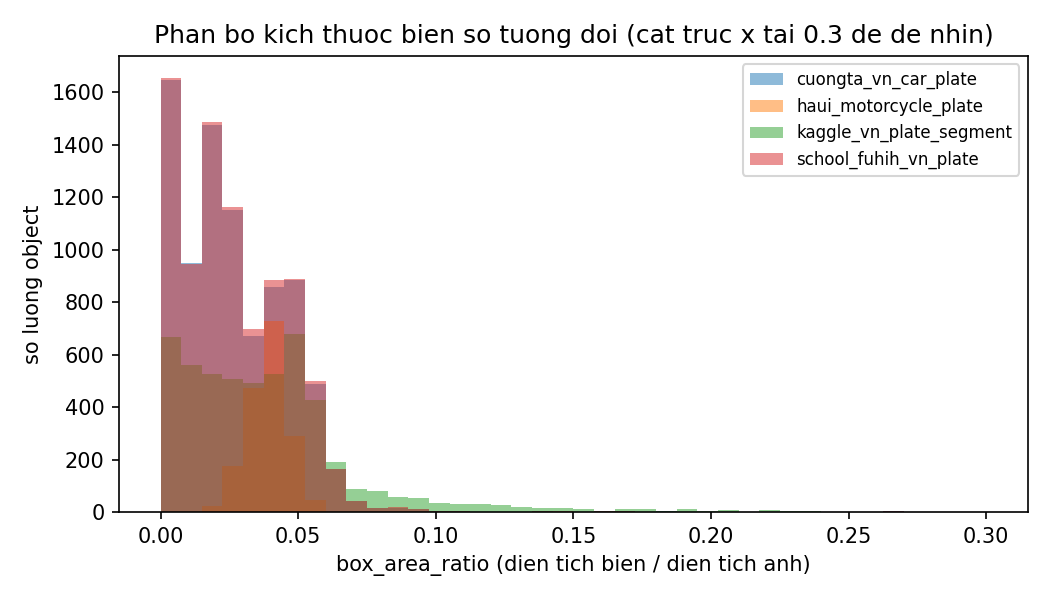
\includegraphics[width=0.90\textwidth]{eda_plate_area_ratio.png}
\caption{Phân bố tỷ lệ diện tích biển số trên diện tích ảnh cho ba bộ dữ liệu.}

\label{fig:eda-arearatio}
\end{figure}

\subsection{Kích Thước Ảnh và Độ Sáng}

A3 và A4 đã bị Roboflow resize về kích thước cố định khi xuất (640$\times$640 và
472$\times$303, độ lệch chuẩn bằng không) nên độ phân giải gốc coi như mất; chỉ A1 tải
trực tiếp từ Kaggle còn giữ kích thước gốc, rộng từ 380 đến 4032 pixel
(Hình~\ref{fig:eda-size}). Do không bộ nào có nhãn ánh sáng, độ sáng trung bình ảnh xám
(thang 0 đến 255) được dùng làm proxy tạm: A4 gần như không biến thiên, A3 và A1 có khoảng
11 đến 13\% ảnh ở mức tối.

\begin{figure}[htbp]
\centering
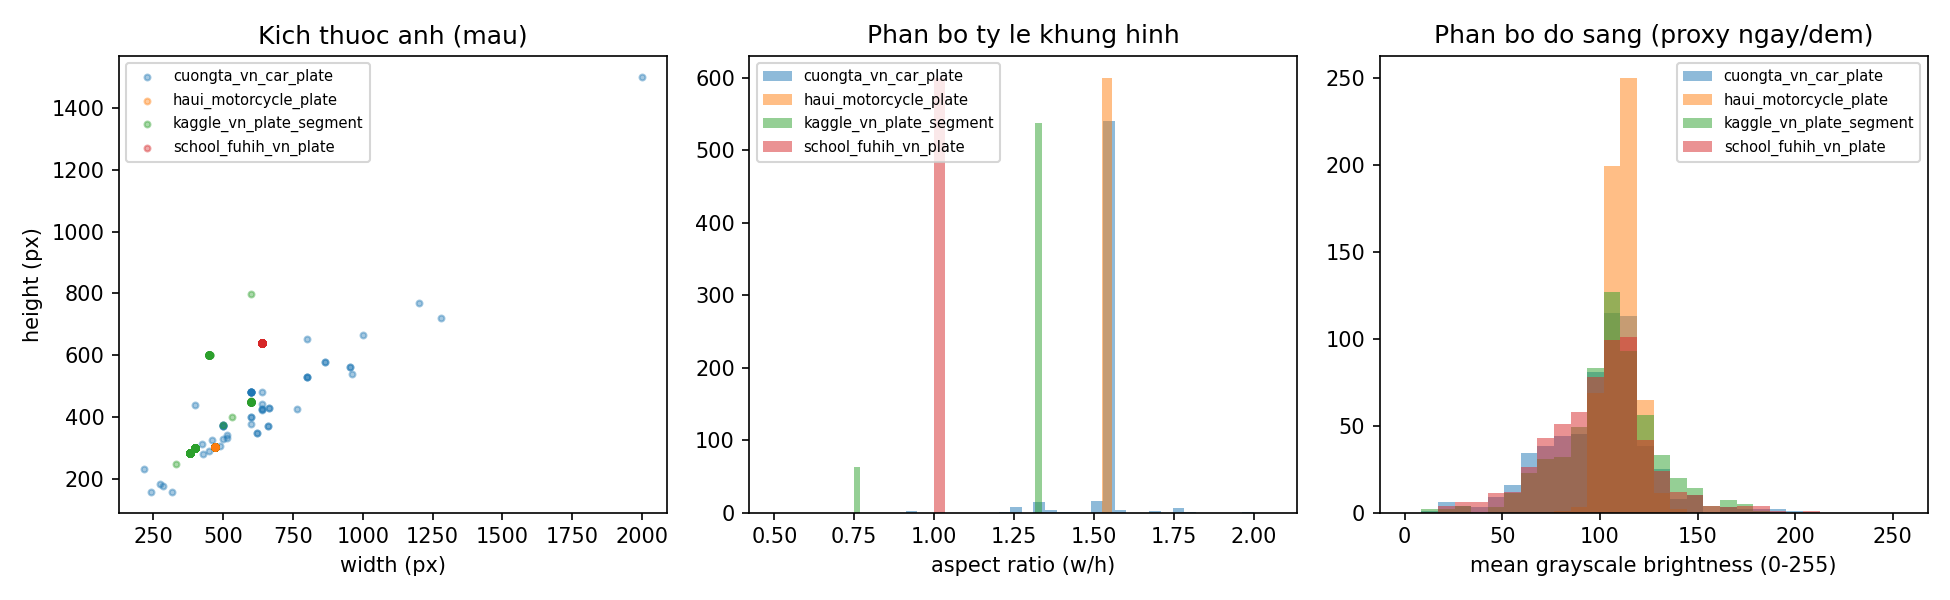
\includegraphics[width=0.90\textwidth]{eda_size_brightness.png}
\caption{Phân bố kích thước ảnh, tỷ lệ khung hình và độ sáng trên ba bộ dữ liệu.}

\label{fig:eda-size}
\end{figure}

\subsection{Xem Mẫu Ảnh để Xác Minh Bối Cảnh}

Ảnh mẫu (Hình~\ref{fig:eda-sample}) cho thấy cả ba bộ đều chụp từ camera cổng bãi xe hoặc
hầm gửi xe, có thanh chắn trong khung, nhiều ảnh có timestamp kiểu camera DVR và ảnh hầm
thiếu sáng, đúng bối cảnh đề tài.

\begin{figure}[htbp]
\centering
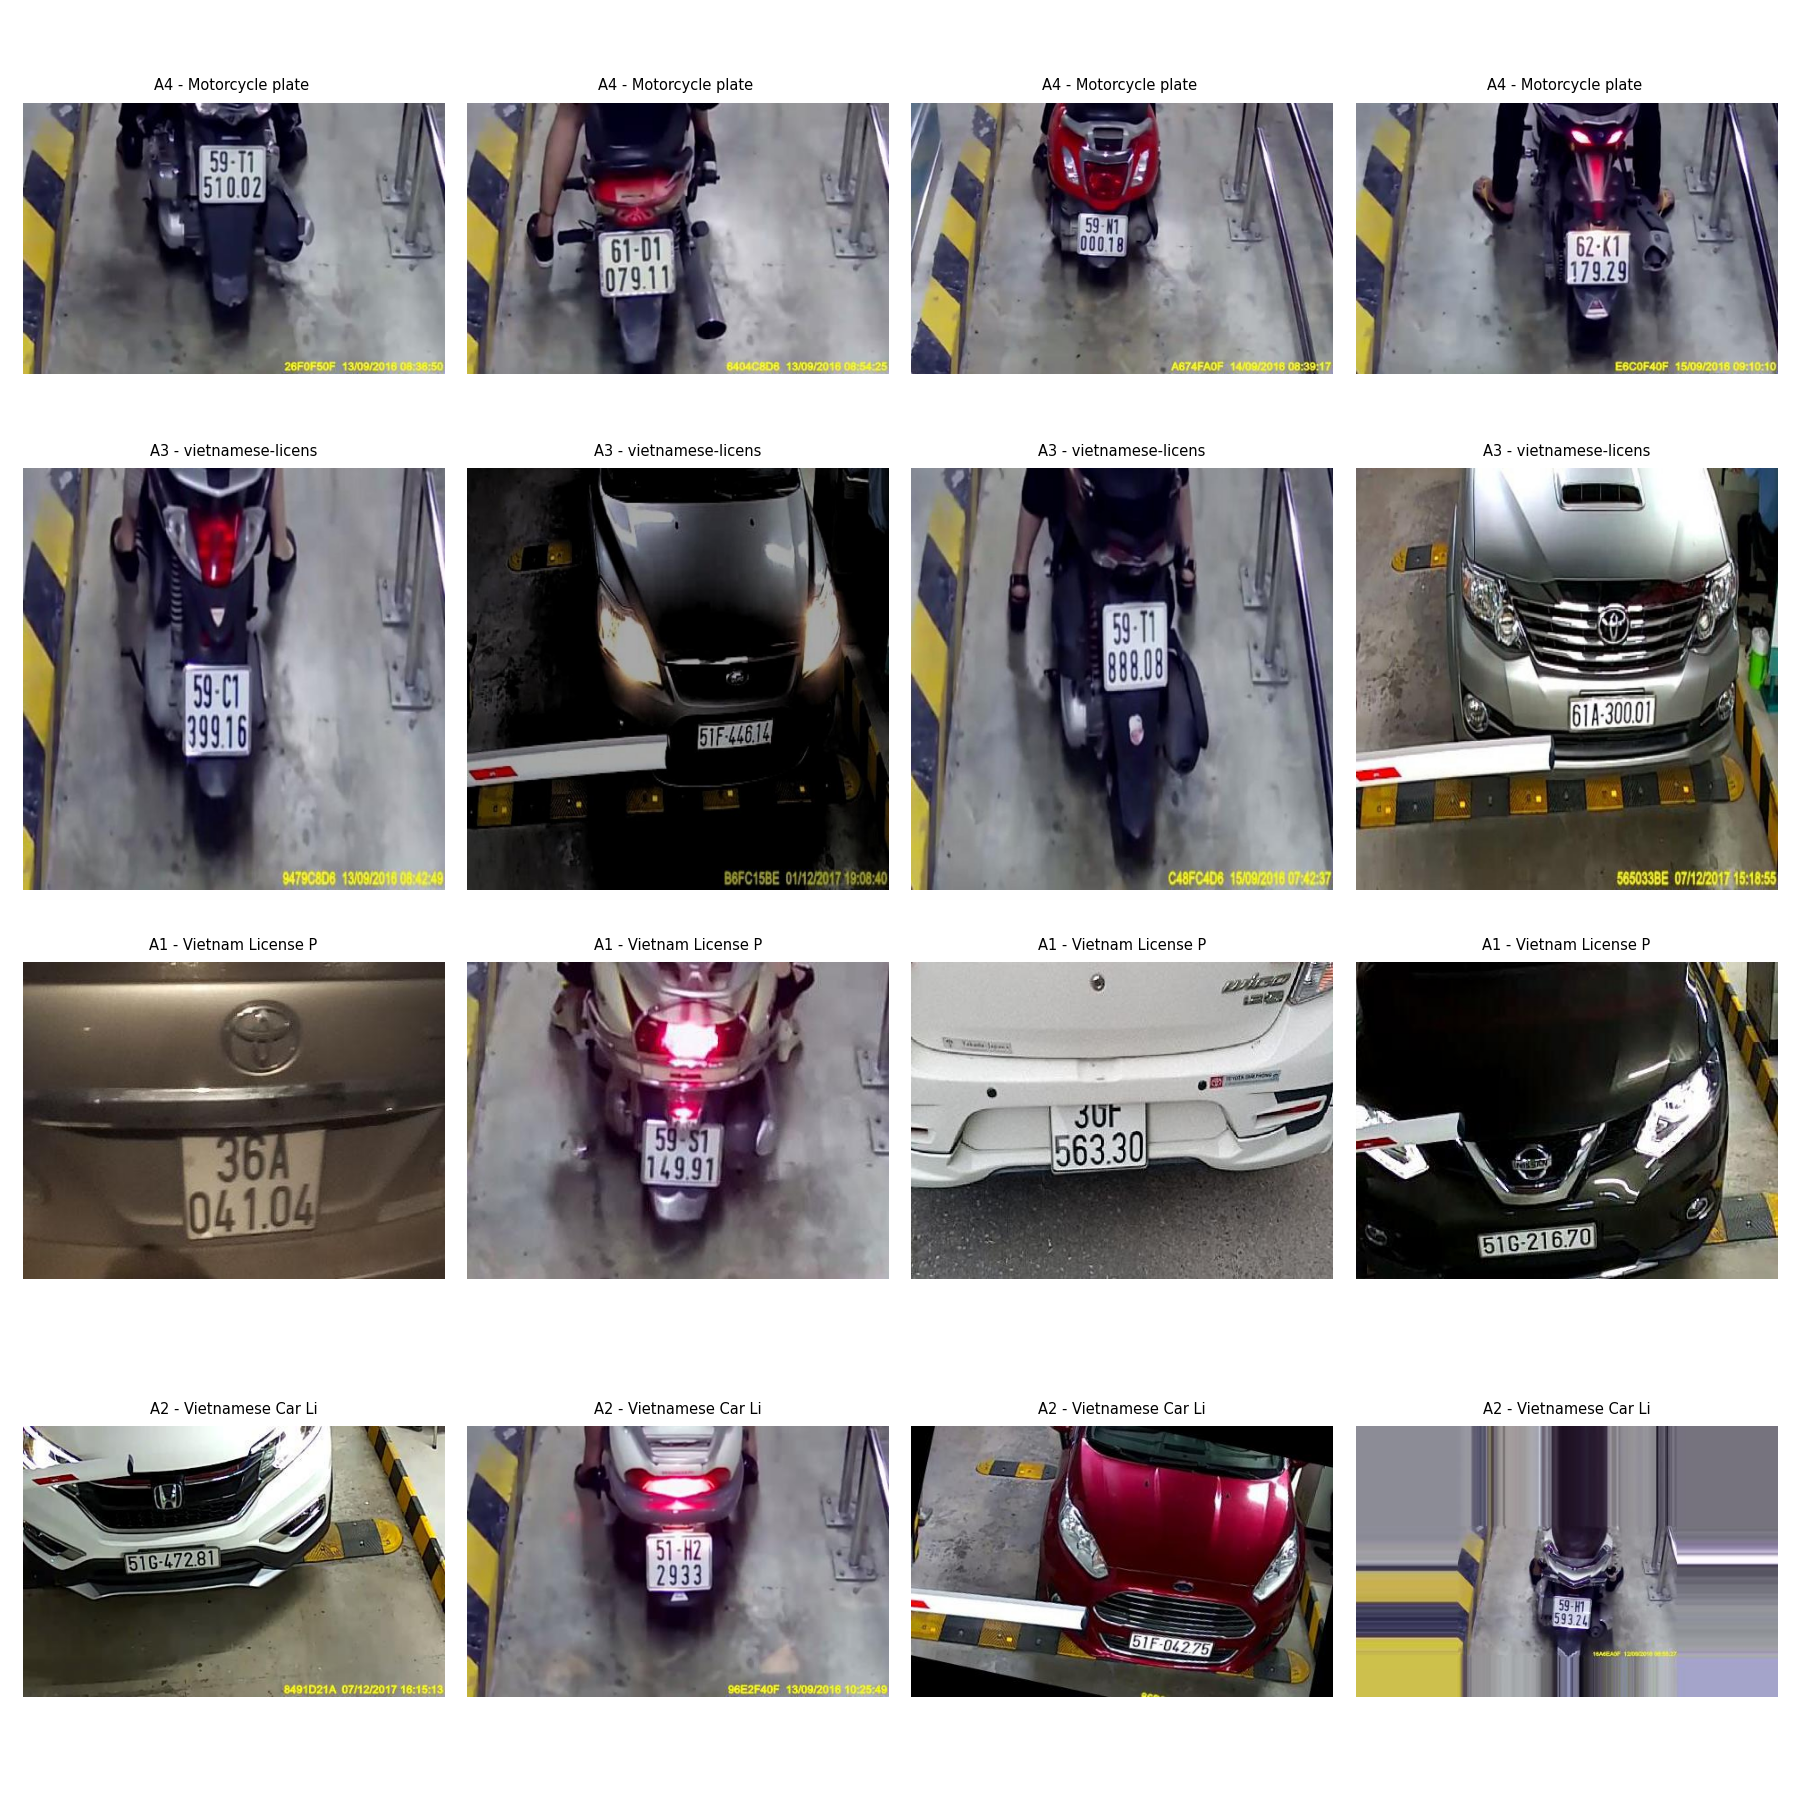
\includegraphics[width=0.90\textwidth]{eda_sample_context.png}
\caption{Ảnh mẫu ngẫu nhiên từ ba bộ dữ liệu, minh họa bối cảnh camera cổng bãi xe.}

\label{fig:eda-sample}
\end{figure}

% =====================================================================
\section{Bộ Dữ Liệu Bổ Sung cho OCR, Màu Biển và Phân Loại Xe}
\label{sec:datasetocrcolor}
% =====================================================================

\subsection{Bộ Dữ Liệu Phát Hiện Biển và OCR}

Bảng~\ref{tab:dataset-ocr} liệt kê các bộ đã tải thực tế phục vụ phát hiện biển, OCR và ký
tự đơn lẻ.

\begin{table}[htbp]
\centering
\caption{Các bộ dữ liệu phát hiện biển, OCR và ký tự đơn lẻ đã tải thực tế.}

{\footnotesize Nguồn: Kaggle \autocite{tanhphp2026vnplatedet,bomaich2022vnplateyolov7,topkek2024vnplateocr,dtkngan2024motorbikeocr,kaggle2022vncharplate}.}
\label{tab:dataset-ocr}
\small
\begin{tabular}{p{3.4cm} p{3.0cm} p{2.0cm} p{3.0cm}}
\toprule
\textbf{Bộ dữ liệu} & \textbf{Số ảnh (thật)} & \textbf{Định dạng} & \textbf{Ghi chú} \\
\midrule
plate\_tanhphp~\autocite{tanhphp2026vnplatedet} & 2.255 (2.998 box) & YOLO bbox, nc=1 & Dùng làm nguồn detect chính bổ sung \\
plate\_bomaich\_yolov7~\autocite{bomaich2022vnplateyolov7} & 498 (780 box) & YOLO bbox, split sẵn & Ảnh cảnh đầy đủ, dùng bổ sung \\
plate\_ocr\_topkek~\autocite{topkek2024vnplateocr} & 12.190 (6.643 crop thật cộng 5.547 sinh tổng hợp) & Crop cộng CSV Name/Label/Type & Nguồn OCR chính; cần tách riêng phần sinh tổng hợp khi đánh giá để không thổi phồng accuracy \\
motorbike\_ocr\_100~\autocite{dtkngan2024motorbikeocr} & 116 & Ảnh cộng chuỗi biển & Tập test cho biển xe máy 2 hàng, chỉ có ảnh ban ngày \\
char\_nguyenquanglinh~\autocite{kaggle2022vncharplate} & 1.839 & Thư mục theo lớp, ảnh 28$\times$28 & Lệch lớp nặng giữa các ký tự; cần augment mạnh cho ký tự hiếm \\
\bottomrule
\end{tabular}
\end{table}

Các kho này không kèm file LICENSE rõ ràng nên đề tài chỉ dùng nội bộ, không phát hành
lại.

\subsection{Phân Tích Màu Biển Số (HSV)}
\label{sec:hsv}

Để phục vụ mô đun phân loại màu biển (Chương~\ref{ch:ocr}), đề tài chạy phân tích HSV trên
599 crop biển thật (từ bộ topkek\_plate\_ocr), tách vùng nền sáng khỏi vùng chữ tối.
Kết quả ở Bảng~\ref{tab:hsv-color}.

\begin{table}[htbp]
\centering
\caption{Phân bố màu nền trên 599 crop biển số thực tế.}

{\footnotesize Phân tích HSV trên crop từ bộ topkek\_plate\_ocr~\autocite{topkek2024vnplateocr}.}
\label{tab:hsv-color}
\begin{tabular}{lrrp{4.5cm}}
\toprule
\textbf{Màu nền} & \textbf{Số crop} & \textbf{Tỷ lệ} & \textbf{Ý nghĩa biển số VN} \\
\midrule
Trắng & 372 & 62,1\% & Xe cá nhân \\
Vàng & 115 & 19,2\% & Xe kinh doanh/dịch vụ \\
Xanh dương & 57 & 9,5\% & Cơ quan nhà nước \\
Đỏ & 37 & 6,2\% & Quân đội \\
\bottomrule
\end{tabular}
\end{table}

Bốn màu tách thành các cụm hue và saturation riêng biệt, cho thấy dùng HSV kết hợp CLAHE
mà không cần CNN riêng cho màu là khả thi. Dữ liệu lệch nặng về màu trắng (62,1\%), phản
ánh tỷ lệ thực của bãi xe dân sự.

\subsection{Bộ Dữ Liệu Phân Loại Xe}

Mô đun phân loại xe (Chương~\ref{ch:phanloai}) dùng A1 cho bước loại xe (ô tô, xe máy, xe
tải) và B5~\autocite{researchprojects2022vehiclebodystyle} cho bước kiểu dáng xe con.

% =====================================================================
\section{Trùng Lặp Gần giữa Tập Huấn Luyện và Tập Kiểm Tra}
\label{sec:dedup}
% =====================================================================

Trước khi đánh giá detector, đề tài so khớp average hash giữa tập huấn luyện và tập kiểm tra
của A1: 230 trong 572 ảnh kiểm tra (khoảng 40\%) có ảnh huấn luyện gần trùng với khoảng cách
Hamming không quá 5. Nguyên nhân là A1 trích từ luồng video liên tục nên các khung kế tiếp
chỉ khác vài pixel; chia ngẫu nhiên theo khung khiến tập kiểm tra rò rỉ từ tập huấn luyện
(data leakage) và thổi phồng chỉ số.

Đề tài loại các ảnh này trước khi đánh giá chính thức, tác động lên mAP trình bày ở
Bảng~\ref{tab:det-dedup}. Với dữ liệu trích từ video, nên chia tập theo thời gian thay vì
ngẫu nhiên theo khung.
         % Chương 3: Dữ liệu
% =====================================================================
%  CHƯƠNG 4 — PHÁT HIỆN XE VÀ BIỂN SỐ          | Phụ trách: Nhật
%  Ngân sách: mục tiêu 5 trang.
%  Nguồn số nội bộ (không in ra báo cáo):
%    experiments.csv (test split, 2026-08-13); results.csv 6 run 50 epoch;
%    a1_dedup_eval.csv (2026-09-12); phash_report.txt (230 cặp Hamming<=5).
% =====================================================================
\chapter{Phát Hiện Xe và Biển Số}
\label{ch:phathien}

Chương này so sánh YOLOv8n và YOLO26n cho phát hiện biển số trên bộ A1, đánh giá trên cả
tập kiểm tra gốc lẫn tập đã khử trùng lặp gần.

\section{Kiến Trúc Mô Hình}
\label{sec:phathien-kientruc}

Kiến trúc hai mô hình đã trình bày ở Mục~\ref{sec:yolov8} và Mục~\ref{sec:yolo26}. Điểm
liên quan trực tiếp đến bài toán là YOLOv8n gán nhãn dương bằng Task-Aligned
Assigner~\autocite{jocher2023yolov8,feng2021tood}, còn YOLO26n bỏ NMS, bỏ DFL và dùng STAL ưu
tiên vật thể nhỏ~\autocite{jocher2026yolo26,chakrabarty2026yolo26nmsfree}, phù hợp với biển số
vốn nhỏ so với khung ảnh~\autocite{zhu2025licenseplate}. Cả hai dùng biến thể nano để vừa
ngân sách độ trễ trên Raspberry Pi 5 (Mục~\ref{sec:pi5bench}).

\section{Thiết Lập Huấn Luyện}
\label{sec:phathien-huanluyen}

Đề tài huấn luyện trên A1 (4.578 ảnh, 5.200 đối tượng biển số) với hai lớp là biển một hàng
(đặc trưng ô tô) và biển hai hàng (đặc trưng xe máy), chia 3.433 ảnh huấn luyện, 573 kiểm
định, 572 kiểm tra. Bảng~\ref{tab:det-hyperparam} liệt kê các siêu tham số chính; mô hình
khởi tạo từ trọng số pretrained COCO, mỗi kiến trúc huấn luyện với ba seed (0, 1, 2) để đánh
giá tính ổn định. Chi tiết augmentation ở Phụ lục~\ref{app:huanluyen}.

\begin{table}[htbp]
\centering
\caption{Siêu tham số huấn luyện detector biển số.}

\label{tab:det-hyperparam}
\begin{tabular}{ll}
\toprule
\textbf{Tham số} & \textbf{Giá trị} \\
\midrule
Kích thước ảnh đầu vào & 640 \\
Số epoch & 50 \\
Batch size & 16 \\
Patience (early stopping) & 10 \\
Optimizer & SGD (mặc định Ultralytics) \\
Learning rate khởi đầu & 0,01 \\
Learning rate cuối & 0,0001 \\
Momentum & 0,937 \\
Weight decay & 0,0005 \\
Warmup epochs & 3 \\
\bottomrule
\end{tabular}
\end{table}

\section{Độ Đo Đánh Giá}
\label{sec:phathien-dodo}

Precision $P = TP/(TP+FP)$ đo tỉ lệ dự đoán đúng trong các dự đoán dương; Recall
$R = TP/(TP+FN)$ đo tỉ lệ biển thật được phát hiện. \textbf{mAP@0,5} là diện tích dưới đường cong Precision-Recall tại ngưỡng IoU = 0,5,
trung bình trên các lớp.
\textbf{mAP@0,5:0,95} lấy trung bình mAP tại các ngưỡng IoU từ 0,5 đến 0,95 bước 0,05, phạt
nặng hơn các bounding box lỏng lẻo nên phản ánh chất lượng định vị chặt hơn. Giá trị mỗi
epoch tính trên tập kiểm định; kết quả cuối cùng báo cáo trên tập kiểm tra.

\section{Kết Quả Phát Hiện}
\label{sec:phathien-ketqua}

\subsection{So Sánh Hai Mô Hình trên Ba Seed}

\begin{table}[htbp]
\centering
\caption{Kết quả phát hiện biển số trên tập kiểm định (epoch 50) theo từng seed.}

\label{tab:det-results}
\begin{tabular}{llcccc}
\toprule
\textbf{Mô hình} & \textbf{Seed} & \textbf{P} & \textbf{R} & \textbf{mAP@0,5} & \textbf{mAP@0,5:0,95} \\
\midrule
\multirow{4}{*}{YOLOv8n} & 0   & 0,988 & 0,987 & 0,994 & 0,867 \\
                          & 1   & 0,990 & 0,992 & 0,994 & 0,873 \\
                          & 2   & 0,986 & 0,991 & 0,994 & 0,866 \\
                          & \textit{Trung bình} & \textit{0,988} & \textit{0,990} & \textit{0,994} & \textit{0,869} \\
\midrule
\multirow{4}{*}{YOLO26n}  & 0   & 0,982 & 0,969 & 0,993 & 0,879 \\
                           & 1   & 0,974 & 0,977 & 0,992 & 0,880 \\
                           & 2   & 0,969 & 0,988 & 0,993 & 0,884 \\
                           & \textit{Trung bình} & \textit{0,975} & \textit{0,978} & \textit{0,993} & \textit{0,881} \\
\bottomrule
\end{tabular}
\end{table}

Bảng~\ref{tab:det-results} cho thấy cả hai mô hình đạt mAP@0,5 trên 0,99 sau 50 epoch.
YOLOv8n có Precision cao hơn (0,988 so với 0,975), còn YOLO26n có mAP@0,5:0,95 cao hơn nhẹ
(0,881 so với 0,869); chênh lệch mAP@0,5 giữa hai mô hình dưới 0,002, nằm trong nhiễu thống
kê của ba seed. Đường cong huấn luyện theo epoch ở Hình~\ref{fig:det-curves}, hội tụ tốt từ
epoch 10 đến 15 với độ lệch chuẩn mAP@0,5 dưới 0,001 giữa các seed.

\begin{figure}[htbp]
\centering
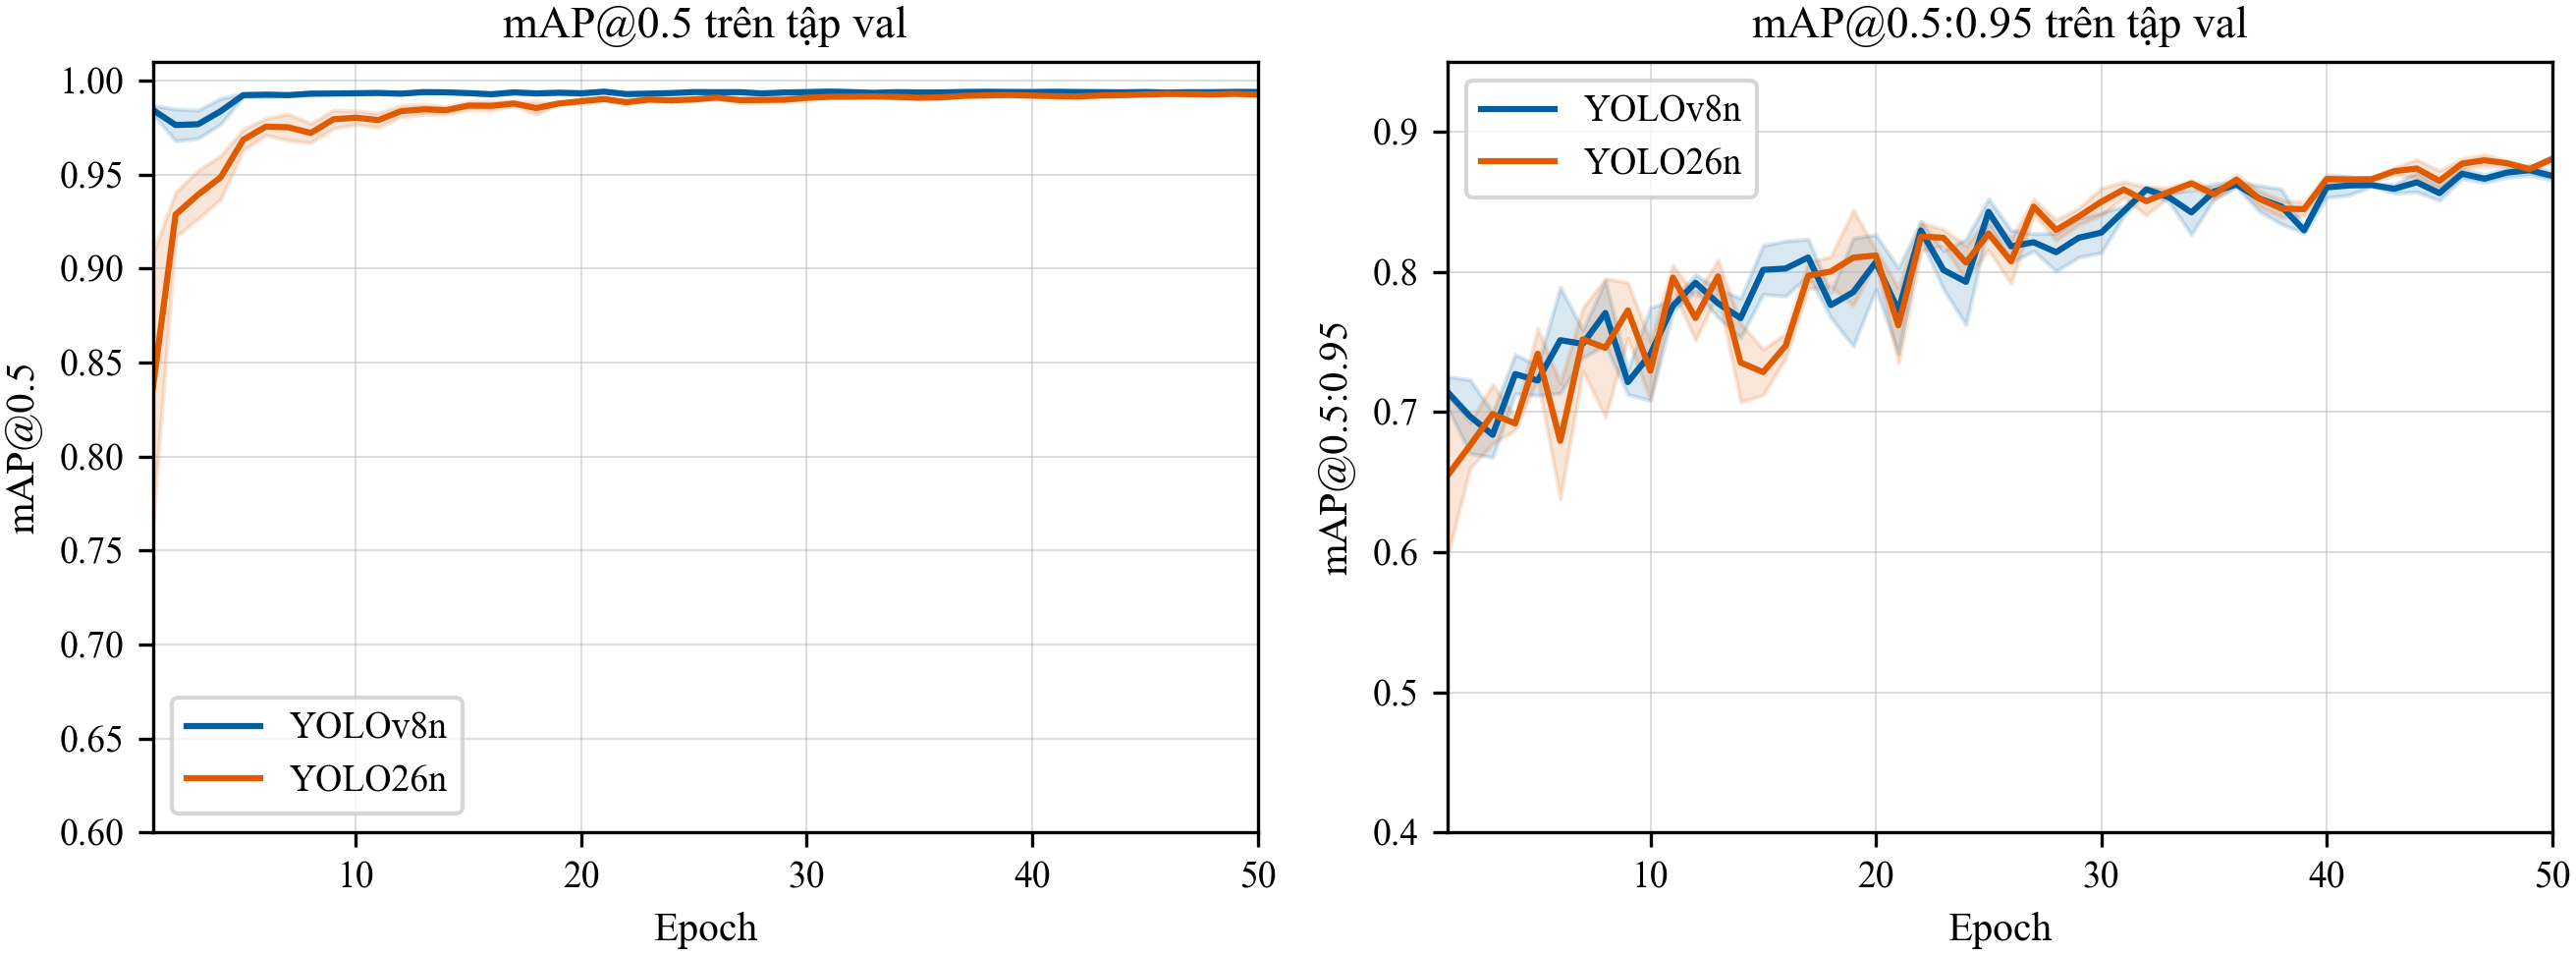
\includegraphics[width=0.92\textwidth]{plate_det_curves.png}
\caption{Đường cong mAP theo epoch trên tập kiểm định, trung bình của ba seed (vùng bóng: độ lệch chuẩn). Trái: mAP@0,5; Phải: mAP@0,5:0,95.}

\label{fig:det-curves}
\end{figure}

Trên tập kiểm tra, YOLOv8n đạt mAP@0,5 = 0,989, mAP@0,5:0,95 = 0,864,
P = 0,990, R = 0,982; YOLO26n đạt mAP@0,5 = 0,980, mAP@0,5:0,95 = 0,859.

\subsection{Đánh Giá Sau Khử Trùng Lặp Gần}

Do khoảng 40\% ảnh kiểm tra của A1 có ảnh huấn luyện gần trùng (Mục~\ref{sec:dedup}),
YOLOv8n (seed 0) được đánh giá lại sau khi loại 230 ảnh này (Bảng~\ref{tab:det-dedup}).

\begin{table}[htbp]
\centering
\caption{Hiệu năng YOLOv8n (seed 0) trên tập kiểm tra trước và sau khi khử trùng lặp gần (Hamming $\leq 5$).}
\label{tab:det-dedup}
\begin{tabular}{lcccccc}
\toprule
\textbf{Tập kiểm tra} & \textbf{Số ảnh} & \textbf{P} & \textbf{R} & \textbf{mAP@0,5} & \textbf{mAP@0,5:0,95} \\
\midrule
Gốc (có near-dup) & 572 & 0,989 & 0,986 & 0,989 & 0,864 \\
Đã khử trùng lặp  & 342 & 0,983 & 0,980 & 0,983 & 0,834 \\
\midrule
\textit{Chênh lệch}  & \textit{$-$230} & \textit{$-$0,006} & \textit{$-$0,006} & \textit{$-$0,006} & \textit{$-$0,030} \\
\bottomrule
\end{tabular}
\end{table}

Sau khi loại ảnh gần trùng, mAP@0,5 chỉ giảm 0,006 (từ 0,989 xuống 0,983) nhưng
mAP@0,5:0,95 giảm 0,030 (từ 0,864 xuống 0,834): mô hình đã ghi nhớ vị trí biển trong các khung
gần trùng nên đạt IoU cao khi gặp lại. Vì vậy mAP@0,5 bằng 0,983 là ước lượng bảo thủ và đáng
tin hơn cho dữ liệu chưa thấy.

\section{Thảo Luận}
\label{sec:phathien-thaoluan}

YOLO26n nhỉnh hơn ở mAP@0,5:0,95, gợi ý việc bỏ DFL và dùng STAL cải thiện định vị; YOLOv8n
có Precision cao hơn, tức ít báo nhầm, có lợi ở bãi xe vì một phát hiện nhầm dẫn tới lỗi tra
biển. YOLOv8n chỉ khoảng 3,2 triệu tham số và 8,7 GFLOPs~\autocite{jocher2023yolov8}.

Đề tài chọn YOLOv8n (seed 0) cho pipeline vì hệ sinh thái xuất ONNX trên CPU ARM trưởng thành
hơn và Precision cao hơn, trong khi mAP@0,5 của hai mô hình tương đương. YOLO26n là ứng viên
nâng cấp khi tối ưu thiết bị biên (Mục~\ref{sec:huongphattrien}).
       % Chương 4: Phát hiện xe và biển số
% =====================================================================
%  CHƯƠNG 5. NHẬN DẠNG KÝ TỰ VÀ MÀU NỀN BIỂN SỐ   | Nhật (OCR) + Đức (màu)
%  Ngân sách: mục tiêu 7 trang. Viết high-level, không nhắc mã nguồn/hàm/đường dẫn.
%  Nguồn số nội bộ (không in): ocr_full_progression.csv, ocr_comparison.csv,
%    ocr_vnplate_results.csv (a1/vn_plate), topkek 37 ký tự.
% =====================================================================
\chapter{Nhận Dạng Ký Tự và Màu Nền Biển Số}
\label{ch:ocr}

% =====================================================================
\section{Dữ Liệu OCR}
\label{sec:ocr-dulieu}
% =====================================================================

\subsection{Dữ Liệu Huấn Luyện}

Nguồn chính là bộ topkek\_plate\_ocr~\autocite{topkek2024vnplateocr}, gồm 6.643 crop biển thật
và 5.547 crop sinh tổng hợp. Bố cục
biển được suy từ tỉ lệ khung ảnh (rộng trên cao nhỏ hơn 2,0 coi là biển hai dòng). Tập chia
80/10/10 phân tầng theo bố cục, giữ crop sinh tổng hợp riêng và chỉ dùng khi huấn luyện
(Bảng~\ref{tab:ocr-split}, phân bố ở Hình~\ref{fig:ocr-data-dist}).

\begin{table}[htbp]
\centering
\caption{Phân chia tập dữ liệu OCR theo split và bố cục biển.}

{\footnotesize Nguồn: bộ topkek\_plate\_ocr~\autocite{topkek2024vnplateocr}, chia phân tầng theo tỉ lệ bố cục.}
\label{tab:ocr-split}
\begin{tabular}{lrrr}
\toprule
Split & Biển 1 dòng & Biển 2 dòng & Tổng \\
\midrule
train & 1.496 & 3.817 & 5.313 \\
val   & 187   & 477   & 664   \\
test  & 188   & 478   & 666   \\
Sinh tổng hợp (chỉ train) & \multicolumn{2}{c}{(không tách theo bố cục)} & 5.547 \\
\bottomrule
\end{tabular}
\end{table}

\begin{figure}[htbp]
\centering
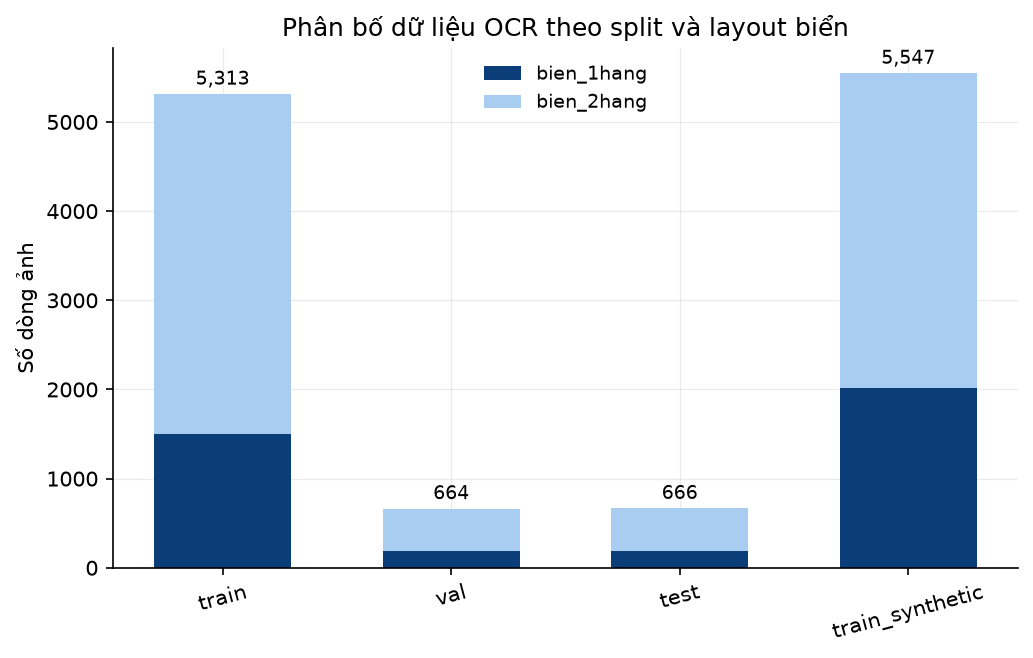
\includegraphics[width=0.85\textwidth]{plate_ocr_data_distribution.png}
\caption{Phân bố dữ liệu OCR theo split và bố cục biển.}

\label{fig:ocr-data-dist}
\end{figure}

\subsection{Tập Test Độc Lập}

Tập test của topkek cùng nguồn gốc với tập huấn luyện nên chưa đủ đánh giá tổng quát hoá. Đề
tài xây thêm tập test độc lập từ bộ vn\_plate (Roboflow, CC BY 4.0, 1.005 ảnh) có sẵn bounding
box nhưng không có nhãn chuỗi: cắt biển theo bounding box, chọn ngẫu nhiên 100 biển rồi gán
nhãn thủ công mà không nhìn dự đoán của mô hình, giữ lại 96 biển đọc được (45 biển một dòng,
51 biển hai dòng). Tập này có độ phân giải sát điều kiện triển khai hơn: trung vị 52 px mỗi
dòng ký tự, so với 19 px ở topkek.

% =====================================================================
\section{Kiến Trúc}
\label{sec:ocr-kientruc}
% =====================================================================

Đề tài so sánh mô hình tự huấn luyện với hai engine OCR pretrained làm mốc: RapidOCR (dòng
PP-OCRv3, chạy qua ONNX Runtime)~\autocite{rapidocr} và EasyOCR (CRNN pretrained, bảng ký tự
tiếng Anh)~\autocite{easyocr}. Mô hình riêng là một CRNN gồm phần trích đặc trưng tích chập,
một lớp BiLSTM và đầu ra CTC, ảnh vào ảnh xám 48$\times$128 pixel, tổng khoảng 425 nghìn tham
số, nhỏ nhờ bảng ký tự thu hẹp đúng cấu trúc biển Việt Nam; kiến trúc theo Shi và cộng sự
cùng Graves và cộng sự~\autocite{shi2017crnn,graves2006ctc}. Cả ba dùng chung luồng xử lý:
chỉnh hình học, tách dòng nếu là biển hai dòng, đọc từng dòng, ghép chuỗi và chuẩn hoá theo
quy tắc biển Việt Nam.

\subsection{Nắn Phối Cảnh Thay Cho Xoay Phẳng}

Xoay biển trong mặt phẳng ảnh không xử lý được biến dạng phối cảnh khi camera gắn cao và lệch
bên. Đề tài nắn 4 góc biển, lấy từ đầu ra phân vùng của mô hình phát hiện, về hình chữ nhật
bằng phép biến đổi phối cảnh, tăng tỉ lệ đọc đúng trên A1 từ 44\% lên 76\%
(Bảng~\ref{tab:ocr-perspective}).

\begin{table}[htbp]
\centering
\caption{So sánh hai cách xử lý hình học trên tập A1 (ảnh cổng bãi xe thật).}

{\footnotesize Đếm thủ công trên các biển đọc được bằng mắt trong tập A1.}
\label{tab:ocr-perspective}
\begin{tabular}{lr}
\toprule
Cách xử lý hình học & Đọc đúng \\
\midrule
Xoay phẳng & 8/18 (44\%) \\
\textbf{Nắn phối cảnh 4 điểm} & \textbf{13/17 (76\%)} \\
\bottomrule
\end{tabular}
\end{table}

% =====================================================================
\section{Huấn Luyện và Xử Lý Dữ Liệu}
\label{sec:ocr-caitien}
% =====================================================================

Mỗi mẫu huấn luyện là một dòng ký tự; biển hai dòng được tách thành hai mẫu. Bảng ký tự ban
đầu gồm 36 ký tự (0 đến 9, A đến Z), mở rộng thêm ``Đ'' ở Mục~\ref{sec:ocr-charset37}; siêu
tham số chi tiết ở Bảng~\ref{tab:app-ocr}.

\subsection{Xử Lý Dữ Liệu Sinh Tổng Hợp}

Ảnh sinh tổng hợp chiếm khoảng một nửa dữ liệu huấn luyện nhưng là biển render sắc nét, không
nhiễu, không nghiêng, trung vị 45 đến 50 px mỗi dòng so với 19 px của crop thật. Đề tài so
sánh ba cách dùng ảnh này, các yếu tố khác giữ nguyên: giữ nguyên, bỏ hẳn, và hạ cấp cho khớp
phân phối ảnh thật (thu nhỏ theo phân phối px/dòng thực nghiệm rồi thêm nhiễu và nén). Cách
hạ cấp tốt nhất trên cả hai tập test, bỏ hẳn là kém nhất (Bảng~\ref{tab:ocr-v0v2}); lọc bỏ
crop dưới 25 px/dòng cũng cho kết quả kém hơn. Số lượng dữ liệu vì vậy quan trọng hơn độ đồng
nhất phân phối.

\begin{table}[htbp]
\centering
\caption{Accuracy theo cách xử lý dữ liệu sinh tổng hợp (bảng 36 ký tự).}

\label{tab:ocr-v0v2}
\begin{tabular}{lrr}
\toprule
Cách xử lý & topkek test & vn\_plate test \\
\midrule
Giữ nguyên & 51,1\% & 62,5\% \\
Bỏ hẳn ảnh sinh tổng hợp & 49,5\% & 51,0\% \\
\textbf{Hạ cấp khớp phân phối} & \textbf{54,2\%} & \textbf{64,6\%} \\
\bottomrule
\end{tabular}
\end{table}

\subsection{Ranh Giới Nhãn Biển Hai Dòng}

Nhãn biển hai dòng là một chuỗi ghép không chỉ rõ ranh giới dòng; tách sai khiến mô hình học
bỏ ký tự cuối dòng trên. Tách nhãn theo dấu cách trong nhãn gốc sửa được khoảng 10,6\% nhãn
biển hai dòng bị tách sai và gần như xoá chênh lệch giữa biển một dòng và hai dòng.

\subsection{Kiểm Soát Nhiễu Ngẫu Nhiên Giữa Các Lần Huấn Luyện}

Hai lần huấn luyện cùng cấu hình (bảng 36 ký tự, sau khi sửa nhãn hai dòng), chỉ khác seed 42
và 123, cho accuracy trên vn\_plate 87,5\% và 92,7\%, lệch 5,2 điểm phần trăm. Với tập test
nhỏ, mức lệch này đủ làm sai kết luận rút ra từ một lần huấn luyện, nên đề tài cố định seed và
chọn mô hình theo CER trên tập kiểm định thay vì theo điểm cao nhất trên tập test. Hình~\ref{fig:ocr-loss-curves} trình bày đường mất mát và
CER kiểm định theo epoch.

\begin{figure}[htbp]
\centering

\includegraphics[width=0.90\textwidth]{plate_ocr_progression.png}
\caption{Đường mất mát huấn luyện và CER/accuracy kiểm định theo epoch.}

\label{fig:ocr-loss-curves}
\end{figure}

% =====================================================================
\section{Mở Rộng Bảng Ký Tự Lên 37 Ký Tự và Model Triển Khai}
\label{sec:ocr-charset37}
% =====================================================================

Để đọc seri MĐ và TĐ của xe máy điện, đề tài mở bảng ký tự lên 37 ký tự và giữ ``Đ'' trong
toàn bộ khâu chuẩn hoá nhãn và hậu xử lý, vốn từng vô tình loại bỏ ký tự này. Mô hình triển
khai được đo trên ba tập test có độ phân giải tăng dần (Bảng~\ref{tab:ocr-deployed}).

\begin{table}[htbp]
\centering
\caption{Kết quả model triển khai CRNN 37 ký tự trên ba tập test (accuracy mức cả biển).}

\label{tab:ocr-deployed}
\begin{tabular}{lrrr}
\toprule
& topkek (n = 666) & vn\_plate (n = 96) & a1 (n = 172) \\
\midrule
Accuracy toàn biển & 56,6\% & 80,2\% & 91,9\% \\
Biển 1 dòng & 59,6\% & 75,6\% & 91,5\% \\
Biển 2 dòng & 55,4\% & 84,3\% & 92,3\% \\
CER & 0,183 & 0,031 & 0,015 \\
\bottomrule
\end{tabular}
\end{table}

Tập a1 (172 crop cắt từ ảnh camera cổng, đã nắn phối cảnh) gần nhất với điều kiện chạy thật;
trên tập này mô hình đạt \textbf{91,9\%} accuracy mức cả biển (khoảng tin cậy Wilson 95\% từ
86,8\% đến 95,1\%) với CER 0,015, nên là con số dùng để đối chiếu tiêu chí đọc biển trên
90\% của đề cương. Trên cả ba tập, biển hai dòng không kém biển một
dòng quá 4,2 điểm phần trăm, cho thấy bước tách dòng xử lý tốt cả hai bố cục.

Đóng góp của ký tự ``Đ'' là mở rộng độ phủ chứ không phải tăng accuracy tổng thể: trên 17
biển có ``Đ'' trong tập test, mô hình 37 ký tự đọc đúng ``Đ'' ở 11/17 biển (khớp toàn chuỗi
ở 8/17), trong khi mô hình 36 ký tự cũ không đọc được biển nào (0/17). Bản ONNX cho dự đoán
trùng khớp bản huấn luyện trên toàn bộ 666 biển kiểm tra.

% =====================================================================
\section{Kết Quả So Sánh và Phân Tích Độ Phân Giải}
\label{sec:ocr-ketqua}
% =====================================================================

\subsection{So Sánh Với Hai Engine Pretrained}

Trên tập test topkek (666 crop thật), mô hình CRNN riêng vượt cả hai baseline trên mọi tiêu
chí cùng lúc (Bảng~\ref{tab:ocr-compare}): chính xác hơn nhiều lần, nhỏ hơn RapidOCR khoảng 6
lần và EasyOCR khoảng 58 lần, và nhanh hơn cả hai trên CPU. Nguyên nhân là phạm vi bài toán:
hai mô hình pretrained mang bảng ký tự tổng quát, còn CRNN riêng chỉ cần phân biệt bộ ký tự
cố định theo cấu trúc biển Việt Nam (Hình~\ref{fig:ocr-compare}).

\begin{table}[htbp]
\centering
\caption{So sánh ba phương pháp OCR trên tập test topkek (666 biển thật).}

{\footnotesize CRNN riêng đo ở bảng 36 ký tự, trước bước mở rộng ``Đ''; kích thước tính cả mô hình phát hiện văn bản của EasyOCR; thời gian đo trên CPU máy huấn luyện, cho một lần đọc.}
\label{tab:ocr-compare}
\begin{tabular}{lrrrr}
\toprule
Phương pháp & Accuracy & CER & Kích thước & CPU inference \\
\midrule
RapidOCR~\autocite{rapidocr} & 34,2\% & 34,2\% & 10,7 MB & 7,20 ms \\
EasyOCR~\autocite{easyocr}   & 11,7\% & 51,9\% & 98,3 MB & 16,65 ms \\
\textbf{CRNN riêng}         & \textbf{58,9\%} & \textbf{17,4\%} & \textbf{1,7 MB} & \textbf{1,69 ms} \\
\bottomrule
\end{tabular}
\end{table}

\begin{figure}[htbp]
\centering
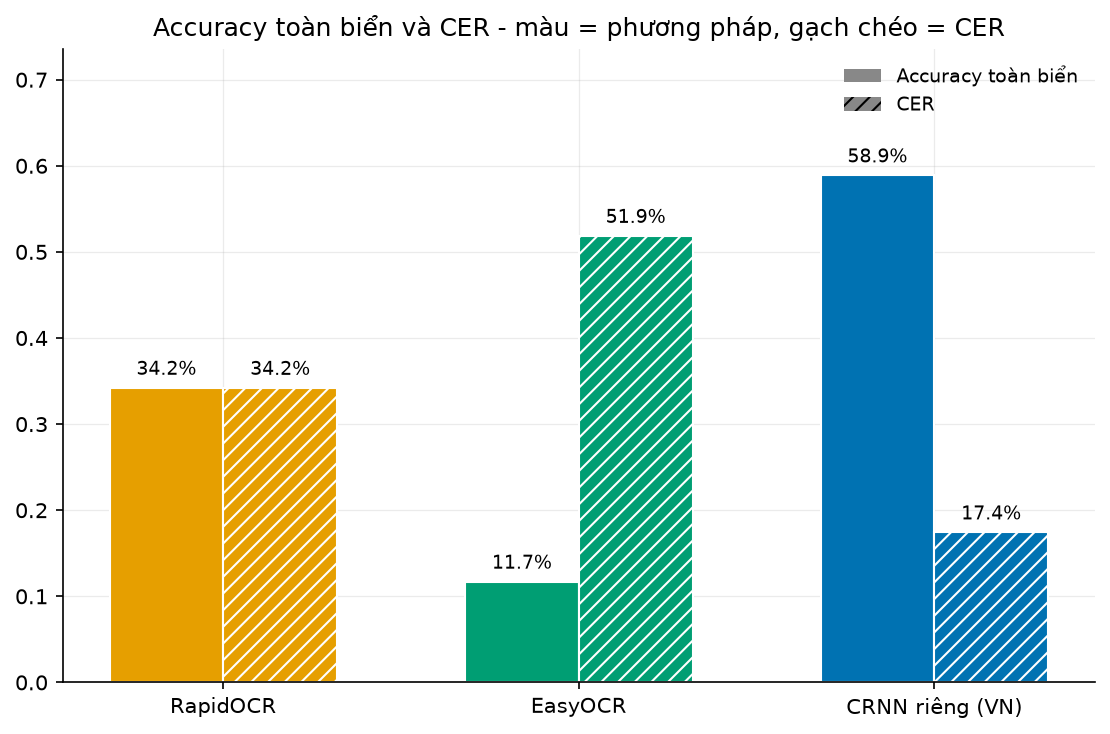
\includegraphics[width=0.82\textwidth]{plate_ocr_accuracy_comparison.png}
\caption{Accuracy toàn biển và CER của ba phương pháp trên tập test topkek.}

\label{fig:ocr-compare}
\end{figure}

\subsection{Phân Tích Theo Dải Độ Phân Giải}

Cùng một mô hình cho hai con số cách nhau 24 điểm phần trăm trên hai tập test (56,6\% so với
80,2\%). Tách theo dải độ phân giải (Bảng~\ref{tab:ocr-resolution-band}) cho thấy nguyên nhân
là tỉ lệ ảnh khó giữa hai tập rất khác nhau, không phải mô hình thiếu ổn định: ở dải đủ nét
(từ 40 px/dòng trở lên) mô hình đạt 93,9\% trên topkek, vượt mục tiêu 90\%, nhưng dải đó chỉ
chiếm 7,4\% tập topkek trong khi hơn nửa tập dưới 20 px, gần như không đọc được bằng mắt. Tập
vn\_plate có phân bố ngược (87,5\% ảnh từ 40 px trở lên) nên trung bình cao hơn dù dùng chung
mô hình. Vì vậy accuracy toàn tập chỉ có ý nghĩa khi đọc kèm phân bố độ phân giải. Một số mẫu dự đoán ở Hình~\ref{fig:ocr-samples}.

\begin{table}[htbp]
\centering
\caption{Accuracy theo dải độ phân giải (bảng 36 ký tự). Tập vn\_plate không có ảnh dưới 20 px/dòng.}

\label{tab:ocr-resolution-band}
\begin{tabular}{lrrrr}
\toprule
Dải độ phân giải & Tỉ lệ trong topkek & Accuracy (topkek) & Tỉ lệ trong vn\_plate & Accuracy (vn\_plate) \\
\midrule
Dưới 20 px/dòng & 52,3\% & 46,6\% & 0\% & n/a \\
20 đến 30 px    & 25,8\% & 61,6\% & 1,0\% & 100\% \\
30 đến 40 px    & 14,6\% & 80,4\% & 11,5\% & 100\% \\
\textbf{Từ 40 px trở lên} & 7,4\% & \textbf{93,9\%} & 87,5\% & 85,7\% \\
\bottomrule
\end{tabular}
\end{table}

\begin{figure}[htbp]
\centering

\includegraphics[width=0.82\textwidth]{plate_ocr_sample_predictions.png}
\caption{Mẫu dự đoán của mô hình CRNN 37 ký tự trên tập test.}

\label{fig:ocr-samples}
\end{figure}

% =====================================================================
\section{Hậu Xử Lý Theo Quy Định Biển Số Việt Nam}
\label{sec:ocr-hauxy}
% =====================================================================

Sau khi ghép chuỗi, kết quả được chuẩn hoá theo vị trí kỳ vọng: vị trí số quy về chữ số (O
thành 0, I thành 1, B thành 8, S thành 5, Z thành 2), vị trí seri quy về chữ cái, rồi kiểm
tra khớp định dạng. Seri có thể gồm một hoặc hai chữ cái: theo Thông tư
79/2024/TT-BCA~\autocite{tt792024bca} (hiệu lực 01/01/2025), biển xe máy thống nhất seri hai
chữ cái kèm 5 chữ số, biển seri cũ một chữ một số chỉ dùng đến hết 31/12/2025, và biển seri
hai chữ cái đã chiếm 15\% đến 19\% tập topkek. Biểu thức kiểm tra nhận cả hai trường hợp. Với
biển hai dòng, độ dài dòng trên cho biết chỗ ngắt khi hiển thị nên không cần suy đoán; chỉ
biển một dòng mới phải suy đoán theo độ dài phần số.

% =====================================================================
\section{Nhận Diện Màu Nền Biển Số}
\label{sec:mau-bien}
% =====================================================================

\subsection{Vai Trò và Phương Pháp}

Màu nền biển xác định nhóm chủ xe theo pháp luật (Bảng~\ref{tab:maubienso}) và được hệ thống
dùng để phân nhóm xe, áp biểu phí (Chương~\ref{ch:hethong}); phân bố màu trên dữ liệu thật ở
Bảng~\ref{tab:hsv-color}.

Đề tài dùng không gian màu HSV vì kênh Hue và Saturation tách rõ màu sắc khỏi độ sáng, giảm
ảnh hưởng biến thiên ánh sáng: trắng có Saturation thấp; vàng, xanh dương và đỏ nằm ở các dải
Hue riêng biệt. Thuật toán đếm pixel nền thuộc từng cụm màu rồi chọn nhãn chiếm đa số, kèm
điểm tin cậy theo tỉ lệ pixel nền được nhận diện.

\subsection{Khử Nhiễu Viền Bằng Otsu và Phát Hiện Contour}

Crop biển thường chứa viền thừa lẫn màu sơn xe hoặc viền đen, gây nhầm màu (ví dụ một biển
trắng từng bị phân loại thành xanh do pixel ở dải viền). Đề tài bổ sung bước tách vùng nền
trước khi đếm màu: tăng tương phản cục bộ bằng CLAHE, phân tách vùng sáng và tối bằng ngưỡng
Otsu, lấy vùng sáng liền khối lớn nhất làm nền biển rồi cắt động theo vùng đó. Cơ chế an toàn
giữ nguyên crop gốc nếu vùng nền tìm được quá nhỏ (dưới 30\% diện tích), tránh cắt sai.

\subsection{Kết Quả và Giới Hạn 2/4 Màu}

Trên tập nhãn màu hiện có gồm 178 crop hai lớp trắng và đỏ, mô đun phân loại đúng toàn bộ
(178/178), gồm cả biển đỏ chữ sáng trên nền tối vốn từng bị nhầm thành trắng. Tập này chưa có
nhãn màu vàng và xanh nên mới đánh giá định lượng được 2 trong 4 màu; biển vàng dưới đèn
huỳnh quang có nguy cơ bị nhầm thành trắng do saturation giảm.

% =====================================================================
\section{Thảo Luận}
\label{sec:ocr-thao-luan}
% =====================================================================

Độ chính xác OCR chịu tác động của ba yếu tố độc lập, mỗi yếu tố một cách xử lý: chất lượng
ảnh (thêm dữ liệu đúng phân phối, không lọc bớt), góc chụp chéo (nắn phối cảnh) và chất lượng
nhãn (tách đúng ranh giới hai dòng).

Về triển khai, mỗi dòng ký tự cần tối thiểu khoảng 40 px. Con số này phụ thuộc vị trí và góc
camera hơn là số megapixel (ảnh gốc A1 rộng tới 4.032 px nhưng biển chỉ khoảng 31 px/dòng vì
xe ở xa), nên cần đặt camera gần hoặc thu hẹp góc nhìn thay vì mua camera phân giải cao hơn.
Tập vn\_plate chỉ có 96 biển nên số liệu trên tập này nên đọc như xu hướng.
    % Chương 5: Nhận dạng ký tự và màu nền biển số
% =====================================================================
%  CHƯƠNG 6. PHÂN LOẠI PHƯƠNG TIỆN                | Phụ trách: Nhật
%  Viết high-level, không nhắc mã nguồn/hàm/đường dẫn.
%  Model triển khai: loại xe = ResNet18; kiểu dáng = MobileNetV3-Small.
% =====================================================================
\chapter{Phân Loại Phương Tiện}
\label{ch:phanloai}

Module phân loại phương tiện gồm ba bước nối tiếp: (1) \textbf{loại xe} (mô hình tự huấn
luyện, chạy trên cả khung hình, cho nhãn ô tô, xe máy hoặc xe tải); (2) \textbf{định vị xe}
(mô hình YOLO pretrained COCO, không huấn luyện thêm, chỉ tìm và cắt vùng xe cho bước~3);
(3) \textbf{kiểu dáng xe con} (chỉ chạy khi bước~1 ra ô tô và bước~2 cắt được vùng xe; mô
hình tự huấn luyện, ba lớp Sedan, Gầm cao, Xe tải). Bước~1 thay cho việc dùng
thẳng nhãn lớp COCO của YOLO, vốn sai nhiều trên ảnh cận cảnh camera cổng
(Mục~\ref{sec:phanloai-ketqua}).

\textbf{Về phạm vi so với đề cương.} Đề cương yêu cầu bốn lớp (ô tô, xe máy, xe tải, xe
buýt); mô hình hiện phân loại được ba lớp. Lớp xe buýt chưa có mô hình riêng do thiếu ảnh xe
khách đúng góc camera cổng, và nhãn xe buýt của YOLO pretrained bị bỏ vì đo được là sai.

\section{Dữ Liệu}
\label{sec:phanloai-dulieu}

\subsection{Dữ liệu cho bước loại xe}

Nguồn là bộ A1 (cùng dữ liệu module phát hiện biển số), chia theo năm nhóm ảnh với nội dung
khác nhau, đã xem tay xác nhận (Bảng~\ref{tab:vt-sources}).

\begin{table}[htbp]
\centering
\caption{Các nhóm ảnh trong bộ A1 dùng cho bước loại xe.}
\label{tab:vt-sources}

\begin{tabular}{lrp{7.5cm}}
\toprule
\textbf{Nhóm} & \textbf{Số ảnh} & \textbf{Nội dung} \\
\midrule
Ô tô cận cảnh & 989 & Ô tô kiểu camera barrier, thuần một loại \\
Xe máy cận cảnh & 1.747 & Xe máy kiểu CCTV cổng, thuần một loại \\
Ảnh phố hỗn hợp & 925 & Nhiều loại xe, hậu cảnh lộn xộn \\
Cắt cực sát & 917 & Chỉ thấy biển và ca-lăng, không dùng cho phân loại loại xe \\
\bottomrule
\end{tabular}
\end{table}

\textbf{Lần huấn luyện đầu mắc lỗi học tắt (shortcut learning).} Khi mỗi lớp chỉ lấy từ đúng
một nguồn ảnh (ô tô từ ảnh cận cảnh, xe máy từ ảnh cận cảnh, xe tải từ ảnh phố), mô hình đạt
100\% trên tập test riêng nhưng chỉ đúng 1 trên 13 ảnh phố thật ngoài tập train, gần như mọi
ảnh bị đoán thành xe tải, vì đó là lớp duy nhất có ảnh phong cách đường phố. Mô hình đã học
nguồn ảnh và góc camera thay vì hình dáng xe.

Cách khắc phục là trộn phong cách ảnh cho từng lớp, buộc mô hình học hình dáng xe: bổ sung
ảnh phố cho lớp ô tô và xe máy bên cạnh ảnh cận cảnh gốc, và xem tay toàn bộ ứng viên cho lớp
xe tải vì độ tin cậy của detector không đủ để lọc tự động. Tập chia 70/15/15 với seed cố định
(Bảng~\ref{tab:vt-split}); lớp xe tải mỏng hơn nhiều nên mất cân bằng được xử lý bằng trọng
số lớp trong hàm mất mát.

\begin{table}[htbp]
\centering
\caption{Số ảnh theo lớp và split của bước loại xe.}
\label{tab:vt-split}

\begin{tabular}{lrrrr}
\toprule
\textbf{Lớp} & \textbf{Train} & \textbf{Valid} & \textbf{Test} & \textbf{Tổng} \\
\midrule
Ô tô & 309 & 66 & 67 & 442 \\
Xe máy & 335 & 72 & 71 & 478 \\
Xe tải & 51 & 11 & 11 & 73 \\
\midrule
\textbf{Tổng} & 695 & 149 & 149 & 993 \\
\bottomrule
\end{tabular}
\end{table}

\subsection{Dữ liệu cho bước kiểu dáng xe con}

Bộ B5 (Vehicle Body Style Dataset, Roboflow, CC BY 4.0) gồm 10.000 ảnh (train 7.014, valid
1.999, test 987) với 12 kiểu dáng gốc, là nguồn duy nhất cho bước kiểu dáng. Mười hai kiểu
dáng được gộp thành ba nhóm thực dụng cho nhu cầu vận hành bãi xe (Bảng~\ref{tab:b5-mapping}).
Ảnh được cắt theo bounding box gốc với biên 10\%, giữ nguyên split
(Bảng~\ref{tab:b5-split}, Hình~\ref{fig:phanloai-phanboo}).

\begin{table}[htbp]
\centering
\caption{Gộp 12 kiểu dáng gốc B5 thành 3 lớp phân loại.}
\label{tab:b5-mapping}
{\footnotesize Nguồn: bộ B5~\autocite{researchprojects2022vehiclebodystyle}, gộp lớp theo đề tài.}
\begin{tabular}{ll}
\toprule
\textbf{Lớp mới} & \textbf{Kiểu dáng gốc B5 gộp vào} \\
\midrule
Sedan & Sedan, Fastback, Hatchback, Wagon, Convertible, Hardtop Convertible, Sports \\
Gầm cao & SUV, Crossover, MPV, Minibus \\
Xe tải & Pickup Truck \\
\bottomrule
\end{tabular}
\end{table}

\begin{table}[htbp]
\centering
\caption{Số ảnh theo lớp và split sau khi gộp từ B5.}
\label{tab:b5-split}

\begin{tabular}{lrrr}
\toprule
\textbf{Lớp} & \textbf{Train} & \textbf{Valid} & \textbf{Test} \\
\midrule
Sedan & 4.102 & 1.166 & 569 \\
Gầm cao & 2.325 & 670 & 334 \\
Xe tải & 587 & 163 & 84 \\
\midrule
\textbf{Tổng} & 7.014 & 1.999 & 987 \\
\bottomrule
\end{tabular}
\end{table}

\begin{figure}[htbp]
\centering
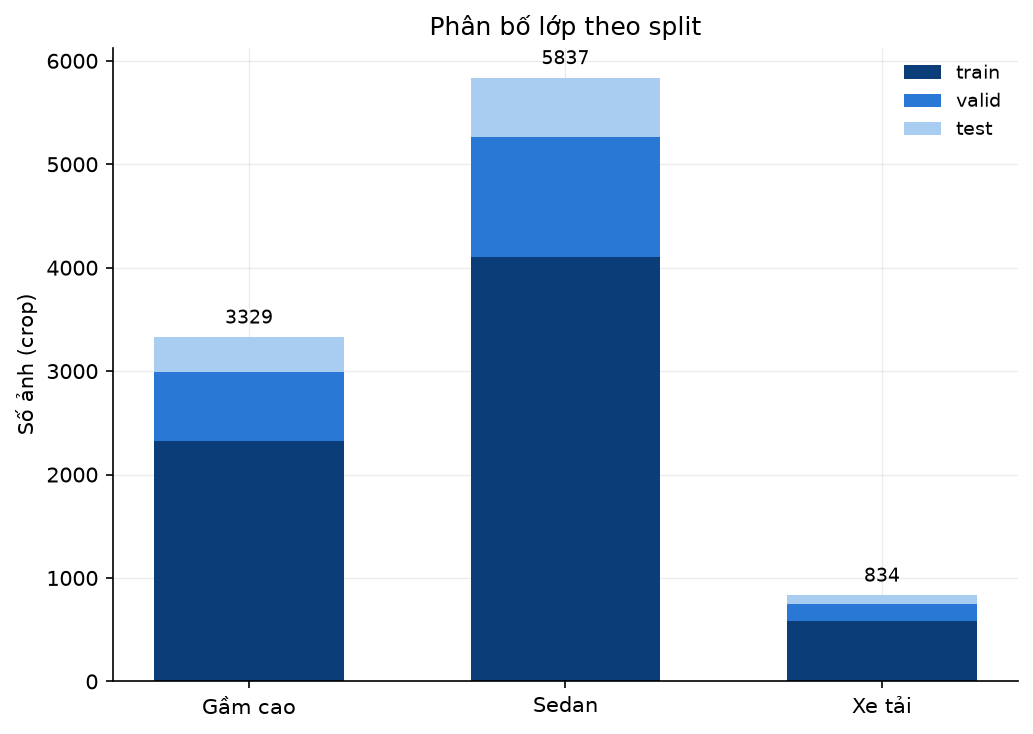
\includegraphics[width=0.90\textwidth]{vehicle_style_class_distribution.png}
\caption{Phân bố lớp theo split trong bộ dữ liệu B5 sau khi gộp.}
\label{fig:phanloai-phanboo}

\end{figure}

\section{Kiến Trúc và Huấn Luyện}
\label{sec:phanloai-kientruc}

Cả hai bước phân loại so sánh hai kiến trúc fine-tune từ trọng số ImageNet, thay lớp cuối cho
ba lớp: ResNet18~\autocite{he2016resnet} (khoảng 11,2 triệu tham số) và
MobileNetV3-Small~\autocite{howard2019mobilenetv3} (khoảng 1,5 triệu tham số, nhẹ hơn khoảng
7,3 lần). Điểm khác biệt là đầu vào: bước loại xe dùng \textbf{cả khung hình} (resize
224$\times$224) vì dữ liệu huấn luyện là ảnh camera cổng nguyên khung, còn bước kiểu dáng
dùng \textbf{vùng xe đã cắt} vì huấn luyện trên ảnh B5 cắt theo bounding box. Bước định vị
dùng YOLOv8n pretrained COCO~\autocite{jocher2023yolov8}, lấy bounding box xe lớn nhất kèm
biên 10\%.

Cả hai bước dùng chung cấu hình huấn luyện (Bảng~\ref{tab:app-cls}), mỗi mô hình dưới 7 phút
trên GPU; đường hội tụ nhanh và ổn định (Hình~\ref{fig:phanloai-losscurves}).

\begin{figure}[htbp]
\centering
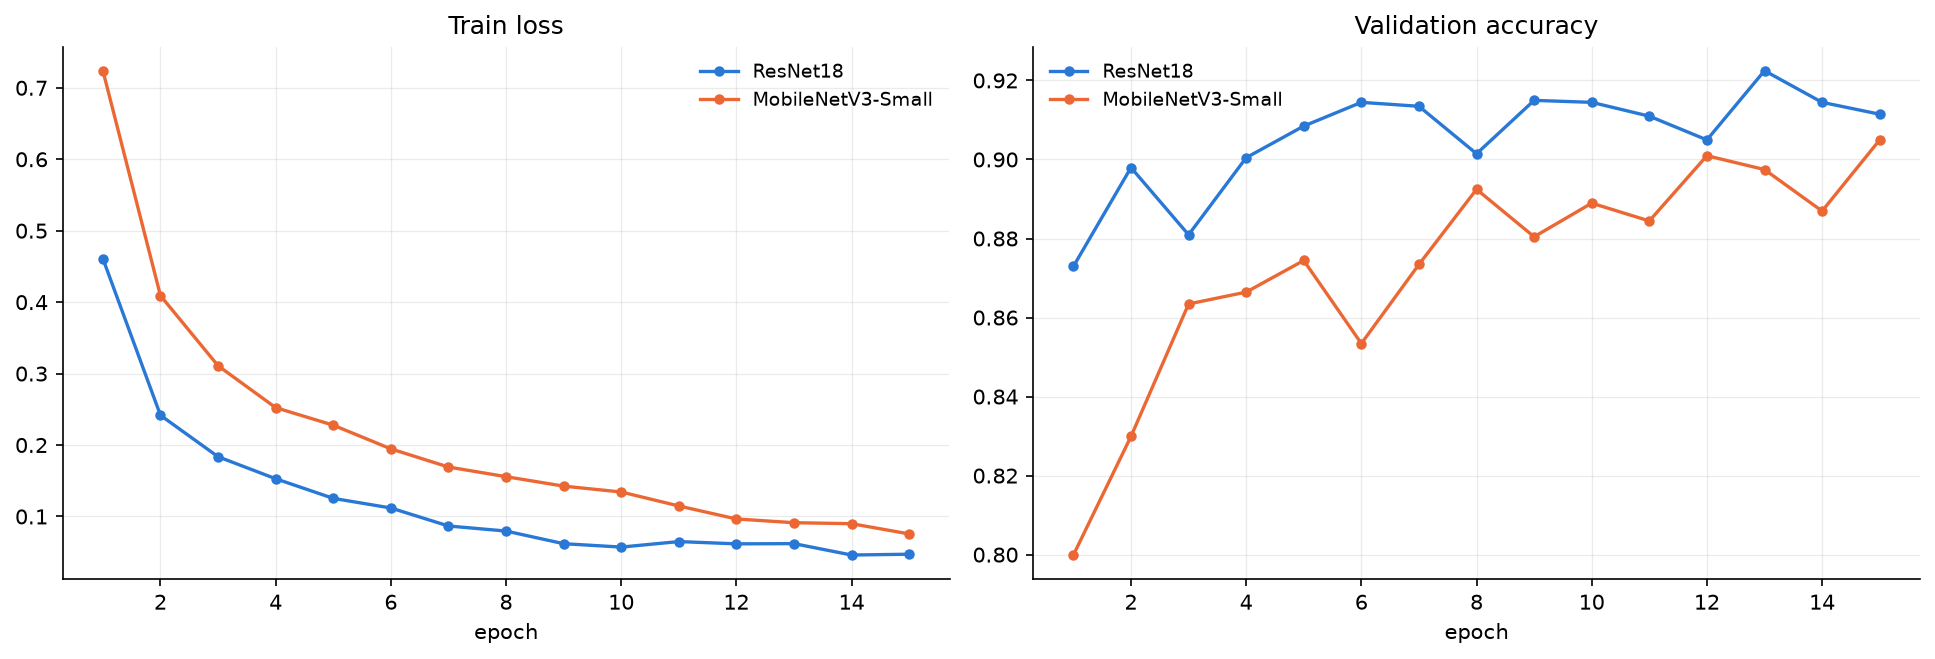
\includegraphics[width=0.90\textwidth]{vehicle_style_loss_curves.png}
\caption{Đường mất mát huấn luyện và accuracy kiểm định theo epoch của hai kiến trúc (bước kiểu dáng).}
\label{fig:phanloai-losscurves}

\end{figure}

\section{Kết Quả}
\label{sec:phanloai-ketqua}

\subsection{Bước loại xe}

Đánh giá trên tập test 149 ảnh (67 ô tô, 71 xe máy, 11 xe tải) sau khi khắc phục lỗi học tắt
(Bảng~\ref{tab:vt-results}, chi tiết từng lớp ở Phụ lục~\ref{app:ketqualop}). Cả hai mô hình
gần như tuyệt đối với ô tô và xe máy; xe tải yếu nhất (9/11) vì ít ảnh nhất, và lỗi phân tán
đều sang hai lớp kia, không còn dấu hiệu học tắt.

\begin{table}[htbp]
\centering
\caption{So sánh ResNet18 và MobileNetV3-Small ở bước loại xe (tập test 149 ảnh).}
\label{tab:vt-results}
{\footnotesize CPU inference đo trên máy huấn luyện, không phải Raspberry Pi~5.}
\begin{tabular}{lrrrrr}
\toprule
\textbf{Model} & \textbf{Accuracy} & \textbf{F1-macro} & \textbf{Params} & \textbf{ONNX} & \textbf{CPU inference} \\
\midrule
ResNet18 & 0,9866 & 0,9619 & 11,2 tr & 44,7 MB & 8,19 ms \\
MobileNetV3-Small & 0,9799 & 0,9571 & 1,5 tr & 6,1 MB & 4,22 ms \\
\bottomrule
\end{tabular}
\end{table}

Để xác nhận lỗi học tắt đã khắc phục tận gốc, đề tài dựng một bộ kiểm tra cố định gồm 12 ảnh
thật ngoài mọi tập train, valid và test: ResNet18 đúng 12/12 (100\%), MobileNetV3-Small 11/12
(92\%), so với chỉ 1/13 ở lần huấn luyện mắc lỗi học tắt.

Accuracy trên đây là của riêng mô hình. Khi ghép vào pipeline, nếu đặt bước định vị YOLO làm
điều kiện chạy thì detector pretrained bỏ sót 57\% ảnh cận cảnh camera cổng. Vì vậy đề tài cho mô hình loại xe chạy trên cả khung hình (đúng như dữ liệu
huấn luyện), chỉ dùng bằng chứng có xe (thấy xe hoặc đọc được biển) làm điều kiện an toàn;
nhờ đó tỉ lệ ảnh có kết quả đạt 100\% và độ chính xác end-to-end đạt 98,7\%, khớp đúng
accuracy của mô hình. Xe khách, chưa có lớp riêng, hiện do nhân viên sửa tay.

\subsection{Bước kiểu dáng}

Đánh giá trên tập test B5 987 ảnh (Bảng~\ref{tab:phanloai-sosanh}, Hình~\ref{fig:phanloai-sosanh}).
So với bài toán 12 lớp thử trước đó, accuracy cải thiện rõ (ResNet18 từ 0,768 lên 0,900;
MobileNetV3-Small từ 0,701 lên 0,901); với ba lớp, MobileNetV3-Small gần như ngang ResNet18
dù nhẹ hơn 7,3 lần. Ma trận nhầm lẫn (Hình~\ref{fig:phanloai-confusion}) cho thấy Sedan và Xe
tải phân loại tốt (93,1\% đến 96,4\% tùy mô hình); nhầm lẫn tập trung ở Gầm cao (79,6\% với
ResNet18, 83,2\% với MobileNetV3-Small), chủ yếu bị đoán nhầm thành Sedan, hợp lý vì crossover
cỡ nhỏ đôi khi có dáng gần sedan.

\begin{table}[htbp]
\centering
\caption{So sánh ResNet18 và MobileNetV3-Small ở bước kiểu dáng (tập test B5, 987 ảnh).}
\label{tab:phanloai-sosanh}
{\footnotesize CPU inference đo trên máy huấn luyện, không phải Raspberry Pi~5.}
\begin{tabular}{lrrrrr}
\toprule
\textbf{Model} & \textbf{Accuracy} & \textbf{F1-macro} & \textbf{Params} & \textbf{ONNX} & \textbf{CPU inference} \\
\midrule
ResNet18 & 0,8997 & 0,9012 & 11,2 tr & 44,7 MB & 8,57 ms \\
MobileNetV3-Small & 0,9007 & 0,9069 & 1,5 tr & 6,1 MB & 4,82 ms \\
\bottomrule
\end{tabular}
\end{table}

\begin{figure}[htbp]
\centering
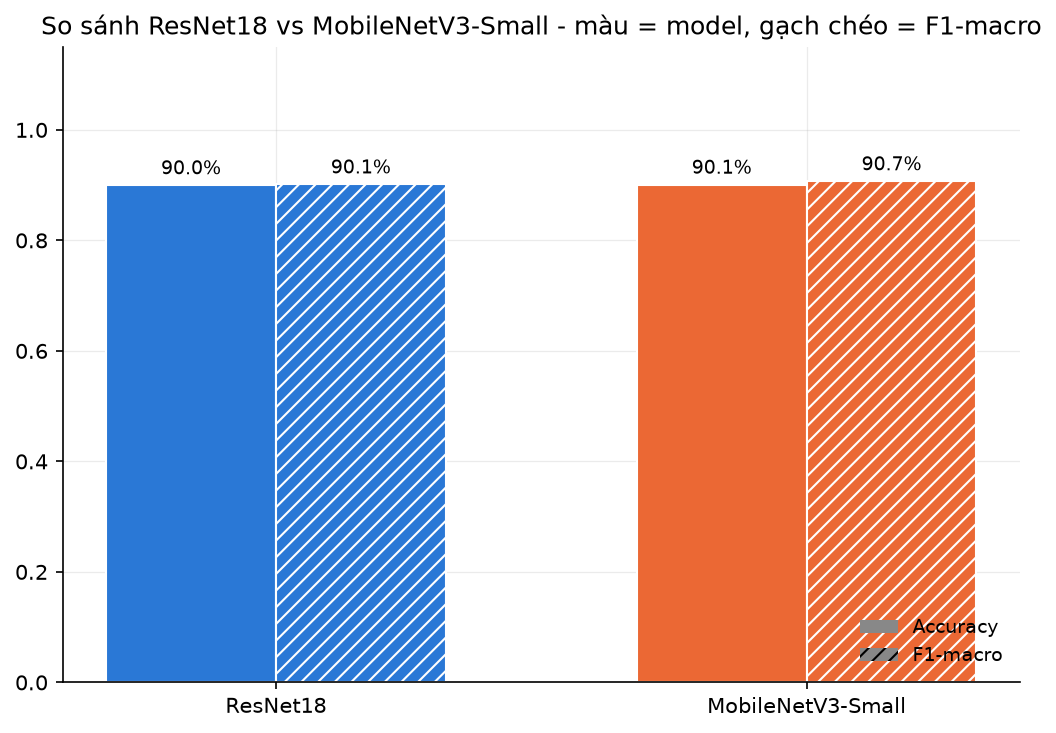
\includegraphics[width=0.90\textwidth]{vehicle_style_comparison.png}
\caption{So sánh tổng quan hai kiến trúc theo các chỉ số đánh giá (bước kiểu dáng).}
\label{fig:phanloai-sosanh}

\end{figure}

\begin{figure}[htbp]
\centering

\includegraphics[width=0.90\textwidth]{vehicle_style_confusion_matrices.png}
\caption{Ma trận nhầm lẫn trên tập test của ResNet18 và MobileNetV3-Small (bước kiểu dáng).}
\label{fig:phanloai-confusion}

\end{figure}

\section{Thảo Luận}
\label{sec:phanloai-thaoluan}

\textbf{Accuracy trên tập test nội bộ không đảm bảo hiệu năng thật.} Kết quả 1/13 trước và
12/12 sau khi trộn nguồn trên bộ ngoài phân phối cho thấy tập kiểm tra phải tách nguồn với
tập huấn luyện; độ đa dạng nguồn ảnh quan trọng hơn số lượng ảnh.

\textbf{Accuracy của mô hình không phải accuracy người dùng nhận được.} Khi ghép nhiều mô
hình, không nên để một thành phần chưa đánh giá (bước định vị YOLO, bỏ sót 57\% ảnh) chặn
đầu vào của thành phần đã có số liệu.

\textbf{Hạn chế còn lại.} YOLO pretrained COCO vẫn bỏ sót xe trên nhiều ảnh camera cổng; khi
đó hệ thống vẫn ra loại xe và biển số nhưng thiếu khung xe và kiểu dáng. Mô hình kiểu dáng
huấn luyện hoàn toàn trên ảnh đại lý của B5 nên con số 90\% chưa được kiểm chứng trên ảnh
camera cổng thật.

\textbf{Chọn mô hình triển khai.} Bước loại xe chọn ResNet18 vì chính xác hơn rõ (0,9866 so
với 0,9799 trên tập test, 100\% so với 92\% trên bộ ngoài phân phối). Bước kiểu dáng chọn
MobileNetV3-Small: hai kiến trúc gần ngang nhau về accuracy (0,8997 so với 0,9007) nhưng
MobileNetV3-Small nhẹ hơn 7,3 lần, giảm footprint và chạy mát hơn mà không giảm độ chính xác
đáng kể (đo trên Raspberry Pi~5 ở Chương~\ref{ch:trienkhai}).
       % Chương 6: Phân loại phương tiện
% =====================================================================
%  CHƯƠNG 7. HỆ THỐNG QUẢN LÝ BÃI GIỮ XE       | Phụ trách: Đức
%  Ngân sách: mục tiêu 6 trang. Viết high-level, không đi sâu vào mã nguồn.
%  Nội dung dựa trên thiết kế backend (FastAPI, PostgreSQL) và dashboard (React).
% =====================================================================
\chapter{Hệ Thống Quản Lý Bãi Giữ Xe}
\label{ch:hethong}

% -------------------------------------------------------------------
\section{Kiến Trúc Tổng Thể}
\label{sec:kientruc}
% -------------------------------------------------------------------

Hệ thống tổ chức theo ba lớp: thu nhận ảnh tại cổng, backend xử lý nghiệp vụ, và cơ sở dữ
liệu. Điểm khác biệt là hai đường thu nhận ảnh song song cùng đổ về một backend duy nhất và
dùng chung một bộ suy luận (Hình~\ref{fig:kientruc}). Đường thứ nhất là kiosk trên máy tính:
giao diện cổng chụp ảnh từ webcam, gửi lên backend để suy luận ngay trong tiến trình và trả
kết quả. Đường thứ hai là cổng tự động trên thiết bị biên: worker chạy suy luận tại chỗ rồi
gửi kết quả kèm ảnh về backend, backend không suy luận lại mà chỉ ghi nhận và xử lý nghiệp
vụ. Cả hai đường dùng chung một pipeline nhận diện, nên kết quả nhất quán bất kể ảnh được xử
lý ở đâu.

\begin{figure}[htbp]
\centering
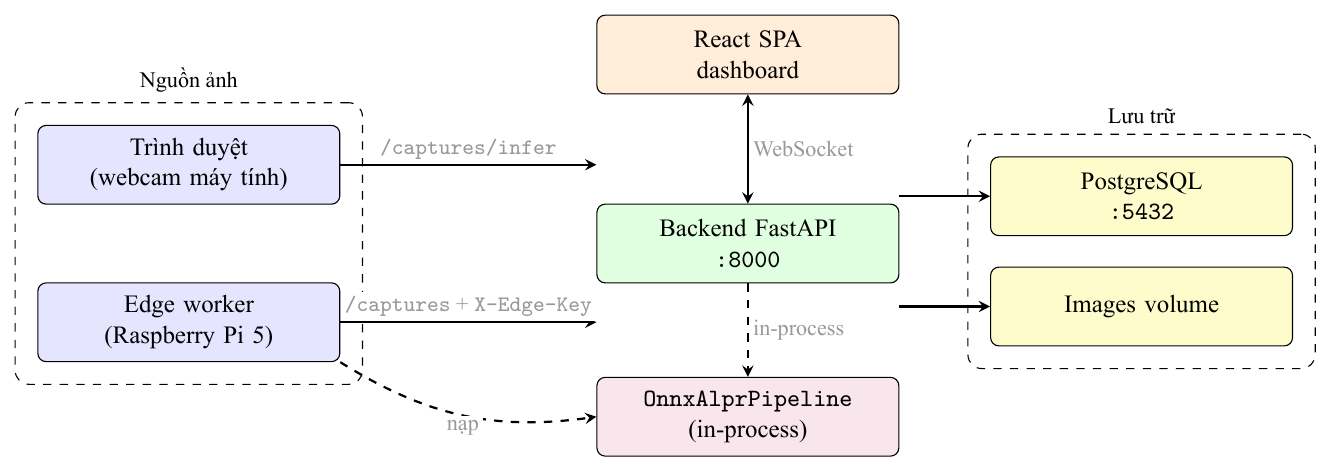
\includegraphics[width=0.9\textwidth]{uml-kientruc.png}
\caption{Kiến trúc tổng thể hệ thống: hai đường thu nhận ảnh cùng đổ về một backend.}
\label{fig:kientruc}

\end{figure}

Cùng một bộ mã chạy trên hai cấu hình triển khai, chọn qua cấu hình mà không sửa mã
(Bảng~\ref{tab:cauhinh-trienkhai}): trên máy tính, các thành phần chạy trong container với
PostgreSQL; trên Raspberry Pi~5, backend và giao diện chạy trực tiếp trên hệ điều hành với
SQLite và tăng số luồng suy luận để tận dụng bốn nhân.

\begin{table}[htbp]
\centering
\caption{Hai cấu hình triển khai của hệ thống.}
\label{tab:cauhinh-trienkhai}

\vspace{4pt}
\begin{tabular}{lll}
\toprule
\textbf{Thành phần} & \textbf{Máy tính} & \textbf{Raspberry Pi 5} \\
\midrule
Backend & Container FastAPI & FastAPI chạy trực tiếp \\
Cơ sở dữ liệu & PostgreSQL & SQLite \\
Phát hiện biển số & YOLOv8n & YOLOv8n \\
Đọc ký tự, loại xe, kiểu dáng & ONNX Runtime & ONNX Runtime \\
Số luồng mỗi mô hình & 1 & 4 \\
\bottomrule
\end{tabular}
\end{table}

Pipeline nạp các mô hình một lần khi khởi động rồi chạy trọn chuỗi nhận diện
(Mục~\ref{sec:donggop}) trên mỗi khung ảnh; nhờ tách khỏi lớp vận chuyển, cùng một pipeline
phục vụ cả kiosk lẫn worker biên.

% -------------------------------------------------------------------
\section{Cơ Sở Dữ Liệu}
\label{sec:csdl}
% -------------------------------------------------------------------

Cơ sở dữ liệu tổ chức quanh tám thực thể trung tâm (Bảng~\ref{tab:bang-chinh}), với sơ đồ
quan hệ ở Hình~\ref{fig:uml-er}. Ngoài ra còn các bảng hỗ trợ cho nhóm xe và bảng giá, vé
tháng, danh sách trắng và đen, sự cố, thiết bị cổng và cấu hình bãi.

\begin{table}[htbp]
\centering
\caption{Các thực thể trung tâm trong cơ sở dữ liệu.}
\label{tab:bang-chinh}

\vspace{4pt}
\begin{tabular}{lp{9.5cm}}
\toprule
\textbf{Thực thể} & \textbf{Vai trò} \\
\midrule
Phiên gửi xe & Vòng đời một lượt gửi xe: trạng thái, phí chốt và bản ghi quy tắc giá tại thời điểm chốt \\
Lượt đọc biển & Một lần đọc biển tại cổng (vào hoặc ra), lưu kết quả nhận diện và trạng thái duyệt \\
Thanh toán & Giao dịch thu tiền, hoàn trả hoặc điều chỉnh theo ca trực \\
Quy tắc giá & Bảng giá theo nhóm xe: chế độ tính, đơn giá, khối thời gian, thời gian miễn phí, mức trần ngày \\
Ảnh bằng chứng & Ảnh toàn cảnh và ảnh cắt biển; trạng thái mã hóa và thời hạn xóa \\
Ca trực & Ca làm việc của nhân viên, gắn với các giao dịch thu tiền \\
Người dùng & Tài khoản và vai (nhân viên, quản lý, quản trị) \\
Nhật ký kiểm toán & Ghi lại các thao tác nhạy cảm để đối soát sau sự cố \\
\bottomrule
\end{tabular}
\end{table}

\begin{figure}[htbp]
\centering
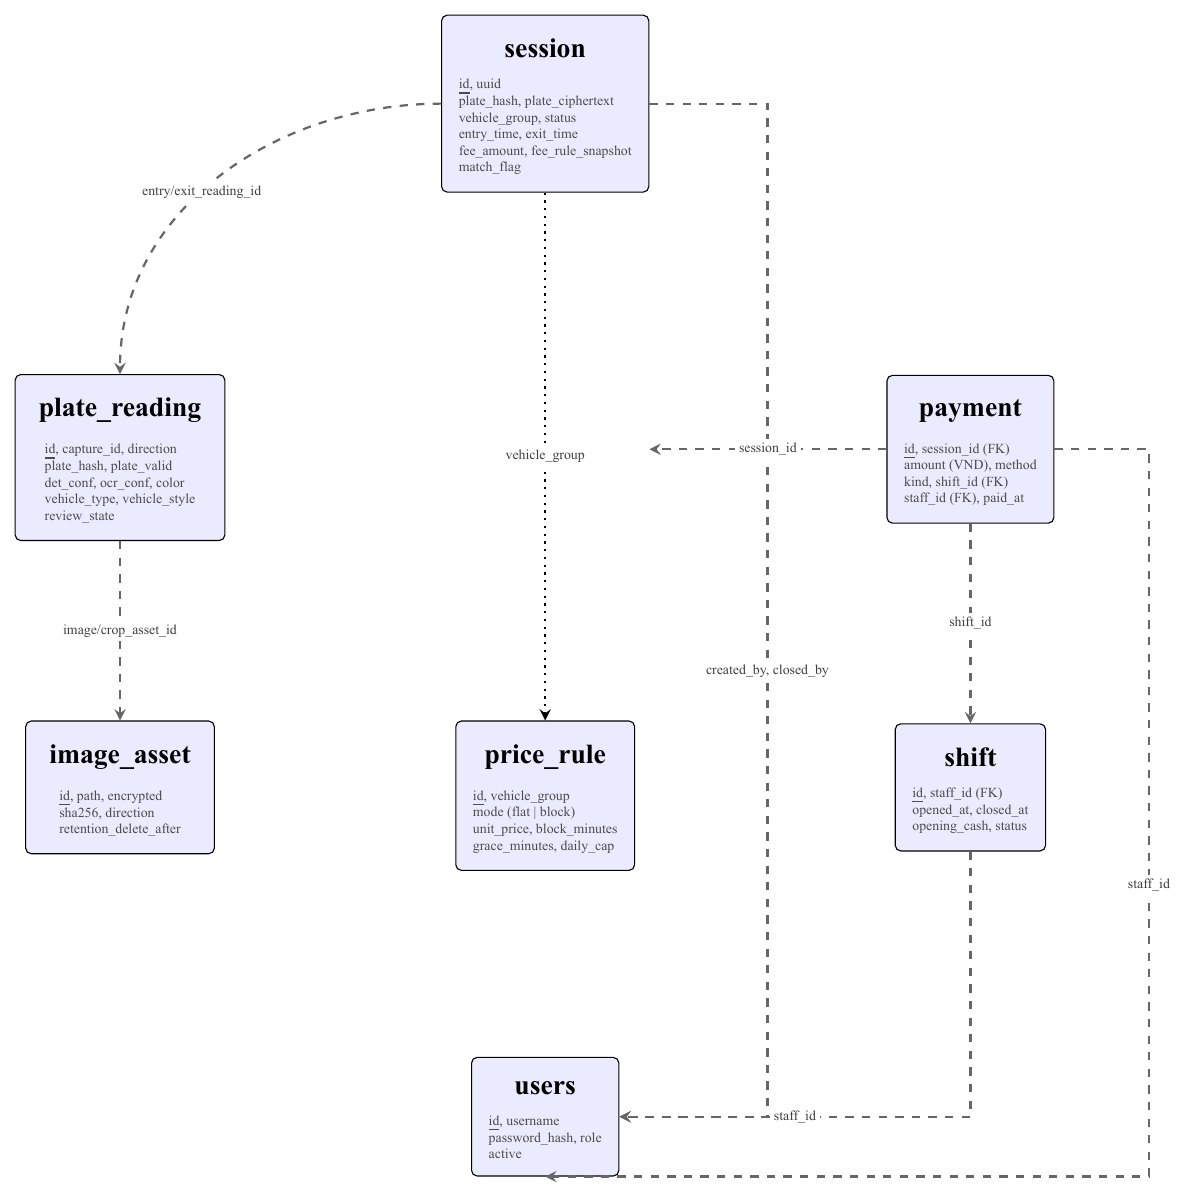
\includegraphics[width=0.9\textwidth]{uml-er.png}
\caption{Sơ đồ quan hệ thực thể của các bảng trung tâm.}
\label{fig:uml-er}

\end{figure}

\textbf{Bảo mật dữ liệu cá nhân.} Biển số và ảnh phương tiện là dữ liệu cá nhân theo Luật Bảo
vệ dữ liệu cá nhân~\autocite{vn2025lutbvdlcn}. Mỗi chuỗi biển được lưu đồng thời dạng băm (để
đối chiếu) và dạng mã hóa (để hiển thị khi có quyền); ảnh bằng chứng được mã hóa và chỉ truy
cập qua endpoint có kiểm tra quyền; một tiến trình nền xóa dữ liệu quá hạn tính từ lúc xe ra.
Đối chiếu đầy đủ với nghĩa vụ theo luật ở Phụ lục~\ref{app:baomat}.

% -------------------------------------------------------------------
\section{Logic Vào Ra và Chống Gian Lận}
\label{sec:logic-vaora}
% -------------------------------------------------------------------

Mỗi phiên gửi xe đi qua các trạng thái: đang trong bãi, chờ xử lý thủ công (khi không đọc
được biển), hoàn thành, và tranh chấp. Khi xe vào, hệ thống tạo phiên mới và cảnh báo nếu
biển trùng một phiên đang trong bãi hoặc nằm trong danh sách đen.

Khi xe ra, hệ thống đối chiếu biển theo ba cấp (Hình~\ref{fig:uml-seq}). Trước hết là khớp
chính xác qua giá trị băm; nếu không khớp, hệ thống so khoảng cách chỉnh sửa giữa chuỗi biển
ra và các phiên đang trong bãi cùng nhóm xe, chấp nhận khi lệch không quá một ký tự (xử lý
sai sót nhỏ của OCR); nếu vẫn không rõ ràng, hệ thống đưa danh sách ứng viên cho nhân viên
chọn hoặc chuyển phiên sang trạng thái tranh chấp. Mỗi lượt đọc đều gắn ảnh toàn cảnh và ảnh
cắt biển làm bằng chứng khi cần đối soát; trường hợp mất vé được xử lý thành phiên riêng có
phí phạt và ghi nhật ký.

\begin{figure}[htbp]
\centering
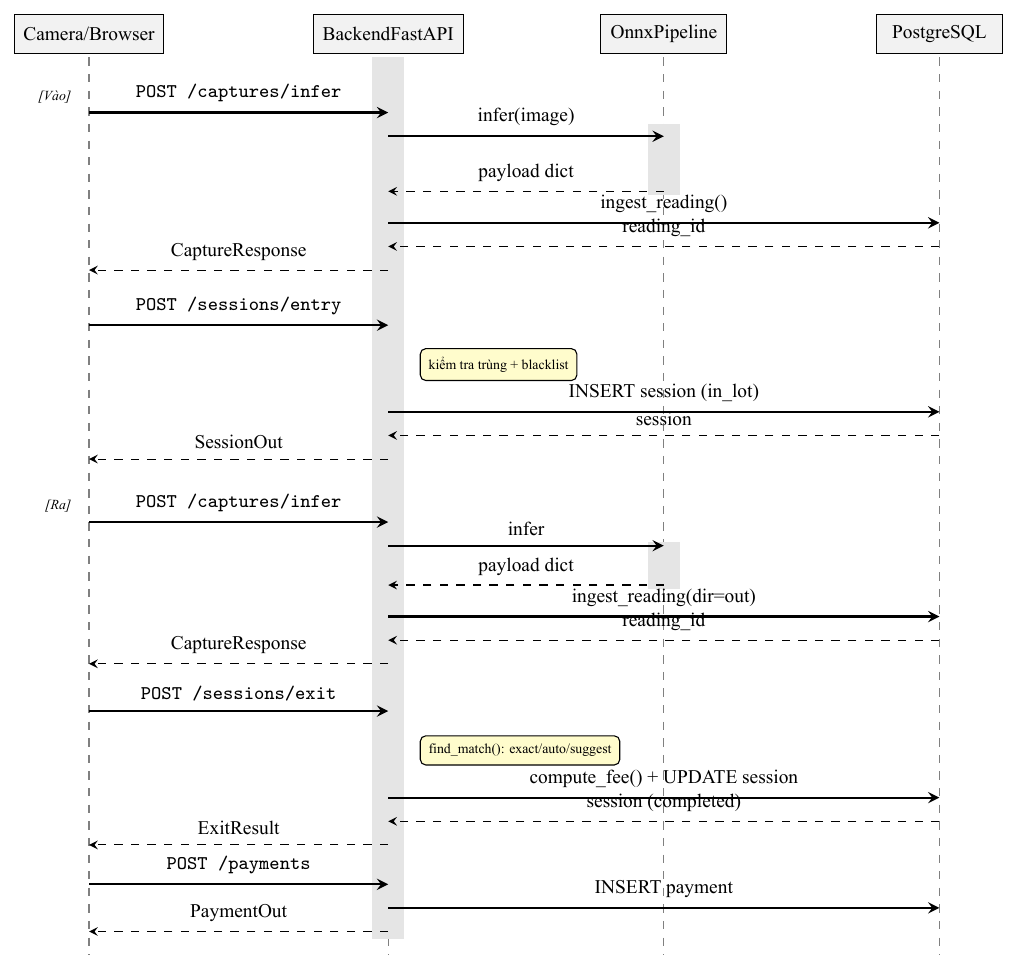
\includegraphics[width=0.9\textwidth]{uml-seq.png}
\caption{Sơ đồ tuần tự một lượt xe từ vào đến ra: thu nhận ảnh, tạo phiên, đối chiếu biển, tính phí và ghi thanh toán.}
\label{fig:uml-seq}

\end{figure}

% -------------------------------------------------------------------
\section{Tính Phí Tự Động}
\label{sec:tinphi}
% -------------------------------------------------------------------

Mỗi nhóm xe (xe máy, ô tô con, xe tải, xe khách) có một quy tắc giá đang kích hoạt. Hệ thống
hỗ trợ hai chế độ: chế độ phẳng thu cố định mỗi lượt, và chế độ theo khối thời gian nhân đơn
giá với số khối làm tròn lên, có thể chặn tại mức trần theo ngày. Khoảng thời gian miễn phí
đầu (grace period) cho phép ra trong ít phút mà không mất phí. Khi phiên kết thúc, toàn bộ
quy tắc được chốt kèm phiên tại thời điểm đó, nên thay đổi bảng giá về sau không ảnh hưởng
phí đã tính của các phiên cũ và vẫn đối soát được. Xe thuộc danh sách miễn phí được ghi rõ
lý do miễn để phân biệt với phí thật sự bằng không.

% -------------------------------------------------------------------
\section{Dashboard Quản Lý và Thống Kê}
\label{sec:dashboard}
% -------------------------------------------------------------------

Hệ thống phân ba vai người dùng cùng một tác nhân thiết bị biên
(Bảng~\ref{tab:vaitro}, sơ đồ use case ở Hình~\ref{fig:uml-usecase}). Nhân viên xử lý nghiệp
vụ cổng; quản lý thêm quyền cấu hình bảng giá, tra cứu thống kê và xuất dữ liệu; quản trị
quản lý tài khoản. Thiết bị biên là tác nhân riêng, xác thực bằng khóa riêng thay vì tài
khoản người dùng.

\begin{table}[htbp]
\centering
\caption{Các tác nhân và quyền chính trong hệ thống.}
\label{tab:vaitro}

\vspace{4pt}
\begin{tabular}{lp{9.5cm}}
\toprule
\textbf{Tác nhân} & \textbf{Quyền chính} \\
\midrule
Nhân viên & Chụp và nhận diện, xác nhận vào ra, thu tiền, sửa biển, mở và chốt ca, tra cứu phiên \\
Quản lý & Toàn bộ quyền nhân viên; bảng giá, nhóm xe, vé tháng, danh sách trắng và đen, giải quyết tranh chấp, thống kê và xuất CSV, tạo tài khoản nhân viên \\
Quản trị & Toàn bộ quyền quản lý; quản lý tài khoản vai quản lý và quản trị \\
Thiết bị biên & Gửi kết quả nhận diện kèm ảnh và tín hiệu hoạt động; xác thực bằng khóa riêng \\
\bottomrule
\end{tabular}
\end{table}

\begin{figure}[htbp]
\centering
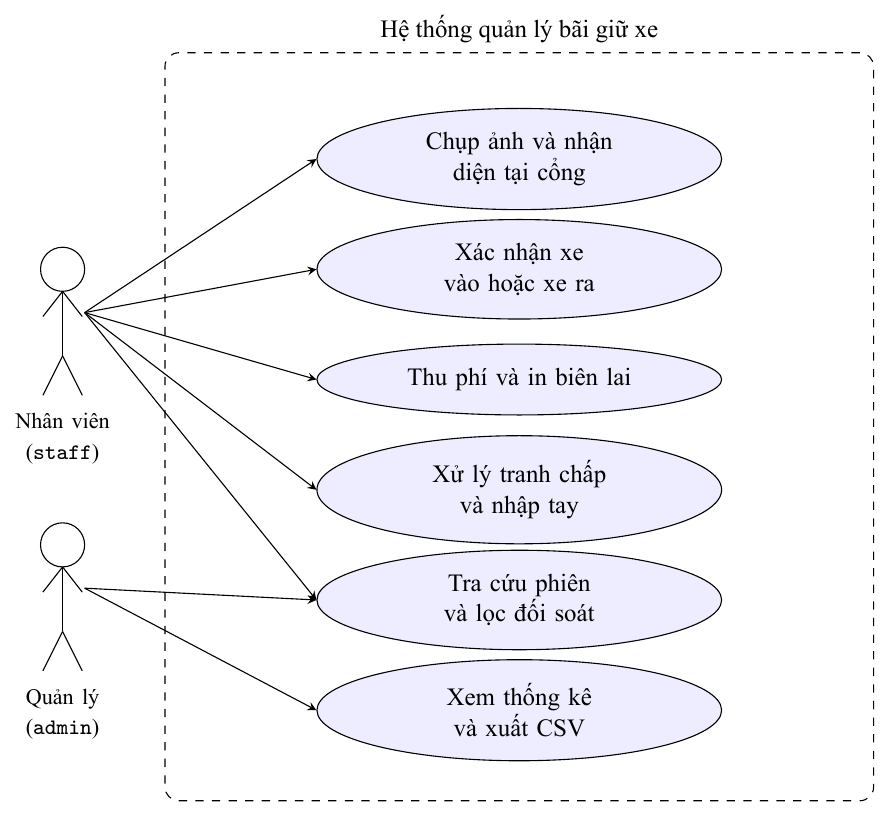
\includegraphics[width=0.9\textwidth]{uml-usecase.png}
\caption{Sơ đồ use case: nhân viên thực hiện nghiệp vụ cổng, quản lý thêm quyền cấu hình và thống kê.}
\label{fig:uml-usecase}

\end{figure}

Giao diện gồm bốn nhóm màn hình chính. Màn cổng chia khung vào và khung ra, hiển thị kết quả
nhận diện theo thời gian thực: biển số, loại xe, màu nền, ảnh biển đã xử lý và phí đề xuất
(Hình~\ref{fig:dash-gate-in}); khi xe ra, khung ra đặt ảnh lúc vào cạnh ảnh lúc ra để đối
chiếu trước khi thu phí (Hình~\ref{fig:dash-gate-out}). Trang tra cứu phiên lọc theo nhóm xe,
thời gian, trạng thái và cách khớp biển (Hình~\ref{fig:dash-sessions}); trang chi tiết giữ
ảnh bằng chứng của cả hai lượt cùng phí và quy tắc giá lúc chốt
(Hình~\ref{fig:dash-detail}). Trang thống kê tổng hợp số xe vào ra và doanh thu theo ngày,
kèm xuất CSV (Hình~\ref{fig:dash-stats}). Trang cấu hình quản lý bảng giá, tài khoản và công
tắc các bước AI, đồng thời nêu rõ chính sách tự xóa dữ liệu phiên sau thời hạn quy định
(Hình~\ref{fig:dash-config}).

\begin{figure}[htbp]
\centering
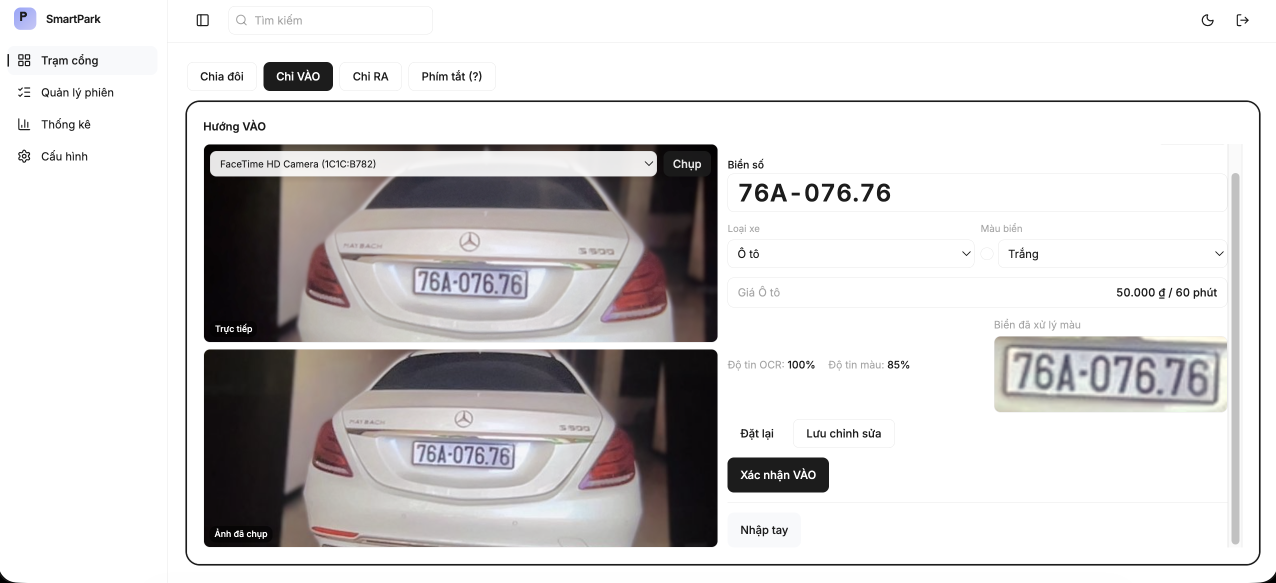
\includegraphics[width=0.92\textwidth]{dashboard-gate-in.png}
\caption{Màn cổng, khung vào: kết quả nhận diện thời gian thực gồm biển số, loại xe, màu nền, ảnh biển đã xử lý và phí đề xuất.}
\label{fig:dash-gate-in}

\end{figure}

\begin{figure}[htbp]
\centering
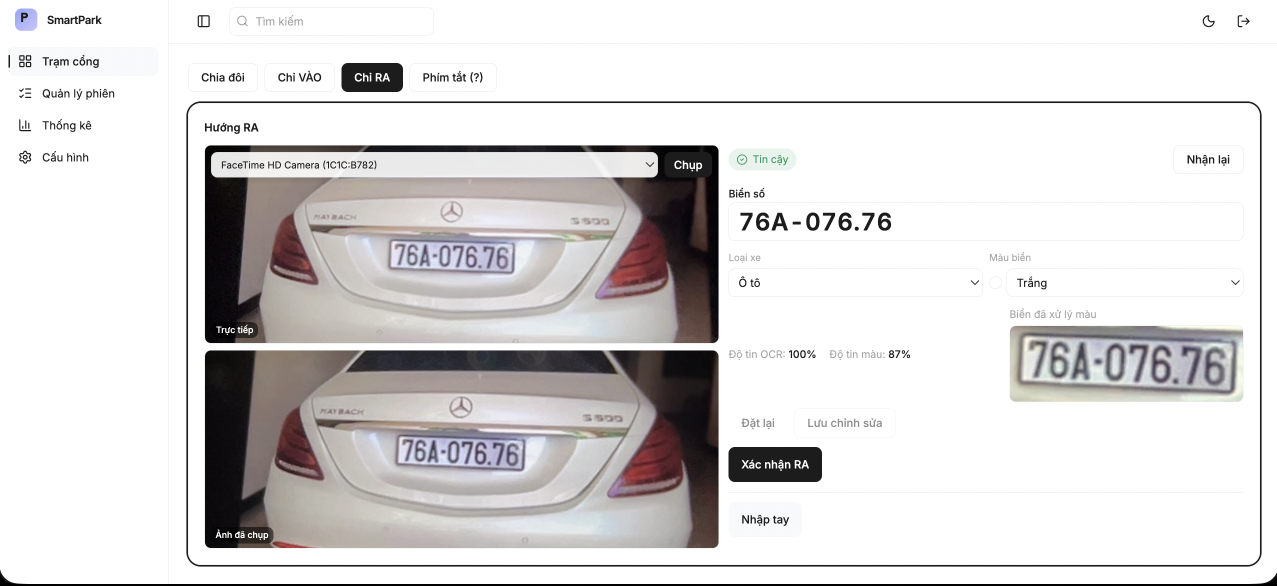
\includegraphics[width=0.92\textwidth]{dashboard-gate-out.png}
\caption{Khung ra đối chiếu ảnh lúc vào và lúc ra của cùng một xe trước khi thu phí.}
\label{fig:dash-gate-out}

\end{figure}

\begin{figure}[htbp]
\centering
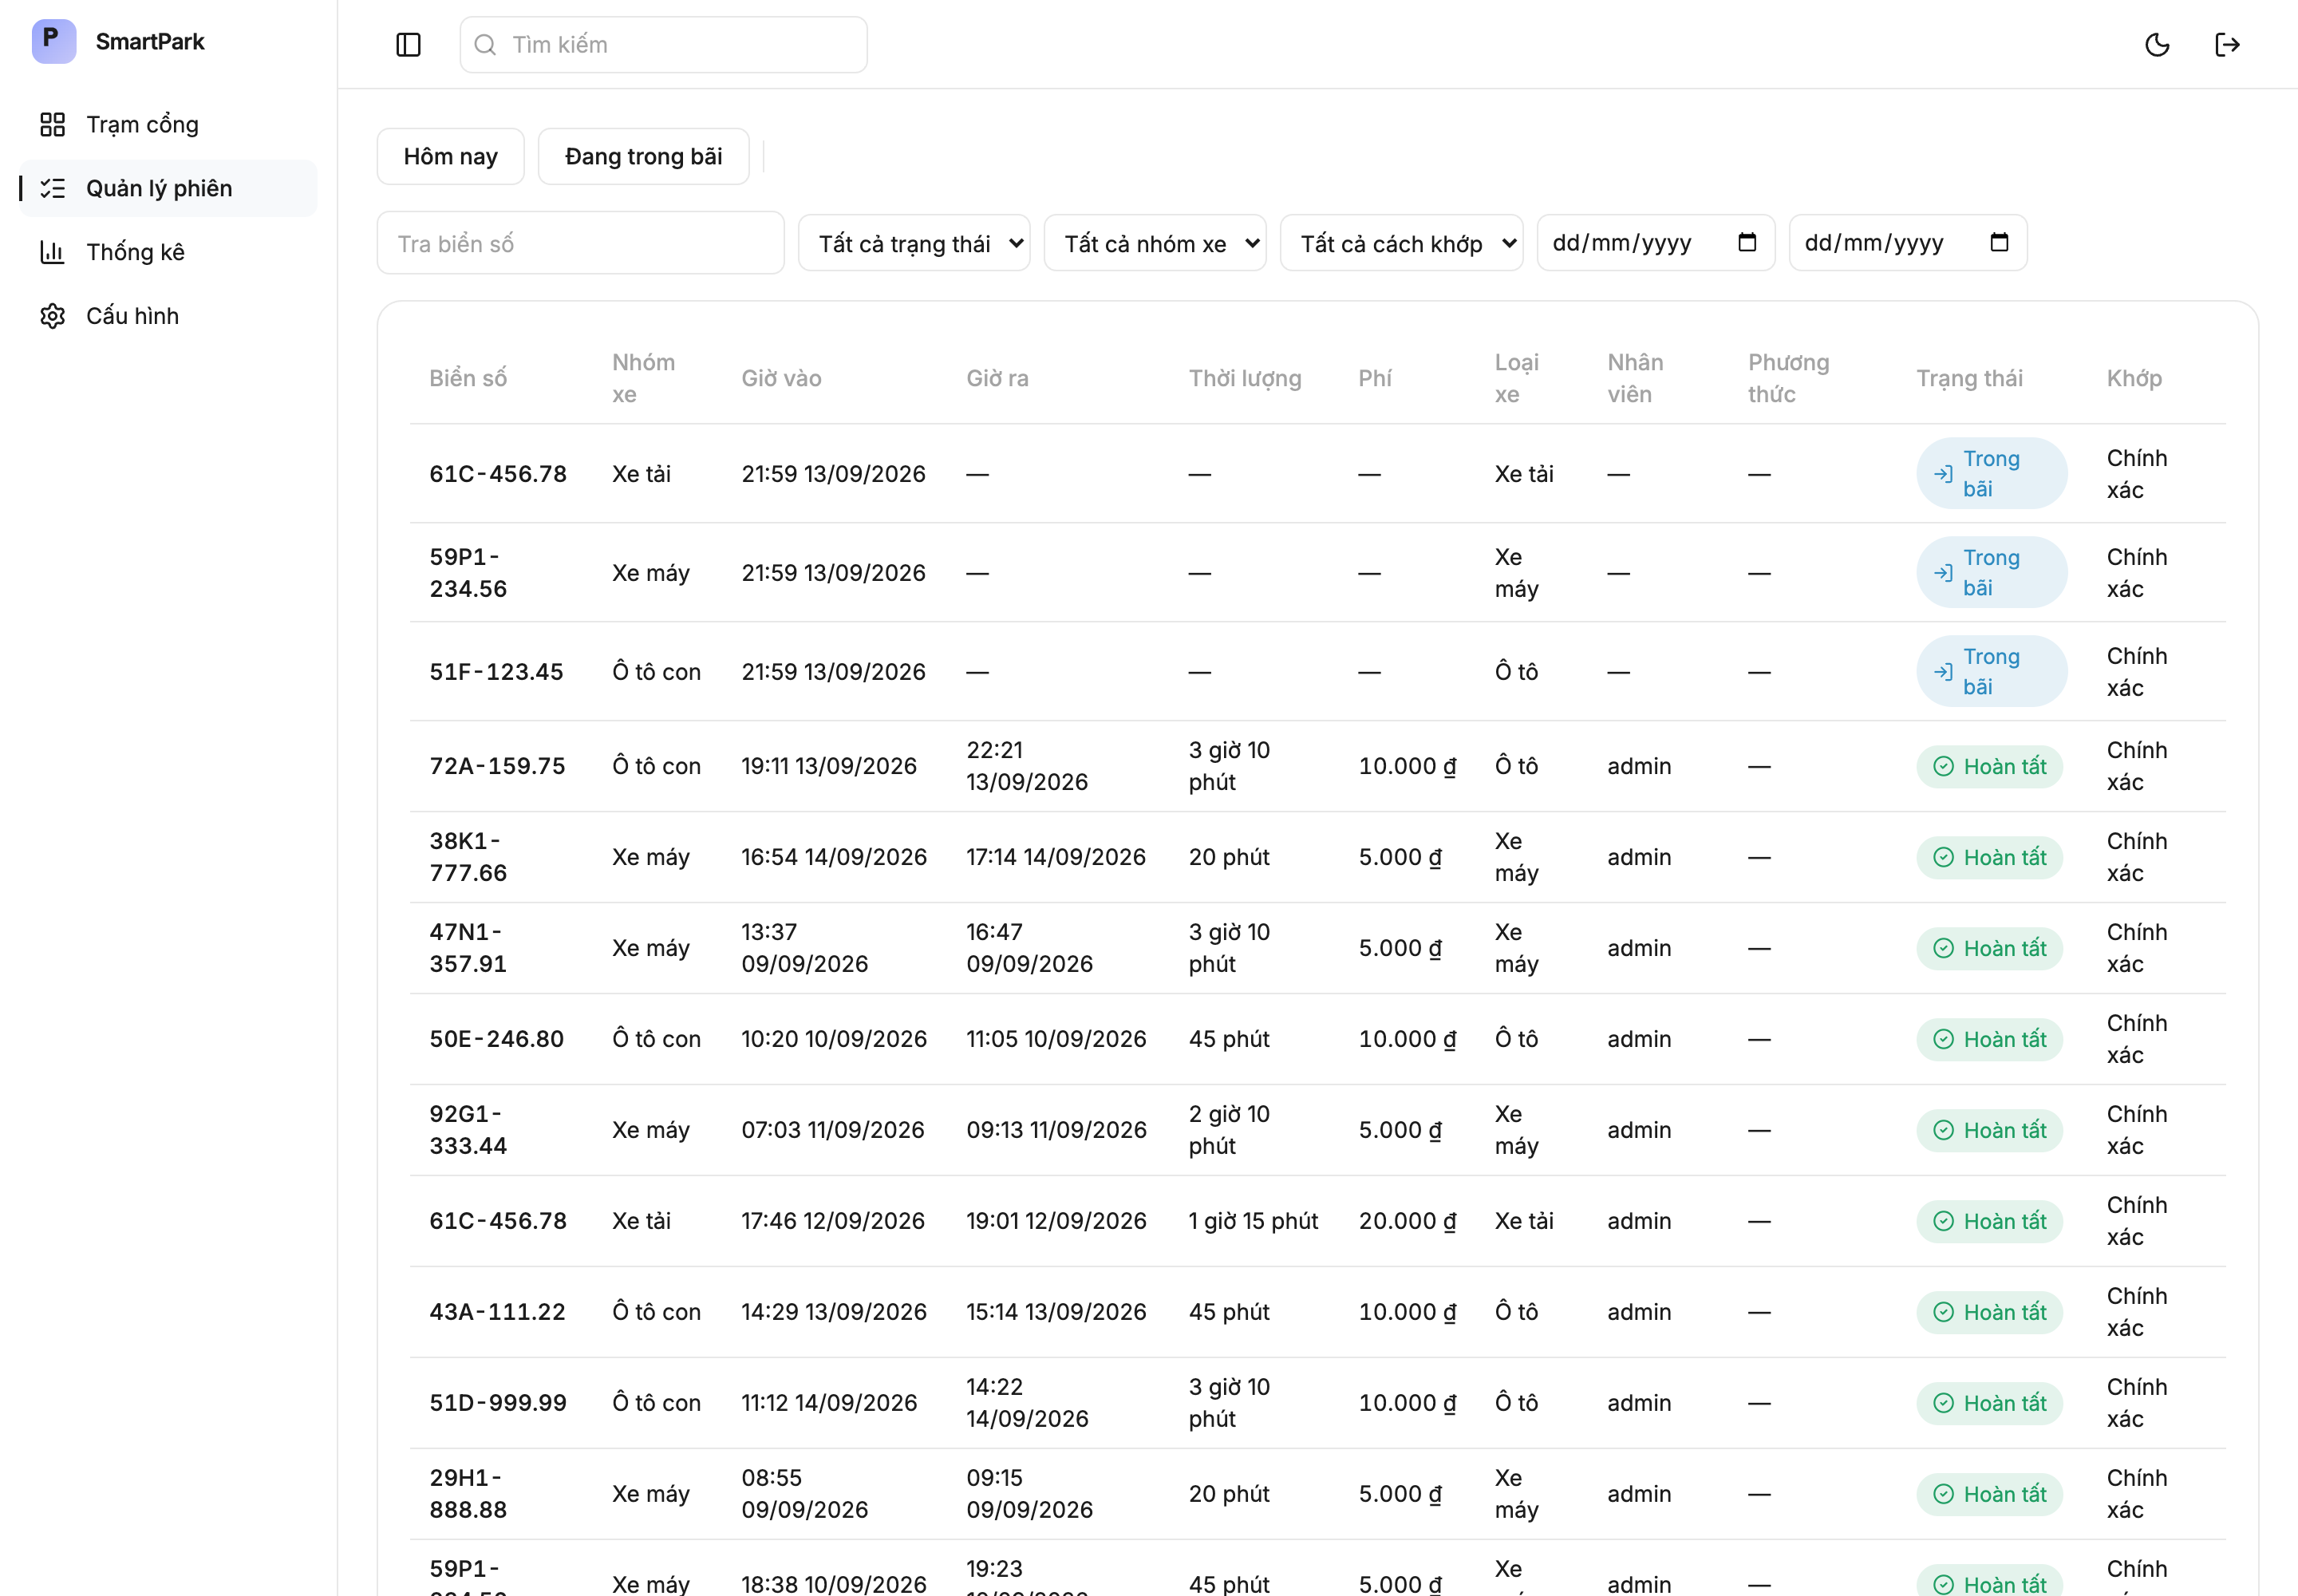
\includegraphics[width=0.95\textwidth]{dashboard-sessions.png}
\caption{Trang tra cứu phiên: bộ lọc và danh sách phiên với biển số, thời gian vào ra, phí, cách khớp và trạng thái.}
\label{fig:dash-sessions}

\end{figure}

\begin{figure}[htbp]
\centering
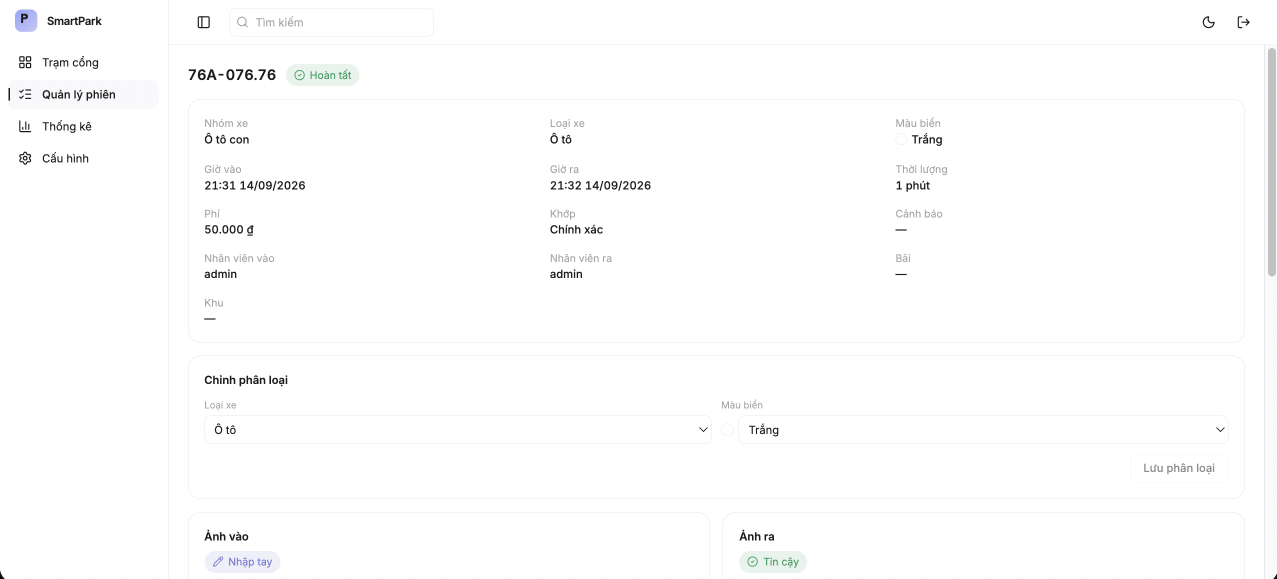
\includegraphics[width=0.92\textwidth]{dashboard-session-detail.png}
\caption{Chi tiết một phiên gửi xe: thông tin phiên, phân loại và ảnh bằng chứng lúc vào, lúc ra.}
\label{fig:dash-detail}

\end{figure}

\begin{figure}[htbp]
\centering
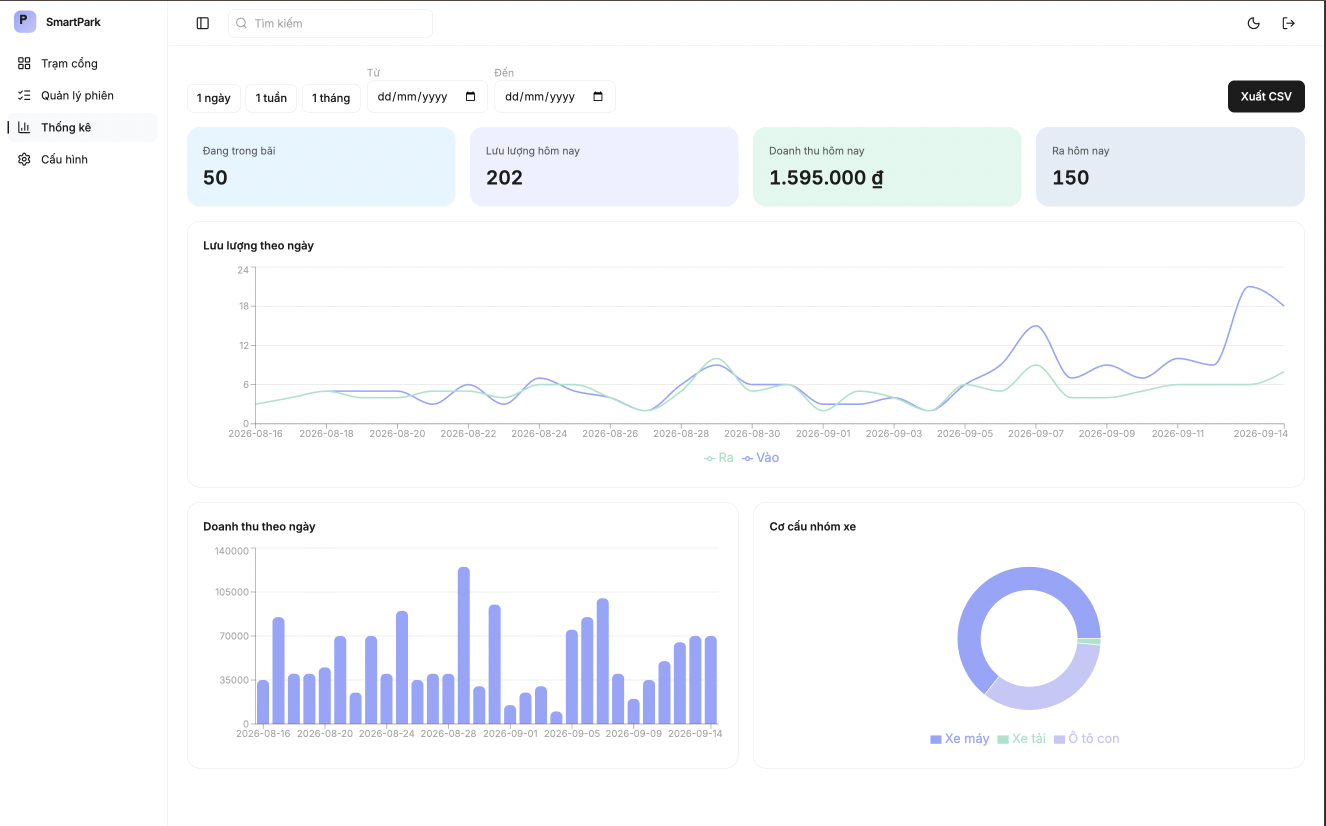
\includegraphics[width=0.95\textwidth]{dashboard-stats-new.png}
\caption{Trang thống kê: thẻ tổng hợp, biểu đồ lưu lượng và doanh thu theo ngày, nút xuất CSV.}
\label{fig:dash-stats}

\end{figure}

\begin{figure}[htbp]
\centering
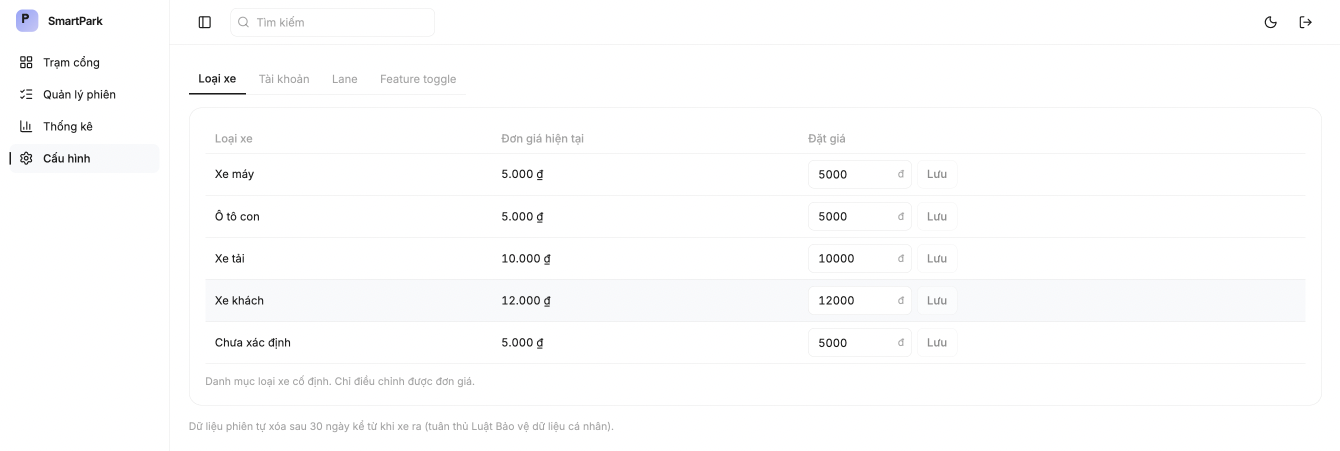
\includegraphics[width=0.95\textwidth]{dashboard-config.png}
\caption{Trang cấu hình bảng giá theo nhóm xe, kèm ghi chú tự xóa dữ liệu phiên theo Luật Bảo vệ dữ liệu cá nhân.}
\label{fig:dash-config}

\end{figure}
        % Chương 7: Hệ thống quản lý bãi giữ xe
% =====================================================================
%  CHƯƠNG 8 — TRIỂN KHAI THIẾT BỊ BIÊN VÀ ĐÁNH GIÁ
%  Phụ trách: Nhật (tối ưu mô hình) + Đức (đóng gói, worker)
%  Viết high-level, không nhắc mã nguồn/hàm/đường dẫn.
%  INT8: CHƯA thực hiện — chỉ nêu ở hướng phát triển (Chương 9).
%  Số Pi5 đo trực tiếp ngày 2026-09-13.
% =====================================================================
\chapter{Triển Khai Trên Thiết Bị Biên và Đánh Giá}
\label{ch:trienkhai}

\section{Nền Tảng Phần Cứng Mục Tiêu}
\label{sec:trienkhai-phancung}

Raspberry Pi 5 được chọn vì CPU bốn nhân Cortex-A76 đủ chạy YOLO cỡ nano qua ONNX Runtime mà
không cần GPU rời (Mục~\ref{sec:pi5bench}), chi phí thấp và có sẵn giao tiếp camera CSI lẫn
GPIO. Mọi mô hình được huấn luyện trên máy tính có GPU; các phép đo hiệu năng chạy
trên CPU của cả hai máy để so cùng điều kiện (Bảng~\ref{tab:moi-truong}).

\begin{table}[htbp]
\centering
\caption{Cấu hình phần cứng và phần mềm dùng trong thực nghiệm.}
\label{tab:moi-truong}

\vspace{4pt}
\begin{tabular}{lll}
\toprule
\textbf{Thành phần} & \textbf{Máy tính} & \textbf{Raspberry Pi 5} \\
\midrule
CPU          & Intel Core i7-13700K (16 nhân, 24 luồng) & 4 nhân Cortex-A76 2,4 GHz \\
Bộ nhớ       & 64 GB & 16 GB \\
GPU          & NVIDIA RTX 4070 (chỉ khi huấn luyện) & Không \\
Hệ điều hành & Windows 11 Pro & Debian GNU/Linux 13, kernel 6.18 \\
ONNX Runtime & 1.28 & 1.30 \\
Backend      & FastAPI, PostgreSQL & FastAPI, SQLite \\
\bottomrule
\end{tabular}
\end{table}

\section{Tối Ưu và Đóng Gói Mô Hình}
\label{sec:trienkhai-toiuu}

Ba mô hình đọc ký tự, phân loại loại xe và phân loại kiểu dáng chạy dưới ONNX Runtime, không
phụ thuộc PyTorch khi suy luận; các detector biển số và định vị xe chạy qua Ultralytics. Bản
ONNX cho dự đoán trùng khớp bản huấn luyện (Mục~\ref{sec:ocr-charset37}) và chạy được trên CPU
ARM, macOS lẫn Windows, nên cùng một mô hình dùng chung cho máy tính và thiết bị biên mà không
biên dịch lại. Các biện pháp tối ưu đã áp dụng gồm xuất ONNX, đặt chung số luồng cho mọi mô
hình và dùng MobileNetV3-Small cho bước kiểu dáng; lượng tử hóa INT8 chưa thực hiện.

Worker tại cổng gồm bốn thành phần: nhận tín hiệu có xe (nút bấm hoặc cảm biến qua GPIO), đọc
khung ảnh từ camera, chạy suy luận tại chỗ, và gửi kết quả kèm ảnh về backend, xác thực bằng
khóa riêng của thiết bị biên. Backend nhận kết quả này không suy luận lại, chỉ ghi nhận và
tạo phiên, bảo đảm kết quả đến từ đúng mô hình trên thiết bị biên; mỗi lỗi chỉ bỏ một lượt
chụp mà không làm dừng worker.

\section{Đánh Giá Theo Thành Phần}
\label{sec:trienkhai-thanhphan}

Bảng~\ref{tab:eval-components} tổng hợp kết quả từng thành phần trên các tập kiểm tra riêng
đã trình bày ở Chương~\ref{ch:phathien} đến~\ref{ch:phanloai}.

\begin{table}[htbp]
\centering
\caption{Tổng hợp hiệu năng các thành phần của pipeline nhận diện phương tiện.}

\label{tab:eval-components}
\begin{tabular}{llll}
\toprule
\textbf{Thành phần} & \textbf{Mô hình} & \textbf{Chỉ số} & \textbf{Kết quả} \\
\midrule
Phát hiện biển số & YOLOv8n (A1, TB 3 seed)
  & mAP@0,5        & 0,989 \\
  & & mAP@0,5:0,95   & 0,864 \\
\midrule
OCR biển số & CRNN 37 ký tự (có ``Đ'')
  & Accuracy (a1, 172 biển)      & 91,9\% \\
  & & Accuracy (vn\_plate, 96 biển) & 80,2\% \\
  & & Accuracy (topkek, 666 biển)  & 56,6\% \\
\midrule
Phân loại loại xe & ResNet18
  & Accuracy       & 98,66\% \\
  & & F1-macro       & 96,19\% \\
\midrule
Phân loại kiểu dáng & MobileNetV3-Small (B5, 3 lớp)
  & Accuracy       & 90,07\% \\
  & & F1-macro       & 90,69\% \\
\midrule
Màu nền biển số & HSV + ngưỡng màu
  & Accuracy       & 100\% (trắng/đỏ, 178 crop) \\
\bottomrule
\end{tabular}
\end{table}

Với detector, con số đáng tin hơn là mAP@0,5 bằng \textbf{0,983 sau khử trùng lặp gần}
(Bảng~\ref{tab:det-dedup}); với OCR, con số sát điều kiện triển khai nhất là
\textbf{91,9\% trên a1} (CER 0,015).

\section{Đánh Giá End-to-End trên Raspberry Pi 5}
\label{sec:trienkhai-e2e}

Toàn luồng được đo trực tiếp trên Raspberry Pi~5 với 50 ảnh camera cổng thật, gửi qua API
thật. Độ trễ đầu cuối trung vị \textbf{463,4 ms} (Bảng~\ref{tab:e2e-api}), trong đó phần
ngoài suy luận (HTTP, mã hóa JPEG, ghi cơ sở dữ liệu) chỉ 17,5 ms, nên muốn nhanh hơn phải
giảm thời gian mô hình chứ không phải tối ưu backend. Lượt đầu tốn 4,8 s do nạp mô hình, các
lượt sau ổn định.

\begin{table}[htbp]
\centering
\caption{Độ trễ end-to-end mỗi lượt xe trên Raspberry Pi~5 (50 ảnh cổng thật).}

\label{tab:e2e-api}
\begin{tabular}{lr}
\toprule
\textbf{Chỉ số} & \textbf{Giá trị} \\
\midrule
Độ trễ API đầu cuối (trung vị)      & 463,4 ms \\
Độ trễ API đầu cuối (p90)           & 487,9 ms \\
Trong đó: suy luận backend           & 445,8 ms \\
Trong đó: HTTP, JPEG, ghi cơ sở dữ liệu & 17,5 ms \\
Lượt đầu tiên (nạp mô hình)          & 4812,9 ms \\
Suy luận trên 50 ảnh (trung vị)      & 464,4 ms \\
Điện năng mỗi lượt (toàn phần)       & 3,121 J \\
Điện năng mỗi lượt (phần tăng thêm)  & 2,388 J \\
\bottomrule
\end{tabular}
\end{table}

Trên cả 50 ảnh, kết quả trên Pi~5 khớp tuyệt đối máy tính ở cả ba đầu ra: chuỗi biển số,
loại xe và kiểu dáng (50/50). Phép đo này chưa phải accuracy toàn luồng vì 50 ảnh chưa có nhãn
chuỗi ký tự chuẩn.

\section{Hiệu Năng Suy Luận Trên Thiết Bị Biên}
\label{sec:trienkhai-hieunang}

Mỗi cấu hình được đo sau khi SoC nguội về 58°C, lấy trung vị 30 lượt sau 5 lượt làm nóng,
trên cùng ảnh mẫu 12 biển như khi đo trên máy tính.

Pi~5 có bốn lõi nên tăng từ một lên bốn luồng mỗi mô hình giảm mạnh độ trễ các mô hình nặng
(Bảng~\ref{tab:pi-model}), trái với máy dev nơi số luồng cao gây tranh chấp. Toàn pipeline ở
bốn luồng nhanh nhất là 495,3 ms; ngay cả cấu hình một luồng an toàn nhất (813,9 ms) cũng
dưới ngân sách hai giây (Bảng~\ref{tab:pi-pipeline}). Hai mô hình YOLO (phát hiện biển và
định vị xe) chi phối tổng thời gian, nên đổi bước kiểu dáng sang MobileNetV3-Small giảm riêng
bước đó nhưng ít ảnh hưởng tổng.

\begin{table}[htbp]
\centering
\caption{Độ trễ từng mô hình ONNX chạy riêng trên Raspberry Pi~5 (trung vị, ms).}

\label{tab:pi-model}
\begin{tabular}{lrrr}
\toprule
\textbf{Model} & \textbf{Kích thước} & \textbf{1 luồng} & \textbf{4 luồng} \\
\midrule
Phát hiện biển (YOLOv8n)      & 12,2 MB & 360,9 & 142,9 \\
OCR biển số (CRNN)            &  1,7 MB &   6,1 &   2,3 \\
Loại xe (ResNet18)           & 44,7 MB & 129,0 &  45,3 \\
Kiểu dáng (ResNet18)         & 44,7 MB & 129,6 &  44,8 \\
Kiểu dáng (MobileNetV3-Small) &  6,1 MB &  12,5 &   5,8 \\
\bottomrule
\end{tabular}
\end{table}

\begin{table}[htbp]
\centering
\caption{Độ trễ toàn pipeline trên Raspberry Pi~5 theo cấu hình và số luồng (trung vị, ms, ảnh 12 biển).}

\label{tab:pi-pipeline}
\begin{tabular}{lrrr}
\toprule
\textbf{Cấu hình} & \textbf{1 luồng} & \textbf{2 luồng} & \textbf{4 luồng} \\
\midrule
Định vị bản Ultralytics, kiểu dáng ONNX   & 813,9 & 526,3 & 495,3 \\
ONNX thuần, kiểu dáng ResNet18            & 1067,4 & 611,6 & 535,0 \\
ONNX thuần, kiểu dáng MobileNetV3-Small   & 1082,4 & 610,9 & 550,4 \\
\bottomrule
\end{tabular}
\end{table}

\textbf{RAM, công suất và nhiệt độ.} Ở cấu hình bốn luồng, đỉnh RAM của tiến trình khoảng 720
đến 785 MB, thoải mái trong 16 GB. Công suất trung vị tăng từ khoảng 3,6 W (một luồng) lên
khoảng 6,1 W (bốn luồng), so với khoảng 1,5 W lúc nghỉ. Nhiệt độ SoC đạt tối đa khoảng 75°C
khi chạy benchmark và khoảng 83°C khi tải liên tục trên ảnh thật; suốt phép đo không ghi nhận
hạ xung hay sụt áp, xác nhận tản nhiệt chủ động đủ giữ hiệu năng ổn định. Bản
MobileNetV3-Small chạy mát hơn (3 mẫu chạm ngưỡng nhiệt mềm so với 13 của ResNet18), một lợi
thế cho vận hành liên tục.

\section{So Sánh PC và Thiết Bị Biên}
\label{sec:trienkhai-sosanh-pc-bien}

Trên cùng 50 ảnh camera cổng thật, cùng bốn luồng và cùng cấu hình triển khai, Pi~5 chậm hơn
máy tính khoảng 9,7 lần theo trung vị (464,4 ms so với 48,1 ms với MobileNetV3-Small), phản
ánh chênh lệch năng lực CPU; cả hai đều nằm dưới ngân sách hai giây (Bảng~\ref{tab:pc-vs-pi}).
Đổi bước kiểu dáng sang MobileNetV3-Small giữ nguyên trung vị nhưng hạ phân vị 90 trên Pi~5
(487,7 ms so với 539,1 ms).

\begin{table}[htbp]
\centering
\caption{So sánh độ trễ một lượt xe trên 50 ảnh camera cổng thật (trung vị và phân vị 90, ms).}

\label{tab:pc-vs-pi}
\begin{tabular}{llrr}
\toprule
\textbf{Nền tảng} & \textbf{Mô hình kiểu dáng} & \textbf{Trung vị} & \textbf{Phân vị 90} \\
\midrule
Raspberry Pi~5        & MobileNetV3-Small & 464,4 & 487,7 \\
Raspberry Pi~5        & ResNet18          & 463,0 & 539,1 \\
Máy tính (i7-13700K)  & MobileNetV3-Small &  48,1 &  54,0 \\
Máy tính (i7-13700K)  & ResNet18          &  49,0 &  59,4 \\
\bottomrule
\end{tabular}
\end{table}

\section{So Sánh Với Công Trình Liên Quan}
\label{sec:trienkhai-sosanh-lienquan}

Bảng~\ref{tab:compare-related} đối chiếu đề tài với ba công trình đã khảo sát ở
Chương~\ref{ch:lienquan}.

\begin{table}[htbp]
\centering
\caption{So sánh đề tài với các công trình liên quan về ALPR và bãi giữ xe.}
\label{tab:compare-related}

{\footnotesize Nguồn: số các công trình liên quan từ \autocite{tran2025vietnamlpr,pradhan2025iotparking,ammar2023multistage}; số của đề tài từ kết quả thực nghiệm.}
\begin{tabular}{p{3cm}p{2.5cm}p{2.5cm}p{3.5cm}}
\toprule
\textbf{Công trình} & \textbf{Nền tảng} & \textbf{Độ chính xác biển} & \textbf{Phạm vi hệ thống} \\
\midrule
Tran và Bui~\autocite{tran2025vietnamlpr}
  & Raspberry Pi 4
  & 95,68\%, 0,478 s/ảnh
  & Nhận dạng biển, không có nghiệp vụ bãi xe \\
Pradhan và cộng sự~\autocite{pradhan2025iotparking}
  & Raspberry Pi 4
  & 88,9\% tổng thể
  & Bãi xe IoT đầy đủ: phiên, phí, chỗ trống \\
Ammar và cộng sự~\autocite{ammar2023multistage}
  & Jetson Xavier AGX
  & 69\% (sau voting)
  & Đa khung, đa camera, không có dashboard \\
Đề tài (PC, tập vn\_plate)
  & CPU (dev)
  & 80,2\% (OCR crop), detector mAP@0,5 = 0,983
  & Đầy đủ: nhận diện, phiên, phí, dashboard; màu biển \\
Đề tài (Raspberry Pi 5)
  & Raspberry Pi 5
  & Như PC (khớp dev 50/50), 0,464 s/lượt
  & Cùng hệ thống, thêm worker tại cổng \\
\bottomrule
\end{tabular}
\end{table}

So với Tran và Bui, đề tài đọc được ký tự ``Đ'' và tích hợp toàn bộ nghiệp vụ bãi xe. So với Pradhan và cộng sự, đề tài bổ sung phân
loại kiểu dáng xe và nhận màu nền biển làm tín hiệu phân nhóm. So với Ammar và cộng sự, đề
tài nhắm phần cứng thương mại phổ thông thay vì Jetson chuyên dụng và có dashboard tra cứu
phiên đầy đủ.
      % Chương 8: Triển khai thiết bị biên và đánh giá
% =====================================================================
%  CHƯƠNG 9. KẾT LUẬN VÀ HƯỚNG PHÁT TRIỂN         | Phụ trách: Cả 2
%  Ngân sách: mục tiêu 3 trang, trần 1500 từ (.tex)
%  Số nguồn gốc:
%    mAP@0,5 detector:    src/ml/experiments/a1_dedup_eval.csv (0,983)
%    OCR topkek 56,6%:    src/ml/experiments.csv (2026-08-29)
%    OCR vn_plate 80,2%:  docs/report/tuan-07.md mục 1
%    Loại xe 98,66%:      src/ml/experiments/type_resnet18_history.json (ResNet18)
%    Kiểu dáng 90,07%:    src/ml/experiments.csv (MobileNetV3-Small, model triển khai)
%    Pi5 0,464s/lượt:     src/ml/experiments/pi5_anh_that/tong_hop.csv (2026-09-13)
%  INT8: CHƯA thực hiện — chỉ nêu ở hướng phát triển.
% =====================================================================
\chapter{Kết Luận và Hướng Phát Triển}
\label{ch:ketluan}

\section{Tóm Tắt Đóng Góp}

Đề tài xây dựng một hệ thống quản lý bãi giữ xe thông minh với bốn đóng góp chính: (1)
pipeline nhận diện năm thành phần (Mục~\ref{sec:donggop}) dùng chung giữa máy tính và thiết
bị biên qua mô hình ONNX, không biên dịch lại; (2) mở bảng ký tự
OCR lên 37 ký tự và sửa luồng tiền xử lý lẫn suy luận để đọc đúng ký tự ``Đ'' của biển xe
máy điện; (3) backend nghiệp vụ đầy đủ với phiên gửi xe, đối chiếu chống gian lận theo hash
và Levenshtein, tính phí theo nhóm xe, phân quyền, tự xóa dữ liệu theo Luật Bảo vệ dữ liệu
cá nhân, cùng dashboard tra cứu, thống kê và xuất CSV; (4) kiến trúc hai đường thu nhận
(worker biên và kiosk máy tính) cùng đổ về một backend, đạt dưới hai giây mỗi lượt xe khi đo
trực tiếp trên Raspberry Pi~5.

\section{Trả Lời Câu Hỏi Nghiên Cứu}

Bốn câu hỏi nghiên cứu ở Mục~\ref{sec:cauhoi} được trả lời như sau, trong phạm vi thử nghiệm
của đề tài.

\textbf{CH1 (độ tin cậy).} OCR đọc đúng cả biển 91,9\% trên tập ảnh camera cổng a1 và loại xe
đạt 98,66\%. Với CER 0,015 trên a1, phần lớn biển sai chỉ lệch một ký tự; thuật toán đối
chiếu tự sửa khi chuỗi lệch không quá một ký tự so với phiên trong bãi, phần còn lại đưa danh
sách gợi ý cho nhân viên, nên sai sót của mô hình không chặn nghiệp vụ.

\textbf{CH2 (tối ưu tài nguyên).} Cấu hình thực thi quan trọng ngang việc chọn kiến trúc: đặt
4 luồng và dùng định dạng gốc cho bước định vị xe giảm thời gian một lượt còn 495 ms, thay
kiểu dáng sang MobileNetV3-Small hạ phân vị 90 và chạy mát hơn. Độ trễ đầu cuối trung vị
0,464 s mỗi lượt, dưới hai giây, với khoảng 3,1 J mỗi lượt.

\textbf{CH3 (phương pháp dữ liệu).} Các bộ dữ liệu công khai đủ để huấn luyện, nhưng kiểm
soát chất lượng là điều kiện tiên quyết: đề tài phát hiện và khắc phục ba lỗi học lệch do dữ
liệu (nhãn biển hai dòng chia sai, ký tự ``Đ'' bị xóa khỏi nhãn, mô hình loại xe học tắt theo
nguồn ảnh), và dùng tập kiểm tra gán nhãn thủ công độc lập để phản ánh khách quan năng lực mô
hình.

\textbf{CH4 (bảo mật và riêng tư).} Chuỗi biển và ảnh được mã hóa đối xứng, tra cứu qua giá
trị băm có khóa mà không cần giải mã; phân quyền theo vai, nhật ký thao tác nhạy cảm và tự
động xóa dữ liệu phiên sau 30 ngày đáp ứng các yêu cầu cốt lõi của Luật Bảo vệ dữ liệu cá
nhân.

\section{Đối Chiếu Mục Tiêu Đề Cương}

Bảng~\ref{tab:muctieu} đối chiếu năm mục tiêu cụ thể và hai tiêu chí thành công trong đề cương
với trạng thái thực tế của đề tài.

\begin{table}[htbp]
\centering
\caption{Đối chiếu mục tiêu đề cương với kết quả đạt được.}

\label{tab:muctieu}
\begin{tabular}{p{5cm}p{2cm}p{6cm}}
\toprule
\textbf{Mục tiêu / Tiêu chí} & \textbf{Trạng thái} & \textbf{Ghi chú} \\
\midrule
MT1: Nhận diện biển số (biển 1 hàng và 2 hàng) & Đạt & YOLOv8n mAP@0,5 = 0,989 (0,983 sau khử trùng lặp; Bảng~\ref{tab:det-dedup}, Ch~\ref{ch:phathien}); CRNN đọc đúng cả biển 91,9\% trên 172 biển camera cổng a1, biển 2 dòng không kém biển 1 dòng (Ch~\ref{ch:ocr}). \\
MT2: Phân loại loại xe và nhận màu nền biển & Đạt một phần & Loại xe ResNet18 accuracy 98,66\%; kiểu dáng MobileNetV3-Small 90,07\% (Ch~\ref{ch:phanloai}); màu biển HSV đúng 178/178 trên nhãn trắng/đỏ, vàng/xanh chưa có nhãn. \\
MT3: CSDL, logic vào ra, đối chiếu, tính phí & Đạt & Backend đầy đủ: phiên, đối chiếu hash và Levenshtein, phí flat/block/grace/daily cap (Ch~\ref{ch:hethong}). \\
MT4: Dashboard quản lý và thống kê & Đạt & Màn cổng, tra cứu phiên, thống kê, xuất CSV, phân quyền (Ch~\ref{ch:hethong}). \\
MT5: Tối ưu và triển khai trên thiết bị biên & Đạt & Pipeline xuất ONNX, chạy 4 luồng; đo trực tiếp trên Raspberry Pi 5, trung vị 0,464 s mỗi lượt xe, khớp máy dev 50/50 ảnh (Ch~\ref{ch:trienkhai}); chưa thực hiện lượng tử hóa INT8. \\
\midrule
TC1: Độ chính xác đọc biển $>$\SI{90}{\percent} điều kiện tiêu chuẩn & Đạt trên tập a1 & 91,9\% đọc đúng cả biển trên 172 biển camera cổng a1 (KTC 95\% từ 86,8\% đến 95,1\%); 80,2\% trên vn\_plate và 56,6\% trên topkek (ảnh độ phân giải thấp) (Ch~\ref{ch:ocr}, Ch~\ref{ch:trienkhai}). \\
TC2: Độ trễ $<$ \SI{2}{giây}/xe trên Raspberry Pi 5 & Đạt & Đo trực tiếp trên Raspberry Pi 5 thật: trung vị 0,464 s mỗi lượt xe qua API, p90 dưới 0,5 s (Mục~\ref{sec:trienkhai-e2e}, Ch~\ref{ch:trienkhai}). \\
\bottomrule
\end{tabular}
\end{table}

Về sản phẩm bàn giao, phần mềm end-to-end cùng dashboard đã hoàn thiện và mã nguồn được quản
lý trên hệ thống kiểm soát phiên bản; dữ liệu gồm các bộ công khai kết hợp tập vn\_plate 96
biển gán nhãn thủ công. Video demo chưa được sản xuất trong khuôn khổ đề tài.

\section{Ứng Dụng Thực Tiễn}

Hệ thống phù hợp với bãi xe trường học, ký túc xá (tính phí theo nhóm xe, phân quyền nhân
viên cổng), chung cư (truy vấn lịch sử phiên, xuất CSV đối chiếu cư dân) và thương mại (thống
kê vận hành theo giờ và ngày). Kiến trúc mở rộng theo chiều ngang bằng cách thêm worker biên
đăng ký vào cùng một backend, và theo chiều dọc bằng cách thay detector hoặc OCR chỉ qua cập
nhật đường dẫn file ONNX, nhờ pipeline đã tách phần ONNX Runtime khỏi logic nghiệp vụ.

\section{Giới Hạn}

\textbf{Phạm vi dữ liệu.} Dữ liệu huấn luyện chủ yếu ban ngày ánh sáng đủ, chưa có số liệu
định lượng cho ban đêm, ngược sáng hoặc biển cũ mờ; tập A1 sau khử trùng lặp còn 342 ảnh;
chưa có tập test ảnh toàn cảnh cổng có nhãn chuỗi ký tự để đo accuracy toàn luồng; lớp xe
buýt chưa có mô hình riêng. Đề tài chưa tự thu thập ảnh bãi xe; phần tự thực hiện giới hạn ở
gán nhãn thủ công hai tập kiểm tra OCR độc lập.

\textbf{Domain gap kiểu dáng.} Model kiểu dáng huấn luyện chủ yếu trên ảnh đại lý của B5, nên
accuracy 90,07\% có thể không phản ánh đúng hiệu năng trên ảnh camera cổng thật với góc chụp
đa dạng và nền phức tạp.

\textbf{Màu nền biển mới đánh giá một phần.} Mô đun màu HSV cộng CLAHE phân loại đúng 178/178
crop trắng và đỏ, nhưng vàng và xanh chưa có nhãn nên chưa đủ bốn màu, trong khi màu biển là
tín hiệu phân nhóm loại phí.

\textbf{Hiệu năng thiết bị biên.} Phép đo trên Pi~5 thực hiện trên một thiết bị trong phòng
thí nghiệm có tản nhiệt chủ động; độ ổn định dài hạn và throttle nhiệt khi vận hành liên tục
ngoài trời chưa được kiểm chứng. Lượng tử hóa INT8 chưa thực hiện.

\section{Hướng Phát Triển}
\label{sec:huongphattrien}

\textbf{Ngắn hạn.} Thu thập ảnh điều kiện khó (ban đêm, ngược sáng, biển cũ) và xây tập test
ảnh toàn cảnh có nhãn chuỗi ký tự để đo accuracy end-to-end lần đầu. Thực hiện lượng tử hóa
INT8 tĩnh có tập hiệu chuẩn trên ONNX Runtime biên dịch với nhân tối ưu cho ARM, vì lượng tử
hóa động không rút ngắn độ trễ khi thiếu nhân INT8 vector hóa; đồng thời đo độ ổn định khi
worker chạy liên tục nhiều giờ. Bổ sung nhãn vàng và xanh cho tập test màu để đo đủ bốn màu và điều
chỉnh ngưỡng HSV theo ánh sáng thực tế.

\textbf{Trung hạn.} Nâng detector lên YOLO26n để tận dụng kiến trúc không cần NMS và bỏ DFL,
giảm độ trễ trên CPU. Bổ sung hàng đợi offline cho worker biên (lưu tạm và gửi lại khi phục
hồi kết nối). Tích hợp thanh toán điện tử (VNPay, MoMo) vào service tính phí đã tách độc lập.

\textbf{Dài hạn.} Mở rộng từ mô hình cổng dừng chờ sang nhận dạng dòng xe di chuyển tốc độ
cao (free-flow) với camera tốc độ cao, detector mạnh hơn và tracking qua nhiều khung; triển
khai đa cổng đa camera với một backend trung tâm kèm phân tích lưu lượng thời gian thực để
quản lý bãi xe lớn theo cụm.
        % Chương 9: Kết luận và hướng phát triển

% ============================ BACK MATTER ============================
\printbibliography[title={Tài liệu tiếng Việt}, heading=bibnumbered, keyword=vietnamese]
\printbibliography[title={Tài liệu tiếng Anh}, keyword=english]

\appendix
% ---------- Phụ lục A: thông số huấn luyện chi tiết ----------
\chapter{Thông Số Huấn Luyện Chi Tiết}
\label{app:huanluyen}

Phụ lục này bổ sung siêu tham số huấn luyện cho Chương~\ref{ch:phathien}, \ref{ch:ocr} và~\ref{ch:phanloai}.

\section{Phát hiện biển số (YOLOv8n và YOLO26n)}

Siêu tham số chính của detector ở Bảng~\ref{tab:det-hyperparam}; Bảng~\ref{tab:app-det-aug} liệt kê bộ augmentation mặc định của Ultralytics được dùng.

\begin{table}[htbp]
\centering
\caption{Chi tiết augmentation khi huấn luyện detector biển số.}
\label{tab:app-det-aug}

\vspace{4pt}
\begin{tabular}{@{}p{6.5cm}p{6.5cm}@{}}
\toprule
\textbf{Phép biến đổi} & \textbf{Tham số} \\
\midrule
Biến đổi màu HSV & hue $\pm$0,015; saturation $\pm$0,70; value $\pm$0,50 \\
Dịch chuyển (translate) & 0,10 \\
Co giãn (scale) & 0,50 \\
Lật ngang (fliplr) & xác suất 0,50 \\
Mosaic (ghép 4 ảnh) & xác suất 1,00 \\
\bottomrule
\end{tabular}
\end{table}

\section{OCR biển số (CRNN + CTC)}

Bảng~\ref{tab:app-ocr} liệt kê cấu hình huấn luyện mô hình đọc ký tự. Mô hình cuối (seed 42) được chọn theo chỉ số CER dòng trên tập kiểm định, độc lập với tập kiểm tra, để tránh biến tập kiểm tra thành công cụ chọn mô hình.

\begin{table}[htbp]
\centering
\caption{Siêu tham số huấn luyện mô hình OCR CRNN.}
\label{tab:app-ocr}

\vspace{4pt}
\begin{tabular}{@{}p{5cm}p{8.5cm}@{}}
\toprule
\textbf{Thành phần} & \textbf{Giá trị} \\
\midrule
Kiến trúc & CNN 5 lớp (32, 64, 96, 96, 96 kênh) cộng BiLSTM 1 lớp (96 ẩn) cộng CTC \\
Đầu vào & ảnh xám 1 kênh, 48$\times$128; chuỗi đặc trưng 32 bước thời gian \\
Bảng ký tự & 36 ký tự cơ bản (0 đến 9, A đến Z); mở rộng lên 37 khi thêm ``Đ'' ở bản triển khai (Chương~\ref{ch:ocr}) \\
Số epoch & 40 \\
Batch size & 64 \\
Optimizer & Adam, learning rate 0,001 \\
Hàm mất mát & CTC \\
Augmentation & xoay $\pm$4 độ; biến dạng phối cảnh nhẹ; chỉnh sáng $\pm$25; làm mờ Gauss 3$\times$3 (xác suất 30\%) \\
Dữ liệu & crop thật từ bộ topkek\_plate\_ocr cộng ảnh sinh tổng hợp đã hạ cấp độ phân giải về đúng phân phối ảnh thật \\
Seed & 42 \\
\bottomrule
\end{tabular}
\end{table}

\section{Phân loại phương tiện (ResNet18 và MobileNetV3-Small)}

Bước loại xe và bước kiểu dáng dùng chung cấu hình huấn luyện (Bảng~\ref{tab:app-cls}), chỉ khác nguồn dữ liệu và kích thước tập. Hai kiến trúc được so sánh trong cả hai bước: ResNet18 (11.178.051 tham số) và MobileNetV3-Small (1.520.931 tham số), cùng fine-tune từ trọng số ImageNet.

\begin{table}[htbp]
\centering
\caption{Siêu tham số huấn luyện hai bước phân loại phương tiện.}
\label{tab:app-cls}

\vspace{4pt}
\begin{tabular}{@{}p{4.5cm}p{9cm}@{}}
\toprule
\textbf{Thành phần} & \textbf{Giá trị} \\
\midrule
Đầu vào & ảnh RGB 224$\times$224, chuẩn hóa theo thống kê ImageNet \\
Số epoch & 15 \\
Batch size & 32 \\
Optimizer & Adam, learning rate 0,0001 \\
Hàm mất mát & CrossEntropyLoss có trọng số lớp (nghịch tỉ lệ số mẫu mỗi lớp) \\
Augmentation & cắt kèm đổi kích thước ngẫu nhiên (scale 0,8 đến 1,0); lật ngang; xoay $\pm$10 độ; thay đổi độ sáng, tương phản, bão hòa (0,2) \\
Dữ liệu bước loại xe & bộ A1 (ô tô, xe máy, xe tải) \\
Dữ liệu bước kiểu dáng & B5 Vehicle Body Style Dataset, gộp 12 kiểu dáng gốc thành 3 lớp \\
Thời gian huấn luyện (loại xe) & ResNet18 2,66 phút; MobileNetV3-Small 2,62 phút \\
Thời gian huấn luyện (kiểu dáng) & ResNet18 6,09 phút; MobileNetV3-Small 6,09 phút \\
\bottomrule
\end{tabular}
\end{table}

\section{Cấu hình phần cứng}

Huấn luyện mọi mô hình thực hiện trên máy tính Intel Core i7-13700K với GPU NVIDIA GeForce RTX 4070. Đo hiệu năng suy luận thực hiện trên CPU của máy tính này và trực tiếp trên Raspberry Pi~5 Model~B Rev~1.1 (16 GB RAM, Debian GNU/Linux 13, kernel 6.18.34); cấu hình đầy đủ tại Bảng~\ref{tab:moi-truong}, Chương~\ref{ch:trienkhai}.
     % Phụ lục A: thông số huấn luyện chi tiết
% ---------- Phụ lục B: kết quả theo từng lớp ----------
\chapter{Kết Quả Theo Từng Lớp}
\label{app:ketqualop}

Phụ lục này trình bày kết quả chi tiết theo từng lớp cho các mô hình phân loại, bổ sung cho phần tóm tắt và ma trận nhầm lẫn dạng hình ở Chương~\ref{ch:phanloai}. Các giá trị precision, recall và F1 được tính trực tiếp từ ma trận nhầm lẫn trên tập kiểm tra.

\section{Bước loại xe}

Bảng~\ref{tab:app-type-perclass} liệt kê precision, recall và F1 từng lớp của hai kiến trúc ở bước loại xe.

\begin{table}[htbp]
\centering
\caption{Precision, recall và F1 theo từng lớp ở bước loại xe (tập test 149 ảnh).}
\label{tab:app-type-perclass}

\vspace{4pt}
\begin{tabular}{@{}llrrr@{}}
\toprule
\textbf{Mô hình} & \textbf{Lớp} & \textbf{Precision} & \textbf{Recall} & \textbf{F1} \\
\midrule
\multirow{3}{*}{ResNet18}
 & Ô tô (car)        & 98,53\% & 100,00\% & 99,26\% \\
 & Xe máy (motorbike)& 98,61\% & 100,00\% & 99,30\% \\
 & Xe tải (truck)    & 100,00\% & 81,82\% & 90,00\% \\
\midrule
\multirow{3}{*}{MobileNetV3-Small}
 & Ô tô (car)        & 97,10\% & 100,00\% & 98,53\% \\
 & Xe máy (motorbike)& 98,59\% & 98,59\% & 98,59\% \\
 & Xe tải (truck)    & 100,00\% & 81,82\% & 90,00\% \\
\bottomrule
\end{tabular}
\end{table}

Lớp xe tải yếu hơn do chỉ có 11 ảnh test, hai ảnh bị nhầm sang ô tô và xe máy (Bảng~\ref{tab:app-type-cm}).

\begin{table}[htbp]
\centering
\caption{Ma trận nhầm lẫn bước loại xe (hàng: nhãn thật; cột: dự đoán).}
\label{tab:app-type-cm}

\vspace{4pt}
\begin{tabular}{@{}lrrrcrrr@{}}
\toprule
& \multicolumn{3}{c}{\textbf{ResNet18}} & & \multicolumn{3}{c}{\textbf{MobileNetV3-Small}} \\
\textbf{Thật/Dự đoán} & Ô tô & Xe máy & Xe tải & & Ô tô & Xe máy & Xe tải \\
\midrule
Ô tô   & 67 & 0  & 0 & & 67 & 0  & 0 \\
Xe máy & 0  & 71 & 0 & & 1  & 70 & 0 \\
Xe tải & 1  & 1  & 9 & & 1  & 1  & 9 \\
\bottomrule
\end{tabular}
\end{table}

\section{Bước kiểu dáng}

Bảng~\ref{tab:app-style-perclass} liệt kê precision, recall và F1 từng lớp của hai kiến trúc ở bước kiểu dáng.

\begin{table}[htbp]
\centering
\caption{Precision, recall và F1 theo từng lớp ở bước kiểu dáng (tập test B5, 987 ảnh).}
\label{tab:app-style-perclass}

\vspace{4pt}
\begin{tabular}{@{}llrrr@{}}
\toprule
\textbf{Mô hình} & \textbf{Lớp} & \textbf{Precision} & \textbf{Recall} & \textbf{F1} \\
\midrule
\multirow{3}{*}{MobileNetV3-Small}
 & Gầm cao & 87,15\% & 83,23\% & 85,15\% \\
 & Sedan   & 91,22\% & 93,15\% & 92,18\% \\
 & Xe tải  & 93,10\% & 96,43\% & 94,74\% \\
\midrule
\multirow{3}{*}{ResNet18}
 & Gầm cao & 89,56\% & 79,64\% & 84,31\% \\
 & Sedan   & 89,88\% & 95,25\% & 92,49\% \\
 & Xe tải  & 91,95\% & 95,24\% & 93,57\% \\
\bottomrule
\end{tabular}
\end{table}

Ở cả hai mô hình, lớp Gầm cao yếu nhất và chủ yếu bị nhầm sang Sedan (Hình~\ref{fig:phanloai-confusion}), do crossover cỡ nhỏ có dáng gần sedan.
    % Phụ lục B: kết quả theo từng lớp
% ---------- Phụ lục C: tuân thủ bảo vệ dữ liệu cá nhân ----------
\chapter{Tuân Thủ Bảo Vệ Dữ Liệu Cá Nhân}
\label{app:baomat}

Biển số xe và ảnh phương tiện là dữ liệu cá nhân theo Luật Bảo vệ dữ liệu cá nhân (Luật số
91/2025/QH15, hiệu lực từ ngày 01/01/2026)~\autocite{vn2025lutbvdlcn}. Phụ lục này đối chiếu
các nhóm nghĩa vụ chính của luật với biện pháp kỹ thuật đã hiện thực trong hệ thống; phần
thân bài trình bày chi tiết tại Mục~\ref{sec:csdl}.

\begin{table}[htbp]
\centering
\caption{Đối chiếu nghĩa vụ bảo vệ dữ liệu cá nhân với biện pháp kỹ thuật của hệ thống.}
\label{tab:baomat-mapping}

\vspace{4pt}
\begin{tabular}{p{4cm}p{9cm}}
\toprule
\textbf{Nghĩa vụ theo luật} & \textbf{Biện pháp kỹ thuật} \\
\midrule
Kiểm soát truy cập dữ liệu cá nhân &
  Xác thực bắt buộc cho mọi chức năng nghiệp vụ; phân ba vai nhân viên, quản lý và quản trị, chặn truy cập trái quyền bằng mã 403; thống kê và xuất CSV chỉ dành cho quản lý và quản trị. \\
\midrule
Bảo mật chuỗi biển số &
  Lưu song song một trường băm (đối chiếu nhanh, không giải ngược được) và một trường mã hóa đối xứng của chuỗi biển thật; áp dụng đồng nhất cho mọi bảng có chứa biển số. \\
\midrule
Bảo mật ảnh phương tiện &
  Ảnh toàn cảnh và ảnh cắt biển được mã hóa khi lưu; đường dẫn thực không trả trực tiếp mà truy cập qua chức năng có kiểm tra quyền và ghi nhật ký. \\
\midrule
Hạn chế thời gian lưu trữ &
  Khi phiên kết thúc, mỗi ảnh được đặt thời hạn xóa bằng thời điểm xe ra cộng số ngày lưu (mặc định 30 ngày); một tiến trình nền quét định kỳ và xóa bản ghi cùng file ảnh quá hạn. \\
\midrule
Truy vết và đối soát &
  Nhật ký kiểm toán ghi lại người thực hiện, hành động và đối tượng cho các thao tác nhạy cảm (sửa biển thủ công, truy cập ảnh, thay bảng giá). \\
\midrule
Hạn chế xử lý sinh trắc &
  Hệ thống không thực hiện nhận dạng khuôn mặt tự động; ảnh chỉ phục vụ nhân viên đối chiếu bằng mắt khi có tranh chấp. \\
\bottomrule
\end{tabular}
\end{table}
        % Phụ lục C: tuân thủ bảo vệ dữ liệu cá nhân

\end{document}
